\chapter{The Acoustic Equation on a Composite Medium with a Singular Region} \label{ch:SingInc}

% Chapter introduction
\section{Chapter Introduction} \label{sec:SingIncChapterIntro}

The focus of the previous chapters \tstk{refs} rested solely on the singular structure itself and how to understand the notion of a derivative (or curl) on such a structure.
Once established, it was shown that a quantum graph problem can be obtained from a more abstract variational formulation, and the spectrum of such a problem analysed via tools like the $M$-matrix.
This choice to ignore or neglect the ``bulk" of our domain ($\ddom\setminus\graph$) reflects a physical situation where we expect there to be no field (or propagation) in this region.
In the context of electromagnetism for example, this would represent some (singular) dielectric material surrounded by conductors --- there would be no field in the conducting regions, and only ``along" the dielectric materials.
Of course, photonic crystals (and the fibres they are manufactured into) do not consist of a (thin, periodic) dielectric encased in a conducting material; rather they are composed of a (thin, periodic) dielectric material surrounded by \emph{another} dielectric material.
This is where the motivation for our final problem stems from --- we will examine a problem on a (two dimensional) domain with \emph{singular} inclusions.
We would like to view such a problem as (some appropriate) limit of a problem on a domain with thin-structure inclusions, as the thickness of such inclusions tends to zero.
There have been studies related to this topic, \tstk{Kirill-Evans, Zhikov-Past. on how what we're doing here is similar to this stuff, but is not it exactly. Highlight that this means we are shooting in the dark a bit, as we have nothing to go off of!}

\subsection{Notation and Conventions} \label{ssec:SINotation}
Let us formalise the notation and terminology we will us to describe the domain we will be working with in this section.
As usual, we take $\ddom$ and $\graph$ to be a singular structure domain, with $\graph$ being the period graph of some embedded, metric graph and $\ddom$ the unit cell, which is identified with the torus \tstk{as in section where this was all established}.
The domain $\ddom$ will henceforth be referred to as the ``composite domain".
The graph $\graph$ naturally breaks $\ddom$ into a collection of disjoint union of (open) polygonal regions (or subdomains); we label these $\ddom_i$ for $i\in\Lambda$ for some appropriate (finite) index set $\Lambda$, and we then have that $\ddom = \graph\cup\bigcup_{i\in\Lambda}\ddom_i$.
We will refer to the graph $\graph$ and its constituent edges $I_{jk}\in\edgeSet$ as the ``(singular) skeleton", and refer to the $\ddom_i$ as the ``bulk (regions)" or ``(dielectric) composite regions"\footnote{We neglect to use the term ``inclusion" for either of $\ddom_i$ or $\graph$ since there is an argument to be made both ways about which material is being ``included" in the other.}.
Additionally, we denote by $\lambda_2$ the two-dimensional Lebesgue measure on $\ddom$ and write
\begin{align*}
	\compMes := \lambda_2 + \ddmes,
\end{align*}
where we shall refer to $\compMes$ as the ``composite" measure on $\ddom$ with respect to the graph $\graph$.
\tstk{haven't done $\nu$ additions yet, mention this because using the tilde notation is somewhat unfortunate.}
Also, define $\compMes_{jk} = \lambda_2 + \lambda_{jk}$ for each edge $I_{jk}$.

Note that our singular inclusions are distinct from boundaries or material interfaces; at an interface one simply has matching conditions between the solutions (to a suitable differential problem) approaching from one side of the interface and from the other.
The interface itself has no size or bulk, and there are no dynamics happening along these interfaces beyond the matching conditions imposed --- the behaviour of the solution is determined in the bulk, and then matched to the expected (or physically relevant) interface conditions.
On the other hand, our skeleton is bestowed a notion of length by $\ddmes$, and thus has the potential to (and does) give rise to dynamics along the edges of $\graph$, which will be coupled to the dynamics in the composite regions $\ddom_i$.
That is to say, the behaviour of a solution is no longer determined by the behaviour in the bulk regions, then matched to the other regions via the inclusions which separate them.
In fact, we will see that it is even possible to reformulate a problem on the composite domain into a problem posed solely on the graph $\graph$, where the interplay between the solution in the bulk and on the edges is encoded in the non-locality of the resulting problem.

\subsection{Chapter Overview} \label{ssec:SIOverview}
The focus of this chapter will be on the ``Helmholtz-equation" (thought of as a Fourier transformed ``wave-equation"),
\begin{align} \label{eq:SI-WaveEqn}
	-\bracs{\tgrad_{\compMes}}^2 u = \omega^2 u \qquad\text{in } \ddom,
\end{align}
now posed on our composite domain and respecting our singular skeleton.
Our goal of studying the spectrum of \eqref{eq:SI-WaveEqn} will direct our analysis in this chapter as follows; foremost, in section \ref{ssec:SI-WaveEqnSetup} we establish formal definitions of the appropriate function space for $u$ and the operator for which \eqref{eq:SI-WaveEqn} is the eigenvalue problem of, motivated by our approaches in chapters \tstk{scalar and curl}.
This ensures that there \emph{are} eigenfunctions and eigenvalues of \eqref{eq:SI-WaveEqn} to talk about, and we then move onto considerations for determining these.
In doing so, we discover that \eqref{eq:SI-WaveEqn} possesses several equivalent formulations, each of which will be the basis of a numerical scheme with benefits and hindrances relative to the other formulations.
The first such formulation we consider (section \ref{ssec:SI-VP}) comes directly from the variational problem for the operator that defines \eqref{eq:SI-WaveEqn}, and the second (section \ref{ssec:FDMSingInc}) comes from the corresponding ``strong form" that we can derive using analysis of the function space that $u$ lives in.
These formulations still require us to work with the unfamiliar gradients ($\tgrad_{\compMes}u$) or handle interplay between the solution in the bulk and on the skeleton, which brings us to the third formulation in section \ref{sec:SI-NonLocalQG} where we reformulate \eqref{eq:SI-WaveEqn} into a problem on the skeleton only.

Our investigation into each of these formulations will highlights several ``trade-offs" that are made as we move between the various formulations or numerical approaches to solving \eqref{eq:SI-WaveEqn}.
For example, moving towards a problem on the skeleton only allows us to avoid handling tangential gradients with respect to $\compMes$ (and other non-classical objects) and theoretically reduces the dimensionality of any numerical scheme we want to employ because the skeleton is 1D.
On the other hand, moving onto the skeleton also results in the introduction of non-local effects into the equations on each $I_{jk}$, to compensate for the effect of the bulk regions, which complicates the solutions process.
We will also establish a link between the first and second formulations by means of \tstk{motivated by the use of a Strauss dilations, extended spaces}, and speculate on the affect of introducing non-zero coupling constants at the vertices.

% Formulation of the problem, and transition to classical coupled PDEs
\section{The Narrative (placeholder section)}
\tstk{In section (narrative section or whatever it becomes) we will formalise the problem \eqref{eq:SI-WaveEqn} and define the operator for which it is the eigenvalue problem of.
We will then write down the variational problem for this operator with a view to determining its eigenvalues, and the equivalent ``strong form" problem that it gives rise to.}

\subsection{The Wave Equation in our Composite Medium} \label{ssec:SI-WaveEqnSetup}
Let us begin defining the objects in \eqref{eq:SI-WaveEqn} accurately.
This requires us to first analyse the set $\tgradSob{\ddom}{\compMes}$, much in the same vein as did with $\ktgradSob{\ddom}{\dddmes}$ and $\ktcurlSob{\ddom}{\dddmes}$ before (\tstk{section ref}), and is the focus of section \ref{sec:CompSobSpaces}.
A summary of the key results for a function $u\in\tgradSob{\ddom}{\compMes}$ is provided here for reference:
\begin{itemize}
	\item The tangential gradient $\tgrad_{\compMes}u$ of $u$ is such that
	\begin{align*}
		\tgrad_{\compMes}u = \begin{cases} \grad u + \rmi\qm u & x\in\ddom\setminus\graph, \\ \tgrad_{\ddmes}u & x\in\graph, \end{cases}
	\end{align*}
	where $\grad u$ denotes the weak gradient of $u\in\gradSob{\ddom}{\lambda_2}$.
	Essentially, in the bulk regions the function $u$ and its tangential gradient coincide with the familiar notion of a weak derivative (with respect to the Lebesgue measure).
	\item The function $u$ lives in $\gradSob{\ddom_i}{\lambda_2}$ for each of the bulk regions, and the traces of $u$ from $\ddom_i$ onto the inclusions $I_{jk}$ coincide with the values of $u^{(jk)}$ on the inclusions.
	This is as close to a condition of ``continuity across the inclusions" as we can get.
	Additionally, the $u^{(jk)}$ are continuous at the vertices of $\graph$, as was the case for functions in $\ktgradSob{\ddom}{\dddmes}$.
\end{itemize}
We then consider (for a fixed $\qm$) the bilinear form $b_{\qm}$ defined on pairs $(u,v)\in\tgradSob{\ddom}{\compMes}\times\tgradSob{\ddom}{\compMes}$ where\footnote{Of course, we can be less stringent with this definition and define $b$ on smooth functions, which are (by construction) dense in $\tgradSob{\ddom}{\compMes}$.}
\begin{align*}
	b_{\qm}(u,v) &= \integral{\ddom}{ \tgrad_{\compMes}u\cdot\overline{\tgrad_{\compMes}v} }{\compMes}
	= \ip{\tgrad_{\compMes}u}{\tgrad_{\compMes}v}_{\ltwo{\ddom}{\compMes}^2}.
\end{align*}
Clearly $b_{\qm}$ is symmetric and satisfies $b_{\qm}(u,u)\geq 0$ with equality if and only if $u=0$, and thus defines a self-adjoint operator
\begin{align*}
	\mathcal{A}_{\qm} := -\bracs{\tgrad_{\compMes}}^2,
\end{align*}
\tstk{provided we equip $\tgradSob{\ddom}{\compMes}$ with a suitable inner product, which'll just be the analogue of the usual Sobolev inner product} by
\begin{align*} 
	\dom\bracs{ \mathcal{A}_{\qm} } &= \clbracs{ u\in\tgradSob{\ddom}{\compMes} \setVert \exists f\in\ltwo{\ddom}{\compMes} \text{ s.t. } \right.
	\\
	& \qquad
	\left. \integral{\ddom}{ \tgrad_{\compMes}u\cdot\overline{\tgrad_{\compMes}v} }{\compMes} = \integral{\ddom}{ f\overline{v}}{\compMes}, \quad \forall v\in\tgradSob{\ddom}{\compMes} }, \labelthis\label{eq:CompLaplaceOpDom}
\end{align*}
with action
\begin{align*}
	\mathcal{A}_{\qm}u = -\bracs{\tgrad_{\compMes}}^2 u = f,
\end{align*}
where $u$ and $f$ are related as in \eqref{eq:CompLaplaceOpDom}.
Equation \eqref{eq:SI-WaveEqn} is then the eigenvalue equation for the operator $\mathcal{A}_{\qm}$, interpreted as the problem of finding $\omega^2>0$ and non-zero $u\in\tgradSob{\ddom}{\compMes}$ such that
\begin{align} \label{eq:SI-WeakWaveEqn}
	\integral{\ddom}{ \tgrad_{\compMes}u\cdot\overline{\tgrad_{\compMes}\phi} }{\compMes}
	&= \omega^2 \integral{\ddom}{ u\overline{\phi} }{\compMes}, \quad\forall\phi\in\smooth{\ddom}.
\end{align}
\tstk{this is the discussion about how we have a catch-22 between the variational formulation of our operator (proving it exists, is well defined, has discrete spectrum, etc, and generally being useful in an abstract setting) vs the unfamiliarity of the objects involved making it difficult to comprehend and solve explicitly (which requires us to find an alternative, non-standard form only involving objects we are familiar with).}
With $\ddom$ being bounded and $\mathcal{A}_{\qm}$ self-adjoint, the spectrum of $\mathcal{A}_{\qm}$ consists of a discrete set of values $\omega^2\in\reals$ (as we expect from the Gelfand transform and introduction of the quasi-momentum) and taking the union of the spectra of the $\mathcal{A}_{\qm}$ over $\qm$ will provide us with the spectrum of a periodic operator on $\reals^2$ with period cell $\ddom$.
We can even utilise the min-max principle to write down a variational formulation whose solution determines the eigenvalues (and eigenfunctions) of $\mathcal{A}_{\qm}$, which will form the basis of our numerical approach to solving this problem.
Yet despite these useful analytic properties, \eqref{eq:CompLaplaceOpDom} and \eqref{eq:SI-WeakWaveEqn} do not lend themselves particularly well to explicit analytic solution, nor provide any insight into how to handle objects like $\tgrad_{\compMes}u$ numerically.
This places us in something of a catch-22; the variational formulation \eqref{eq:SI-WeakWaveEqn} is the ``standard" form of the eigenvalue problem for our operator $\mathcal{A}_{\qm}$ - and ensures that it exists, is well-defined, provides us with qualitative information about its spectrum, \tstk{and fits into the framework of existing theory concerning operators on Hilbert spaces - ask Kirill about how to word this point}.
However, the objects involved (like $\tgrad_{\compMes}u$) and the integrals in \eqref{eq:SI-WeakWaveEqn} with respect to $\compMes$ are unfamiliar both from an analytic and numerical standpoint --- we know some of their properties when restricted to different regions of $\ddom$, but not how to work directly with them to obtain a ``solution" (or approximation thereof) to \eqref{eq:SI-WeakWaveEqn}.
This motivates us to find an alternative formulation to \eqref{eq:SI-WeakWaveEqn}, leading to the following  formulation in section \ref{ssec:SI-Derivation} which brings us to a problem involving objects we are familiar with from \tstk{scalar and curl, and classical Sob}, at the expense of sacrificing the variaitonal form and our ability to use the min-max principle.
Indeed, we shall see that the system we end up at will have the spectral parameter $\omega^2$ appearing in multiple places in the problem, taking us towards the realm of problems with generalised resolvents.
We will take this idea further in section \ref{sec:SI-NonLocalQG} when we attempt to reformulate our problem on the skeleton, and discard the bulk regions.

\subsection{Variational Problem and Strong Form of \eqref{eq:SI-WaveEqn}} \label{ssec:SI-Derivation}
Now that \eqref{eq:SI-WaveEqn} is well-defined through \eqref{eq:SI-WeakWaveEqn} and the operator $\mathcal{A}_{\qm}$, we can begin to consider our approach to solving it.
As mentioned in section \ref{ssec:SI-WaveEqnSetup}, the fact that $\mathcal{A}_{\qm}$ is self-adjoint for each $\qm$ combined with the min-max principle implies that the eigenvalues $\omega_{n}^2$ (and eigenfunctions $u_n$) of $\mathcal{A}_{\qm}$ are the minimum values (respectively minimisers) of the following variational problem:
\begin{align} \label{eq:SI-VarProb}
	\omega_n^2 &:= \min_{u}\clbracs{ \integral{\ddom}{ \abs{\tgrad_{\compMes}u}^2 }{\compMes} \setVert \norm{u}_{\ltwo{\ddom}{\compMes}}=1, \ u\perp u_l \ \forall 1\leq l\leq n-1 }.,
\end{align} 
where the eigenvalues are numbered in ascending order, and the orthogonality condition is meant with respect to the inner product in $\ltwo{\ddom}{\compMes}$.
We will discuss a numerical approach to solving \eqref{eq:SI-VarProb} in section \ref{ssec:SI-VP}, but for now we look for an alternative formulation to work with.

First, we should consider what our intuition is telling us about the behaviour we expect from any solutions $u$ to \eqref{eq:SI-WeakWaveEqn}.
A good starting point is to consider how we expect our solutions to behave if we could (n\"{i}avely) interpret \eqref{eq:SI-WeakWaveEqn} in a strong sense.
Away from the skeleton, \eqref{eq:SI-WeakWaveEqn} looks like the usual Helmholtz problem on a bounded domain, and so we expect our solution to possess sufficient regularity to be differentiated twice in the bulk.
We also know that solutions to the ``wave equation" on the inclusions possess two derivatives along the edges of $\graph$ (\tstk{chapter ref!}), and are tied together through the vertex conditions.
Finally, we must consider what should happen in the vicinity of the skeleton --- here we have (what we expect to be) a twice differentiable function in a bulk region $\ddom_i$ approaching its boundary, and so there should be ($L^2$) traces of $u$ and its normal derivative onto this boundary.
However, this boundary coincides with (a subregion of) the skeleton, so the function $u$ should ``feel" the affect of these traces as it moves along the skeleton.
A partial converse is also expected; $u$ is twice differentiable along the skeleton, and given that $u$ \emph{also} has a trace onto the skeleton, we expect that these traces should be consistent with the function values from the bulk.
In summary, we expect that \eqref{eq:SI-WeakWaveEqn} can be reformulated into a system (which we colloquially label a ``strong form") that consists of the following components:
\begin{enumerate}[(a)]
	\item A (Helmholtz-like) PDE in each of the bulk regions, the solution to which has boundary traces matching the solution to a quantum graph problem on the inclusions.
	\item A 2nd-order quantum graph problem on the singular inclusions, with the edge ODEs involving or being influenced by the traces from the bulk regions.
	\item Conditions at the vertices of the graph to tie the quantum graph problem, and hence the PDE problems, together.
\end{enumerate}

At a glance, solutions $u$ to \eqref{eq:SI-WeakWaveEqn} appear to be less regular than what we expect from our intuitive arguments above, and \eqref{eq:SI-WeakWaveEqn} itself is not in the form (a)-(c).
However, much like in sections \ref{sec:ScalarDerivation} and \tstk{sec:VectorDerivation} we can work from \eqref{eq:SI-WeakWaveEqn} and the definition of $\tgradSob{\ddom}{\compMes}$ to obtain a system as described by (a)-(c)\footnote{As we will later remark in section \ref{ssec:SI-VP}, this system can also be derived from an application of the Lagrange multiplier theorem to the variational problem \eqref{eq:SI-MinProblem}.}.
Our starting point is the problem \eqref{eq:SI-WeakWaveEqn}, repeated here for ease of reading: find $\omega^2>0$ and non-zero $u\in\tgradSob{\ddom}{\compMes}$ such that
\begin{align*}
	\integral{\ddom}{ \tgrad_{\compMes}u\cdot\overline{\tgrad_{\compMes}\phi} }{\compMes}
	&= \omega^2 \integral{\ddom}{ u\overline{\phi} }{\compMes}, \quad\forall\phi\in\smooth{\ddom}. \tag{\eqref{eq:SI-WeakWaveEqn} restated}
\end{align*}
We will need to make use of several standard integral identities, which we summarise below.
Let $D$ be an open Lipschitz domain, let $u\vert_{\partial D}$ denote the trace (of a suitably regular) function $u$ on $D$ into $\ltwo{\partial D}{S}$, and $n^D$ denote the exterior normal on the boundary of $D$.
\begin{itemize}
	\item For $u,v\in\gradSob{D}{\lambda_2}$ and $j\in\clbracs{1,2}$,
	\begin{align*}
		\integral{D}{ v\partial_j u + u\partial_j v }{\lambda_2}
		&= \integral{\partial D}{ u v n^D_j }{S}.
	\end{align*}
	\item For $u\in H^2\bracs{D,\lambda_2}, v\in\gradSob{D}{\lambda_2}$,
	\begin{align*}
		\integral{D}{ \grad u\cdot \grad v }{\lambda_2} 
		&=  - \integral{D}{ v\laplacian u }{\lambda_2} + \integral{\partial D}{ v\vert_{\partial D}\pdiff{u}{n^D}\vert_{\partial D} }{S}.
	\end{align*}
\end{itemize}
From the above, we can deduce that whenever $u\in H^2\bracs{D,\lambda_2}$ and $v\in\gradSob{D}{\lambda_2}$, we have that
\begin{align*}
	\integral{D}{ \tgrad u\cdot\overline{\tgrad v} }{\lambda_2}
	&= - \integral{D}{ \overline{v}\tgrad\cdot\tgrad u }{\lambda_2} + \integral{\partial D}{ \overline{v}\vert_{\partial D}\bracs{\tgrad u\cdot n^D}\vert_{\partial D} }{S}.
\end{align*}
We now begin the reformulation, throughout let us assume $\omega^2>0$ and $u\in\tgradSob{\ddom}{\compMes}$ solve \eqref{eq:SI-WeakWaveEqn}.

Suppose that the test function $\phi$ in \eqref{eq:SI-WeakWaveEqn} has support contained within one of the bulk regions $\ddom_i$.
This implies that \eqref{eq:SI-WeakWaveEqn} becomes
\begin{align*}
	\omega^2\integral{\ddom_i}{u\overline{\phi}}{\lambda_2} 
	&= \integral{\ddom_i}{ \grad u\cdot\overline{\grad\phi} - \rmi\qm\overline{\phi}\cdot\tgrad u + \rmi\qm  u\cdot\overline{\grad\phi} - \rmi^2\qm\cdot\qm u\overline{\phi} }{\lambda_2} \\
	&= \integral{\ddom_i}{ \grad u\cdot\overline{\grad\phi} - 2\rmi\qm\overline{\phi}\cdot\tgrad u - \rmi^2\qm\cdot\qm u\overline{\phi} }{\lambda_2}, \\ 
	&= \integral{\ddom_i}{ \bracs{\omega^2 u + 2\rmi\qm\cdot\tgrad u + \rmi^2\qm\cdot\qm u} \overline{\phi} }{\lambda_2}, 
\end{align*}
which holds for all smooth $\phi$ with compact support in $\ddom_i$.
Given that we also know that $u$ is $\ltwo{\partial\ddom_i}{S}$ (and is even $H^1$ in this space), this implies that $u\in \gradgradSob{\ddom_i}{\lambda_2}$ with
\begin{align*}
	\laplacian u &= -\bracs{ \omega^2 u + 2\rmi\qm\cdot\tgrad u + \rmi^2\qm\cdot\qm u } &\qquad\text{in } \ddom_i, \\
	\implies
	\tgrad\cdot\tgrad u =: \laplacian_\qm u &= -\omega^2 u &\qquad\text{in } \ddom_i. \labelthis\label{eq:SI-BulkEqn}
\end{align*}
The additional regularity of the solution $u$ in the bulk regions provides equation \eqref{eq:SI-BulkEqn}, which matches our expectations in (a) of $u$ satisfying a Helmholtz-like equation in the bulk regions.

Next, we turn to addressing what happens when we lie in the vicinity of an edge $I_{jk}\in\edgeSet$.
For this, we need to introduce a local labelling system for the bulk regions that are adjacent to $I_{jk}$, as follows.
Let $\ddom_{jk}^+$ be the bulk region whose boundary has non-empty intersection with $I_{jk}$ and whose exterior unit normal on $\partial\ddom_{jk}^+\cap I_{jk}$ is equal to $-n_{jk}$.
Similarly let $\ddom_{jk}^-$ be the bulk region whose boundary has non-empty intersection with $I_{jk}$ and whose exterior unit normal on $\partial\ddom_{jk}^-\cap I_{jk}$ is equal to $n_{jk}$.
Note the sign convention; this is chosen because the region $\ddom_{jk}^+$ is ``to the right" of $I_{jk}$ as viewed from the local coordinate system $y_{jk}=\bracs{n_{jk}, e_{jk}}$, and $\ddom_{jk}^-$ is ``on the left" --- see figure \ref{fig:Diagram_SI-AdjacentBulkRegions}.
\begin{figure}[h]
	\centering
	\includegraphics[scale=1.0]{Diagram_SI-AdjacentBulkRegions.pdf}
	\caption{\label{fig:Diagram_SI-AdjacentBulkRegions} Labelling convention for regions adjacent to an edge $I_{jk}$.}
\end{figure}
Now consider \eqref{eq:SI-WeakWaveEqn} when $\phi$ is taken to have compact support that intersects (the interior of) an edge $I_{jk}$, the adjacent bulk regions $\ddom_{jk}^+$ and $\ddom_{jk}^-$, and no other parts of $\ddom$.
Equation \eqref{eq:SI-WeakWaveEqn} then implies that
\begin{align*}
	\integral{\ddom}{ \omega^2 u\overline{\phi} - \tgrad_{\lambda_{jk}}u\cdot\overline{\tgrad_{\lambda_{jk}}\phi} }{\lambda_{jk}}
	&= \integral{\ddom}{ \tgrad u\cdot\overline{\tgrad\phi} - \omega^2 u\overline{\phi} }{\lambda_2} \\
	&= \integral{\ddom_{jk}^+}{ \tgrad u\cdot\overline{\tgrad\phi} - \omega^2 u\overline{\phi} }{\lambda_2}
	+ \integral{\ddom_{jk}^-}{ \tgrad u\cdot\overline{\tgrad\phi} - \omega^2 u\overline{\phi} }{\lambda_2}.
\end{align*}
Next, we know that $u\in \gradgradSob{\ddom_{jk}^{\pm}}{\lambda_2}$ for both $\ddom_{jk}^+$ and $\ddom_{jk}^-$, and so $u$ and its normal derivative possess an $L^2$-trace onto $I_{jk}$.
Using the notation $\tgrad u\cdot n_{jk} = \pdiff{u}{n_{jk}} + \rmi\qm u\cdot n_{jk}$; and denoting the trace of $u$ viewed as an element of $\gradgradSob{\ddom_{jk}^{\pm}}{\lambda_2}$ onto the boundary by $u^{\pm}$, we have that
\begin{align*}
	\integral{\ddom}{ \omega^2 u\overline{\phi} - \tgrad_{\lambda_{jk}}u\cdot\overline{\tgrad_{\lambda_{jk}}\phi} }{\lambda_{jk}}
	&= \integral{\ddom_{jk}^+}{ -\overline{\phi}\bracs{ \tgrad\cdot\tgrad u + \omega^2 u } }{\lambda_2} \\
	&\qquad + \integral{\ddom_{jk}^-}{ -\overline{\phi}\bracs{ \tgrad\cdot\tgrad u + \omega^2 u } }{\lambda_2} \\
	&\qquad + \integral{\partial\ddom_{jk}^+}{ -\overline{\phi}\bracs{\tgrad u\cdot n_{jk}}^{+} }{S} \\
	&\qquad + \integral{\partial\ddom_{jk}^-}{ \overline{\phi}\bracs{\tgrad u\cdot n_{jk}}^{-} }{S},
\end{align*}
since the exterior normal to $\ddom_{jk}^{\pm}$ is $\mp n_{jk}$.
Given \eqref{eq:SI-BulkEqn} and the support of $\phi$, this further implies that
\begin{align*}
	\integral{\ddom}{ \omega^2 u\overline{\phi} - \tgrad_{\lambda_{jk}}u\cdot\overline{\tgrad_{\lambda_{jk}}\phi} }{\lambda_{jk}}
	&= \integral{I_{jk}}{ \overline{\phi}\sqbracs{\bracs{\tgrad u\cdot n_{jk}}^- - \bracs{\tgrad u\cdot n_{jk}}^+} }{S} \\
	&= \int_0^{\abs{I_{jk}}} \overline{\phi}\sqbracs{\bracs{\tgrad u\cdot n_{jk}}^- - \bracs{\tgrad u\cdot n_{jk}}^+} \ \md y.
\end{align*}
Changing variables via $r_{jk}$ in the integral on the left hand side, substituting the known form for the tangential gradients, and rearranging then provides us with
\begin{align*}
	\int_0^{\abs{I_{jk}}} \bracs{u^{(jk)}}'\overline{\phi}' \ \md y
	&= \int_0^{\abs{I_{jk}}} \overline{\phi}\sqbracs{ \bracs{\tgrad u\cdot n_{jk}}^- - \bracs{\tgrad u\cdot n_{jk}}^+ \right. \\
	&\qquad \left. - \omega^2 u^{(jk)} - 2\rmi\qm_{jk}\bracs{u^{(jk)}}' - \bracs{\rmi\qm_{jk}}^2 u^{(jk)} } \ \md y,
\end{align*}
which holds for all smooth $\phi$ with support contained in the interior of $I_{jk}$.
Thus, we can deduce that $u^{(jk)}\in\gradgradSob{\interval{I_{jk}}}{y}$, and that
\begin{align*}
	- \bracs{\diff{}{y} + \rmi\qm_{jk}}^2u^{(jk)} 
	&= \omega^2 u^{(jk)} + \bracs{\tgrad u\cdot n_{jk}}^+ - \bracs{\tgrad u\cdot n_{jk}}^-,
	&\qquad\text{in } \bracs{0,I_{jk}}.
\end{align*}
If we additionally recall that the trace of $u$ from the bulk regions $\ddom_{jk}^{\pm}$ is equal to $u^{(jk)}$, we can eliminate part of the trace-terms to obtain
\begin{align} \label{eq:SI-InclusionEqn}
	- \bracs{\diff{}{y} + \rmi\qm_{jk}}^2u^{(jk)} 
	&= \omega^2 u^{(jk)} + \bracs{\grad u\cdot n_{jk}}^+ - \bracs{\grad u\cdot n_{jk}}^-,
	&\qquad\text{in } I_{jk}.
\end{align}
This provides us with part (b) from our intuitive argument --- on the edges of the graph we have the second-order differential equation from chapter \ref{ch:ScalarSystem}, but with the addition of a term capturing the differences in the trace of the normal derivative of $u$ from either side of the inclusion.
It is worth remarking how, if our inclusions were merely interfaces, we would simply obtain an algebraic equation in the difference of the normal derivative traces on the $I_{jk}$.
Giving the edges a notion of length, even though it is 1-dimensional length within a 2-dimensional domain, has resulted in this difference (or ``jump" in the normal derivatives) directly influencing the behaviour of $u$ on the inclusions.
Conversely, the requirement that the traces of $u$ from $\ddom_{jk}^{\pm}$ be equal to $u^{(jk)}$ also means that the behaviour of $u$ on the inclusions will affect the solution in the bulk regions.
This means we have something resembling a ``feedback loop"; the solution in the bulk exerts influence on the edges through the traces of the normal derivatives, and the solution on the inclusions exerts influence on the bulk via the requirement that the traces coincide with the values on the inclusion.

Finally, we consider the solution $u$ to \eqref{eq:SI-WeakWaveEqn} in the vicinity of a vertex, or more precisely when $\phi$ has support containing a vertex $v_j$ (and without loss of generality, no other vertices).
The process is straightforward; we aim to proceed as before and use \eqref{eq:SI-BulkEqn} and \eqref{eq:SI-InclusionEqn} to cancel terms on the inclusions and in the bulk regions, leaving us with a ``vertex condition", however we require one final set of temporary notation to transcribe the argument.
Fix $v_j\in\vertSet$ and let $J(v_j) = \clbracs{I_{jk} \setVert j\con k}$, which is a finite set since $\graph$ is finite.
For each $I_{jk}\in J(v_j)$
\footnote{The direction of the edges $I_{jk}$ is not important here, so we use  $I_{jk}\in J(v_j)$ to refer to a general element of $J(v_j)$, despite the fact that both $I_{kj}$ and $I_{jk}$ may be elements of $J(v_j)$. 
Once we shortly assign an ordering, this point will become moot.} 
let $\beta_{jk}$ be the anticlockwise angle between the angle between the segment $I_{jk}$ and the $v_j+\hat{x}_1$ direction.
The $\clbracs{\beta_{jk}}$ can then be ordered by size, and correspondingly we can also order the $I_{jk}\in J(v_j)$, writing
\begin{align*}
	\beta_{jk_1} < \beta_{jk_2} < ... < \beta_{jk_{\deg(v_j)}}, 
	\qquad I_{jk_1} < I_{jk_2} < ... < I_{jk_{\deg(v_j)}}.
\end{align*}
Also adopt a cyclic convention, where $k_0 = k_{\deg(v_j)}$ and $k_{\deg(v_j)+1} = k_1$.
Now, for each $l\in\clbracs{1,...,\deg(v_j)}$ let $\ddom_{jk_l}$ be the bulk region that lies between (in the sense of the angles $\beta_{jk_{l-1}}$ and $\beta_{jk_l}$) $I_{jk_{l-1}}$ and $I_{jk_l}$.
This notation can be visualised in figure \ref{fig:Diagram_SI-JunctionLabelling}.
\begin{figure}[h]
	\centering
	\includegraphics[scale=1.5]{Diagram_SI-JunctionLabelling.pdf}
	\caption{\label{fig:Diagram_SI-JunctionLabelling} The labelling conventions for the bulk regions and edges surrounding a vertex.}
\end{figure}

Fix $v_j\in\vertSet$ and let $\phi\in\smooth{\ddom}$ be such that $\supp(\phi)\subset\bigcup_{l}\ddom_{jk_l}$, and have $v_j\in\supp(\phi)$.
With such a $\phi$, the following equalities hold;
\begin{align*}
	\integral{\ddom}{ \tgrad u\cdot\overline{\tgrad\phi} - \omega^2u\overline{\phi} }{\lambda_2}
	&= \sum_{l} \integral{\ddom_l}{ \tgrad u\cdot\overline{\tgrad\phi} - \omega^2u\overline{\phi} }{\lambda_2} \\
	&= \sum_{l} \integral{\ddom_l}{ -\overline{\phi}\bracs{ \tgrad\cdot\tgrad u + \omega^2 u } }{\lambda_2}
	+ \integral{\partial\ddom_l}{ \overline{\phi}\tgrad u\cdot n_{jk_l} }{S} \\
	&= \sum_l \integral{I_{jk_l}}{ \overline{\phi}\tgrad u\cdot n_{jk_l} }{S} + \integral{I_{jk_{l-1}}}{ \phi\tgrad u\cdot n_{jk_{l-1}} }{S} \\
	&= \sum_l \integral{I_{jk_l}}{ \overline{\phi}\bracs{ \bracs{\tgrad u\cdot n_{jk_l}}^- - \bracs{\tgrad u\cdot n_{jk_l}}^+ } }{S}, \\
	\integral{\ddom}{ \tgrad_{\compMes} u\cdot\overline{\tgrad_{\compMes}\phi} - \omega^2u\overline{\phi} }{\ddmes}
	&= \sum_l \integral{I_{jk_l}}{ -\overline{\phi}\bracs{\bracs{\diff{}{y}+\rmi\qm_{jk_l}}^2 u^{(jk_l)} + \omega^2 u^{(jk_l)}} }{\lambda_{jk_l}} \\
	&\qquad + \sum_l \sqbracs{ \bracs{\pdiff{}{n}+\rmi\qm_{jk_l}} u^{(jk_l)}(v_j)\overline{\phi}(v_j) }.
\end{align*}
Thus, equation \eqref{eq:SI-WeakWaveEqn} becomes
\begin{align*}
	0
	&= \sum_l \clbracs{ \integral{I_{jk_l}}{ \overline{\phi}\bracs{ \bracs{\tgrad u\cdot n_{jk_l}}^- - \bracs{\tgrad u\cdot n_{jk_l}}^+ } }{S} \right. \\
	&\qquad \left.	+ \integral{I_{jk_l}}{ -\overline{\phi}\bracs{\bracs{\diff{}{y}+\rmi\qm_{jk_l}}^2 u^{(jk_l)} + \omega^2 u^{(jk_l)}} }{\lambda_{jk_l}} \right. \\
	&\qquad \left.	+ \sqbracs{ \bracs{\pdiff{}{n}+\rmi\qm_{jk_l}} u^{(jk_l)}(v_j)\overline{\phi}(v_j) } } \\
	&= \sum_l \sqbracs{ \bracs{\pdiff{}{n}+\rmi\qm_{jk_l}} u^{(jk_l)}(v_j)\overline{\phi}(v_j) }
	&\quad\text{using \eqref{eq:SI-InclusionEqn}}, \\
	\implies 0
	&= \sum_l \bracs{\pdiff{}{n}+\rmi\qm_{jk_l}} u^{(jk_l)}(v_j), \labelthis\label{eq:SI-VertexCondition}
\end{align*}
since $\phi(v_j)$ is arbitrary.
We find that, in addition to continuity of $u$ at each of the vertices, $u$ also adheres to a Kirchoff-like condition at each of the vertices. \tstk{like in Scalar chapter, if had point masses added, probably would be equal to $\alpha_j\omega^2 u$ here. Add a pointer to our Strauss section and extended spaces, where we present with the $\alpha_j$ there.}
\tstk{restate system here so that it looks nicer??}

The equations \eqref{eq:SI-BulkEqn}-\eqref{eq:SI-VertexCondition},
\begin{subequations}
	\begin{align*}
		-\laplacian_\qm u 
		&= \omega^2 u 
		&\text{in } \ddom_i, \tag{\eqref{eq:SI-BulkEqn} restated} \\
		- \bracs{\diff{}{y} + \rmi\qm_{jk}}^2u^{(jk)}  
		&= \omega^2 u^{(jk)} + \bracs{\bracs{\grad u\cdot n_{jk}}^+ - \bracs{\grad u\cdot n_{jk}}^-}
		&\text{in } I_{jk}, \tag{\eqref{eq:SI-InclusionEqn} restated} \\
		\sum_k \bracs{\pdiff{}{n}+\rmi\qm_{jk}} u^{(jk)}(v_j) 
		&= 0 
		&\text{at } v_j\in\vertSet, \tag{\eqref{eq:SI-VertexCondition} restated}
	\end{align*}
\end{subequations}
combined with the knowledge that $u^{(jk)}$ matches the traces of $u$ from the adjacent bulk regions, provides us with a reformulated system reflecting our intuition from (a)-(c).

We nominally call the system \eqref{eq:SI-BulkEqn}-\eqref{eq:SI-VertexCondition} ``strong" since it no longer involves integration against test functions.
Indeed, the system is composed of two differential equations (the PDE \eqref{eq:SI-BulkEqn} on the bulk, and the ODE \eqref{eq:SI-InclusionEqn} on the skeleton) coupled through the vertex condition \eqref{eq:SI-VertexCondition} and the requirement that the traces from adjacent regions match the function values on the skeleton, all of which stemmed from the original variational (or ``weak") formulation \eqref{eq:SI-WeakWaveEqn}.
However this system is still somewhat cumbersome to handle because we have a PDE coupled to an ODE on the inclusions, which gives rise to two ``scales" on which a solution $u$ behaves, and we need resolution in both of them.
However the objects that we are required to work with are more familiar to us, being a combination of classical gradients and those studied in \tstk{$\ddmes$ sob space analysis chapter}. 
We also expect it will be easier for us to work with this system both analytically and numerically, largely due to the interaction between the bulk regions and skeleton being made explicit.

There are also parallels to be drawn between the system \eqref{eq:SI-BulkEqn}-\eqref{eq:SI-VertexCondition} and \tstk{scalar/curl chapter system} --- in particular, we remark at how the ODEs on the skeleton \eqref{eq:SI-InclusionEqn} depend in a non-standard way on the spectral parameter $\omega^2$.
Most notably, the system \tstk{scalar/curl chapter system} has $\omega^2$ appearing in the vertex conditions, or to rephrase this, in what would normally simply be the \emph{boundary conditions} for the ODEs on the edges $I_{jk}$.
This appearance of $\omega^2$ in the vertex conditions was the direct affect of the measure $\nu$ providing the vertices with some ``size".
Here, rather than a graph with ``bulky vertices", we instead have a set of regions $\ddom_i$ with ``bulky boundaries" (the singular inclusions).
And again, we observe that bestowing a notion of length to our singular inclusions (through $\ddmes$) has caused $\omega^2$ to appear in what would normally be our boundary conditions for the regions $\ddom_i$.
In \tstk{conclusion ref} we will explore how reintroducing the point masses at the vertices will cause the coupling constants and spectral parameter $\omega^2$ to also be present in \eqref{eq:SI-VertexCondition}.
\tstk{so we're now back in the realm of generalised resolvents? We should now expect the possibility of spectral gaps being opened up. Also, we'll return to this when we talk about Strauss extensions and hypothesise about adding the vertex measure $\nu$ back in.}

% Solution via Variational Min-Max
\section{Variational Approach for Determination of the Eigenvalues of \eqref{eq:SI-WaveEqn}} \label{sec:SI-VarProbMethod}
As mentioned in section \ref{sec:SI-ProblemFormulation}, the fact that $-\laplacian_{\ccompMes}^\qm$ is self-adjoint for each $\qm$, combined with use of the min-max principle, implies that the eigenvalues $\omega_{n}^2$ (and eigenfunctions $u_n$) of $-\laplacian_{\ccompMes}^\qm$ are the minimum values (respectively minimisers) of the following variational problem:
\begin{align} \label{eq:SI-VarProb}
	\omega_n^2 &:= \min_{u}\clbracs{ \integral{\ddom}{ \abs{\tgrad_{\ccompMes}u}^2 }{\ccompMes} \setVert \norm{u}_{\ltwo{\ddom}{\ccompMes}}=1, \ \ip{u}{u^{(l)}}_{\ltwo{\ddom}{\dddmes}}=0 \ \forall 1\leq l\leq n-1 },
\end{align} 
where the eigenvalues (and their corresponding eigenfunctions) are numbered in ascending order.
Our interest is in determining the eigenvalues $\omega_n^2$, however we also need to determine the eigenfunctions $u_n$ since $u_{n-1}$ through $u_1$ are required for computation of $u_{n}$.
Since we can obtain the eigenvalue $\omega_n^2$ from the eigenfunction $u_n$, by evaluating the integral in \eqref{eq:SI-VarProb}, we will focus our discussion on the approximation (and computation) of the eigenfunctions.
We also drop the explicit subscript $n$, and just consider the problem of determining the function $u\in\tgradSob{\ddom}{\ccompMes}$ which solves the optimisation problem;
\begin{subequations} \label{eq:SI-MinProblem}
	\begin{align}
		\text{Minimise} \quad & \quad \integral{\ddom}{ \abs{\tgrad_{\ccompMes}u}^2 }{\ccompMes} \\
		\text{Subject to} \quad & \quad \integral{\ddom}{ \abs{u}^2 }{\ccompMes} = 1, \\
		& \quad \integral{\ddom}{ u\cdot\overline{u}^{(l)} }{\ccompMes} = 0, \ 1\leq l\leq n-1,
	\end{align}
\end{subequations}
where $n\in\naturals$, $u^{(l)}, 1\leq l\leq n-1$ are a finite list of (given) orthonormal functions.

The traditional idea when attempting to approximate a minimising function is to select a finite-dimensional subspace of the solution space ($\tgradSob{\ddom}{\ccompMes}$ in this case), and then find the best approximation to the minimising function $u$ in this space.
For example, we could elect to represent the minimising function $u$ in terms of a basis $\clbracs{\varphi_m}_{m\in\naturals_0}$ for $\tgradSob{\ddom}{\ccompMes}$, truncate the basis expansion at some index $M$,
\begin{align} \label{eq:SI-VPTruncatedBasis}
	u &\approx \sum_{m=0}^M u_m \varphi_m,
\end{align}
and solve the minimisation problem (that arises from substituting \eqref{eq:SI-VPTruncatedBasis} into \eqref{eq:SI-MinProblem}) in the coefficients of the basis expansion $\clbracs{u_m}_{1\leq m\leq M}$.
This minimisation problem will be discrete (solving for the $M+1$ independent variables $u_m$) and can be handled using optimisation methods, with the choice of $\varphi_m$ and $M$ affecting the accuracy of the approximate eigenfunction (and eigenvalue).
We can look to apply these ideas to the problem \eqref{eq:SI-MinProblem}.

Our first task is to decide on the finite-dimensional subspace and/or the basis functions $\varphi_m$ that we want to use to approximate $u$.
From the standpoint of accuracy (and typically speed of computation) of the numerical solution there are a number of properties that it is desirable for this basis to have; orthonormality between the $\varphi_m$, similar shape to that expected of $u$, and a quantifiable rate of decay of the coefficients $u_m$.
This is where the unfamiliar nature of our space $\tgradSob{\ddom}{\ccompMes}$ begins to cause problems as the choices we have for such bases are considerably more complex --- choosing the behaviour of $\varphi_m$ in the bulk regions then restricts what $\varphi_m$ can do on the skeleton, and vice-versa. 
The geometry of the skeleton can also compound this issue, particularly if there are a large number of bulk regions $\ddom_i$, if their shapes are significantly different (in terms of size or layout) from each other, or there are a small number of irregularly shaped bulk regions.
In such settings one could consider choosing ``local" basis functions in similar fashion to finite element schemes; mesh the domain $\ddom$ into a union of simplexes (usually triangles) by placing nodes $\tau_i\in\ddom$, and use ``tent" (or ``hat") functions\footnote{These are functions that are equal to unity at a given node $\tau_i$, decay to zero on the simplexes that have $\tau_i$ as a node, and are zero on the rest of $\ddom$.} centred on each node $\tau_i$ for the truncated basis functions $\varphi_m$.
This allows sufficient flexibility in the behaviour of $u$ on the edges and in the bulk regions, at the expense of requiring a new mesh for every new graph geometry.
We will continue this train of thought in our discussion in section \ref{sec:SI-Conc}.

Fortunately, the geometry of our cross-in-the-plane example is rather simple, since the two edges $I_h, I_v$ are aligned with the coordinate axes.
This makes computing integrals on the skeleton and traces from the bulk region relatively simple (compared to more general geometries), so we can avoid taking the approach of meshing $\ddom$ as described above.
Instead we can opt to choose a basis in a way more akin to spectral methods --- by choosing ``global" basis functions rather than the ``local" basis functions described above.
Combined with the fact that we only have one bulk region that spans the entire period cell, the natural candidate for our basis functions would be the 2D Fourier basis $\e^{2\pi\rmi(\alpha x + \beta y)}$.
These functions are orthogonal in $\ltwo{\ddom}{\compMes}$, however are not orthogonal in $\ltwo{\ddom}{\ccompMes}$ --- the inner product of two distinct functions is exactly $\alpha_0$.
This on its own does not prevent us from utilising these functions as a basis; however they also possess a continuous (in the sense of matching traces) normal derivative across the skeleton, which functions in $\tgradSob{\ddom}{\ccompMes}$ are not required to have\footnote{We will later see in section \ref{sec:SI-StrongDerivation} exactly how this potential mismatch in the traces of the normal derivative affects the eigenfunctions.}.
Instead we use periodic, two-dimensional polynomials to approximate our function $u$, by taking an order $M\in\naturals$ and setting
\begin{align} \label{eq:2DPolyBasisDef}
	\varphi_m(x,y) &= x^{i_m} y^{j_m}, \quad m = j_m + Mi_m, \ i,j\in\clbracs{0,...,M-1},
\end{align}
and imposing the periodicity constraint that
\begin{align*}
	u\bracs{0,y} = u\bracs{1,y}, \ \forall y\in\sqbracs{0,1}, 
	\qquad 
	u\bracs{x,0} = u\bracs{x,1}, \ \forall x\in\sqbracs{0,1}.
\end{align*}
This is a suitable finite-dimensional subspace for $\tgradSob{\ddom}{\ccompMes}$ in which to approximate $u$; two dimensional (periodic) polynomials are dense in $\tgradSob{\ddom}{\lambda_2}$, and since we have that functions $u\in\tgradSob{\ddom}{\ccompMes}$ are continuous across the skeleton, the trace of such polynomials also approximates $u$ on the skeleton.
We also know that $u$ is continuous at the vertices, which such polynomial approximations provide, but they also do not enforce matching normal derivative traces across the skeleton.
In the case where one has multiple bulk regions, one can build on this idea by approximating with ``piecewise polynomials" --- approximate via a polynomial basis on each bulk region $\ddom_i$, then impose that the approximations must coincide on any part of the skeleton common to the boundary of two bulk regions.

With our choice of polynomial basis, and writing $U = \bracs{u_0,...,u_{M^2-1}}^\top$, we are tasked with solving the following problem for our cross in the plane geometry.
\begin{problem}[Discrete Variational Problem] \label{prob:DiscVarProb}
	Let $M,N\in\naturals$ and $\varphi_m$ be as in \eqref{eq:2DPolyBasisDef}.
	Given coefficients $U_l=\bracs{u^l_0,...,u^l_{M^2-1}}^\top$ for $1\leq l\neq N-1$, find values $U=\bracs{u_0,...,u_{M^2-1}}^\top$ that:
	\begin{subequations} \label{eq:SI-ExampleMinProb}
		\begin{align}
			\text{Minimise} \quad & \quad J\sqbracs{U} := \sum_{m=0}^{M^2-1}\sum_{n=0}^{M^2-1}u_m\overline{u}_n\ip{\tgrad_{\ccompMes}\varphi_m}{\tgrad_{\ccompMes}\varphi_n}_{\ltwo{\ddom}{\ccompMes}^2} 
			\label{eq:SI-EMPObjectiveFn} \\
			\text{Subject to} \quad & \quad \sum_{m=0}^{M^2-1}\sum_{n=0}^{M^2-1}u_m\overline{u}_n\ip{\varphi_m}{\varphi_n}_{\ltwo{\ddom}{\compMes}} = 1, 
			\label{eq:SI-EMPNormConstraint} \\
			& \quad \sum_{i_m=1}^{M-1}u_{j_m+Mi_m} = 0, \ \forall j_m\in\clbracs{0,...,M-1}, 
			\label{eq:SI-EMPxPeriodicity} \\
			& \quad \sum_{j_m=1}^{M-1}u_{j_m+Mi_m} = 0, \ \forall i_m\in\clbracs{0,...,M-1},
			\label{eq:SI-EMPyPeriodicity} \\
			& \quad \sum_{m=0}^{M^2-1}\sum_{n=0}^{M^2-1}u_m\overline{u}^l_n\ip{\varphi_m}{\varphi_n}_{\ltwo{\ddom}{\ccompMes}} = 0, \ \forall 1\leq l\leq N-1.
			\label{eq:SI-EMPOrthogonality}
		\end{align}
	\end{subequations}
\end{problem}
The minimiser $U$ of problem \ref{prob:DiscVarProb} then provides our approximation of $u$, and we have that $\omega^2 \approx J[U]$.
Equation \eqref{eq:SI-EMPNormConstraint} is the norm constraint on the eigenfunction $u$, \eqref{eq:SI-EMPxPeriodicity} (respectively \eqref{eq:SI-EMPyPeriodicity}) are the constraints that ensure periodicity of the eigenfunction in the $\widehat{x}_1$ (respectively $\widehat{x}_2$) directions, and \eqref{eq:SI-EMPOrthogonality} forces $u$ to be orthogonal to the previously computed eigenfunctions $u^l$.

A glaring drawback to this method is its sequential nature --- if we want to compute the $n^{\text{th}}$ eigenvalue, then we need to compute each of $u_1,...,u_{n-1}$ too.
Compounding this is that the finite dimension of our problem (through the truncation at order $M$) means that we are only ever able to compute approximations to the lowest $M^2 - \bracs{2M + 1} + 1$ eigenvalues, due to the number of constraints in the problem \ref{prob:DiscVarProb}.
This in particular makes it difficult to examine any part of the spectrum that is far away from zero --- if one does not know \emph{a priori} how the eigenvalues $\omega_n$ scale with $n$, one simply has to continue computing successive eigenvalues until they reach the region of the spectrum they want to explore.
In doing so, one might find that the approximating subspace is of too small a dimension, or might grossly overestimate how large the dimension should be and waste computation time.
This being said, we are able to recover each of the spectral bands (and dispersion relations) in succession, provided we are willing to put in the required computation time and power.
The approximate spectral bands as computed from the problem \ref{prob:DiscVarProb} with $M=12$ and $\alpha=0$ can be viewed in figure \ref{fig:CompositeCross-VP-SpectralBands}.
\begin{figure}[t!]
	\centering
	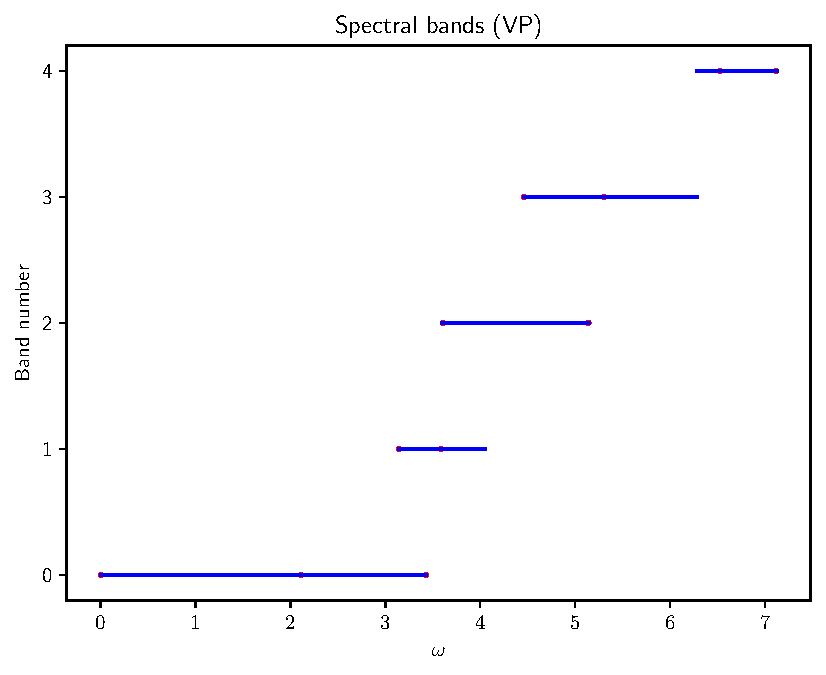
\includegraphics[scale=0.5]{CompositeCross-VP-SpectralBands.pdf}
	\caption[Eigenvalues of \eqref{eq:SI-WaveEqn}, computed via solution of problem \ref{prob:DiscVarProb}.]{\label{fig:CompositeCross-VP-SpectralBands} The eigenvalues belonging to the first 5 bands, approximated via the problem \ref{prob:DiscVarProb}.}
\end{figure}
We remark that there are no gaps between the spectral bands in this case, although gaps do open when $\alpha>0$ --- this will be demonstrated in section \ref{sec:SI-StrongDerivation}.
We can also notice that the eigenvalues within each band obey the symmetries in $\qm$ as expected from proposition \ref{prop:CrossInPlaneSymmetries}, by examining the dispersion relations in figure \ref{fig:VP_AllBands}.
\begin{figure}[t!]
	\centering
	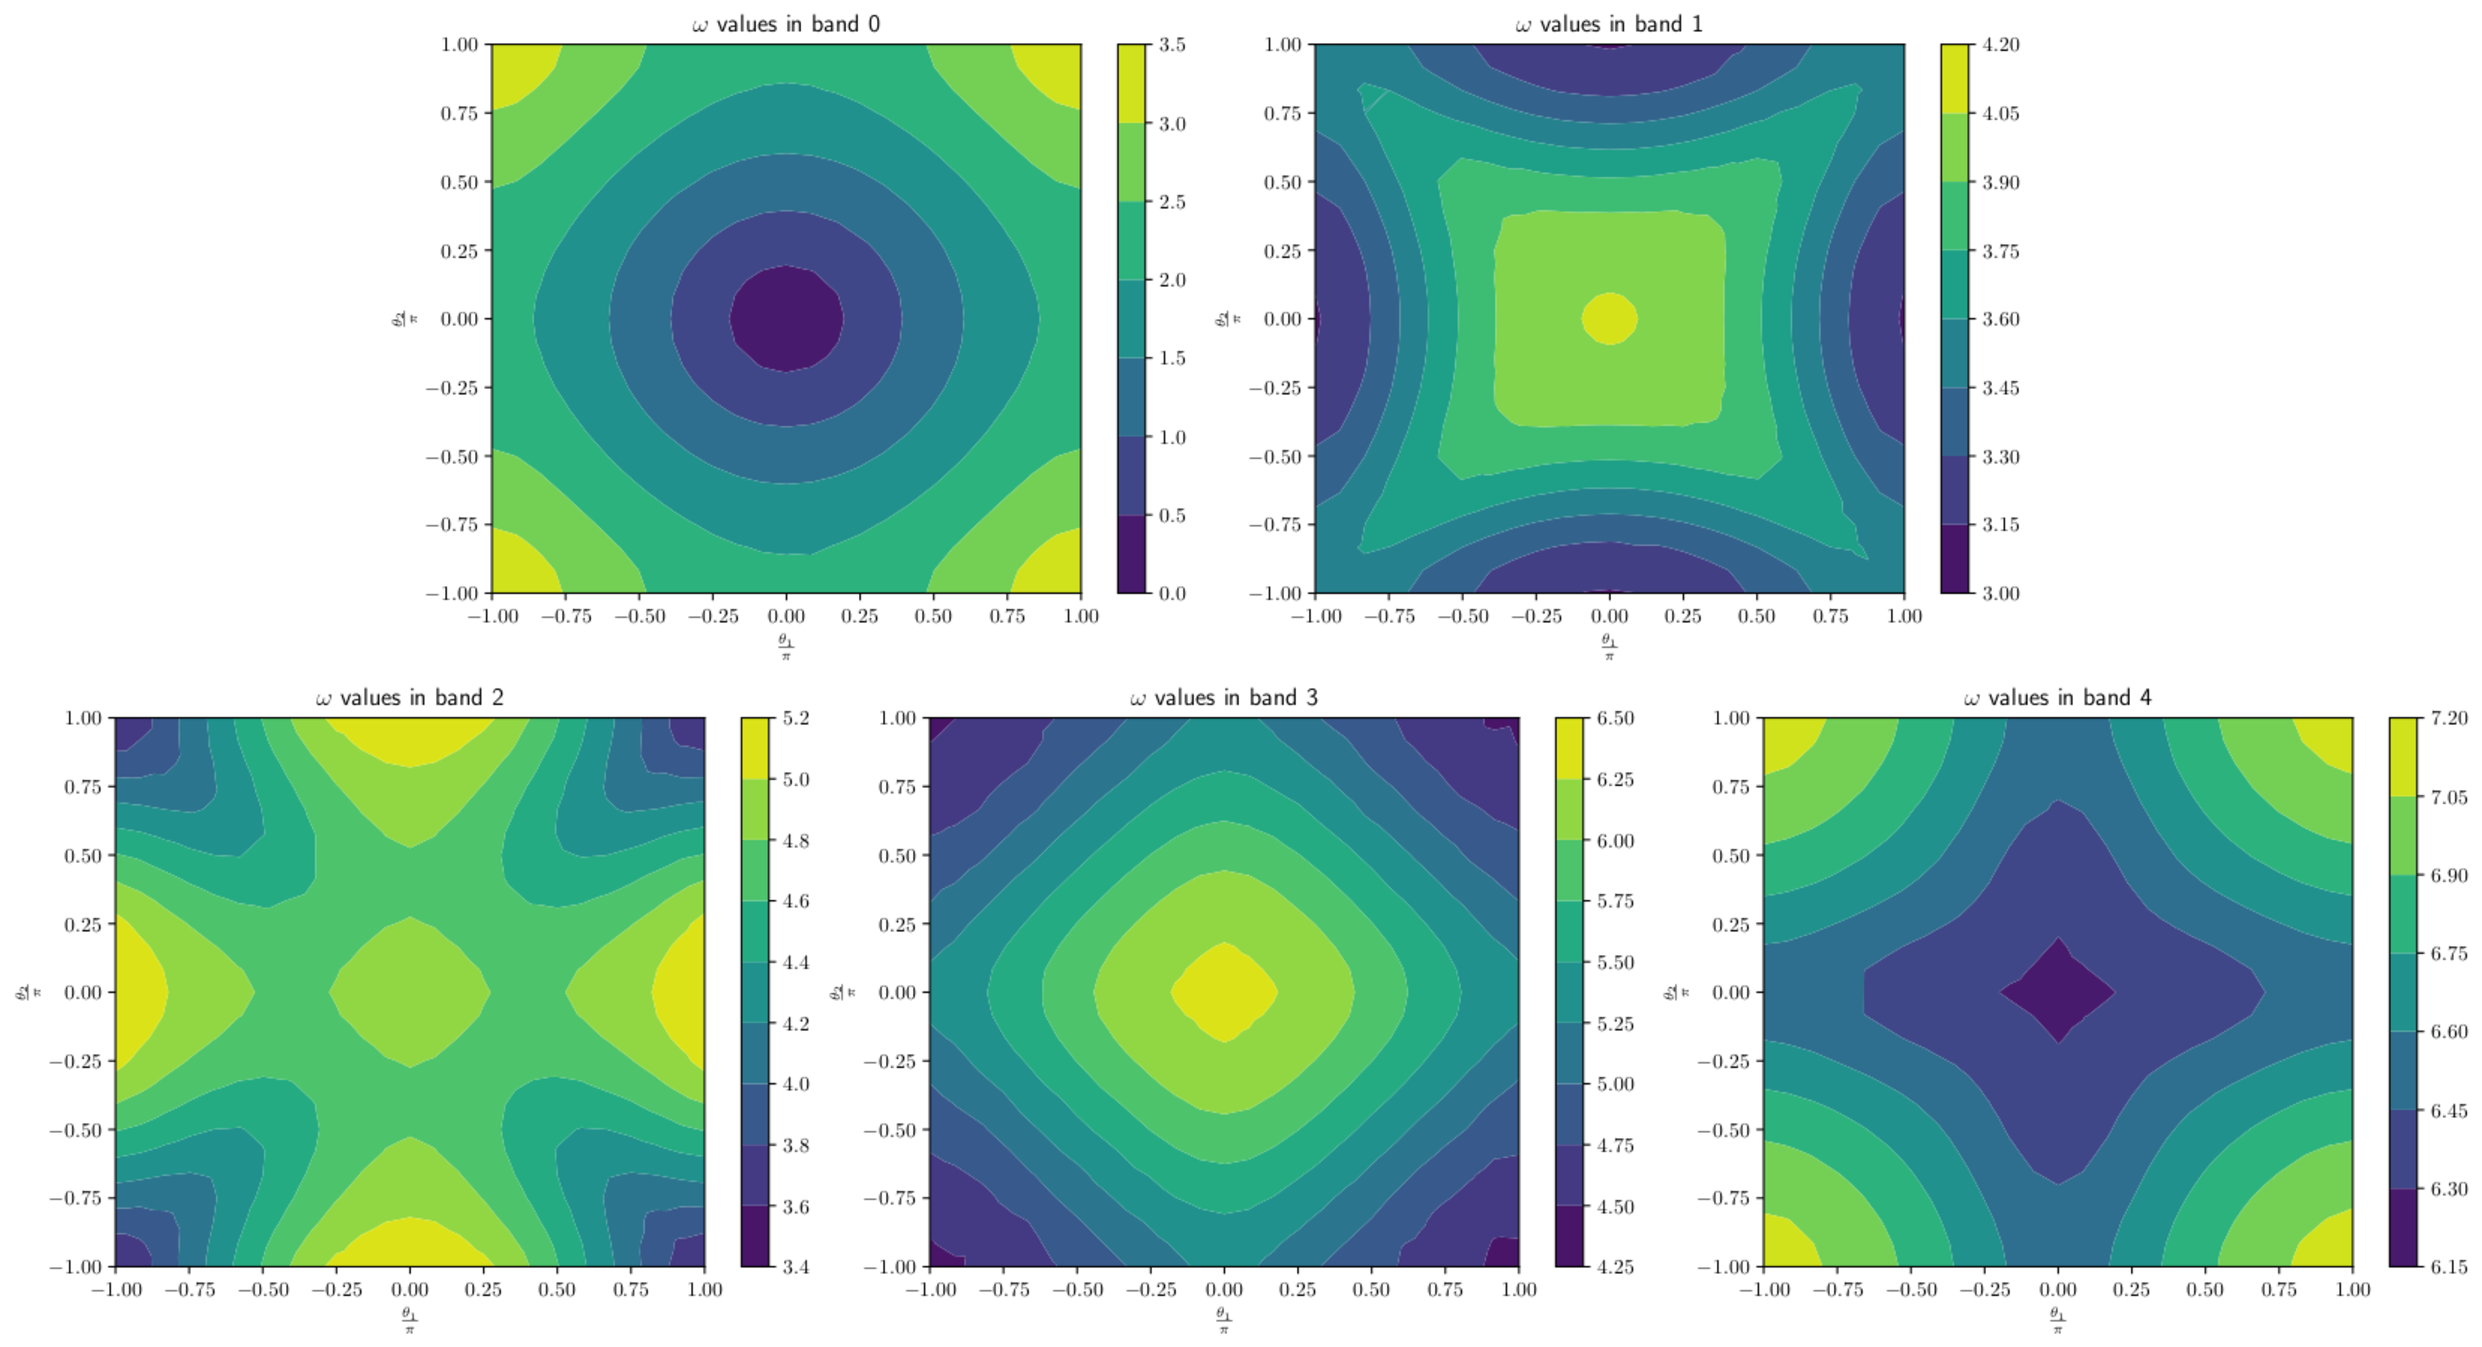
\includegraphics[width=\textwidth]{VP_2022-05-13-14-26_AllBands.pdf}
	\caption[Dispersion relations for the first 5 spectral bands of \eqref{eq:SI-WaveEqn}, computed via solution of problem \ref{prob:DiscVarProb}.]{\label{fig:VP_AllBands} The dispersion relations for the first 5 spectral bands, approximated via the problem \ref{prob:DiscVarProb}.}
\end{figure}

Although we have a method of computing the eigenvalues and eigenfunctions, we are no closer to understanding \emph{how} the presence of the skeleton and geometric contrast is affecting the problem \eqref{eq:SI-WaveEqn}.
It is also only by virtue of our analysis of the tangential gradients $\tgradSob{\ddom}{\ccompMes}$ that we are able to compute the integrals in \eqref{eq:SI-MinProblem}, and gain some insight into how we might want to approximate functions that live in $\tgradSob{\ddom}{\ccompMes}$.
In search of answers to these questions, we turn to the investigation in section \ref{sec:SI-StrongDerivation}.
We will also return to the idea of utilising a finite-element style approach to the solution of \eqref{eq:SI-WaveEqn} in our discussion in section \ref{sec:SI-Conc}.

% Derivation of the ``strong form" problem
\section{``Strong Formulation" of the Acoustic Approximation \eqref{eq:SI-WaveEqn}} \label{sec:SI-StrongDerivation}
Whilst we can choose to work directly from the min-max principle \eqref{eq:SI-VarProb} in an attempt to solve \eqref{eq:SI-WaveEqn}, we still do not have any explicit insights into how the presence of the skeleton is affecting the (solutions and eigenvalues of) this problem.
It is also desirable for us to move away from working with (approximations to) the tangential gradients themselves --- compared to classical gradients and derivatives, we do not have many tools to handle these objects numerically.
Therefore, in this section our goal is to derive a ``strong" formulation for \eqref{eq:SI-WaveEqn}, with motivations similar to those of sections \ref{sec:ScalarDerivation} and \ref{sec:3DSystemDerivation} --- we want to be able to analyse a more tractable problem, preferably in terms of objects familiar to us from classical calculus or chapter \ref{ch:ScalarSystem}.

Before we begin, we should consider what our intuition is telling us about the behaviour we expect from any solutions $u$ to \eqref{eq:SI-WeakWaveEqn}.
A good starting point is to consider how we expect our solutions to behave if we could (n\"{i}avely) interpret \eqref{eq:SI-WeakWaveEqn} in a strong sense.
Away from the skeleton, \eqref{eq:SI-WeakWaveEqn} looks like the usual acoustic approximation on a bounded domain, and so we expect our solution to possess sufficient regularity to be differentiated twice in the bulk and to look similar to the classical acoustic approximation here.
Regarding the skeleton, we know that solutions to the acoustic approximation on the singular structure corresponding to the skeleton possess two derivatives along the edges of $\graph$ (section \ref{sec:ScalarDerivation}), and are tied together through the vertex conditions.
So now we ask what should happen in the vicinity of the skeleton --- here we have (what we expect to be) a twice differentiable function in a bulk region $\ddom_i$ approaching its boundary, and so there should be ($L^2$) traces of $u$ and its normal derivative onto this boundary.
However this boundary coincides with (a subregion of) the skeleton, so the function $u$ should ``feel" the affect of these traces as it moves along the skeleton.
A partial converse is also expected; $u$ is twice differentiable along the skeleton, and given that $u$ \emph{also} has a trace onto the skeleton, we expect that these traces should be consistent with the function values from the bulk.
In summary, we should expect that \eqref{eq:SI-WeakWaveEqn} can be reformulated into a system that consists of the following components:
\begin{enumerate}[(a)]
	\item A (Helmholtz-like) PDE in each of the bulk regions, the solution to which has boundary traces matching the solution to a quantum graph problem on the inclusions.
	\item A 2nd-order quantum graph problem on the singular inclusions, with the edge ODEs involving or being influenced by the traces from the bulk regions.
	\item Conditions at the vertices of the graph to tie the quantum graph problem, and hence the PDE problems, together.
\end{enumerate}

Much like in sections \ref{sec:ScalarDerivation} and \ref{sec:3DSystemDerivation} we can work from \eqref{eq:SI-WeakWaveEqn} and the definition of $\tgradSob{\ddom}{\ccompMes}$ to obtain a system as described by (a)-(c).
The arguments we employ and the results we obtain are precisely those one would employ when applying the method of Lagrange multipliers to the problem \eqref{eq:SI-VarProb}.
Our starting point is the problem \eqref{eq:SI-WeakWaveEqn}, repeated here for ease of reading: find $\omega^2>0$ and non-zero $u\in\tgradSob{\ddom}{\ccompMes}$ such that
\begin{align*}
	\integral{\ddom}{ \tgrad_{\ccompMes}u\cdot\overline{\tgrad_{\ccompMes}\phi} }{\ccompMes}
	&= \omega^2 \integral{\ddom}{ u\overline{\phi} }{\ccompMes}, \quad\forall\phi\in\psmooth{\ddom}. \tag{\eqref{eq:SI-WeakWaveEqn} restated}
\end{align*}
We will need to make use of several standard integral identities, which we summarise below.
Let $D$ be an open Lipschitz domain, let $u\vert_{\partial D}$ denote the trace (of a suitably regular) function $u$ on $D$ into $\ltwo{\partial D}{S}$, and $n^D$ denote the exterior normal on the boundary of $D$.
\begin{itemize}
	\item For $u,v\in\gradSob{D}{\lambda_2}$ and $j\in\clbracs{1,2}$,
	\begin{align*}
		\integral{D}{ v\partial_j u + u\partial_j v }{\lambda_2}
		&= \integral{\partial D}{ u v n^D_j }{S}.
	\end{align*}
	\item For $u\in H^2\bracs{D,\lambda_2}, v\in\gradSob{D}{\lambda_2}$,
	\begin{align*}
		\integral{D}{ \grad u\cdot \grad v }{\lambda_2} 
		&=  - \integral{D}{ v\laplacian u }{\lambda_2} + \integral{\partial D}{ v\vert_{\partial D}\pdiff{u}{n^D}\vert_{\partial D} }{S}.
	\end{align*}
\end{itemize}
From the above, we can deduce that whenever $u\in H^2\bracs{D,\lambda_2}$ and $v\in\gradSob{D}{\lambda_2}$, we have that
\begin{align*}
	\integral{D}{ \tgrad u\cdot\overline{\tgrad v} }{\lambda_2}
	&= - \integral{D}{ \overline{v}\tgrad\cdot\tgrad u }{\lambda_2} + \integral{\partial D}{ \overline{v}\vert_{\partial D}\bracs{\tgrad u\cdot n^D}\vert_{\partial D} }{S}.
\end{align*}

We now begin the reformulation, starting by considering what happens when we test against functions supported in the bulk regions.
Suppose that the test function $\phi$ in \eqref{eq:SI-WeakWaveEqn} has support contained within the interior of one of the bulk regions $\ddom_i$, that is $\phi\in\csmooth{\ddom_i}$.
In this case \eqref{eq:SI-WeakWaveEqn} becomes
\begin{align*}
	\omega^2\integral{\ddom_i}{u\overline{\phi}}{\lambda_2} 
	&= \integral{\ddom_i}{ \grad u\cdot\overline{\grad\phi} - \rmi\qm\overline{\phi}\cdot\tgrad u + \rmi\qm  u\cdot\overline{\grad\phi} - \rmi^2\qm\cdot\qm u\overline{\phi} }{\lambda_2} \\
	&= \integral{\ddom_i}{ \grad u\cdot\overline{\grad\phi} - 2\rmi\qm\overline{\phi}\cdot\tgrad u - \rmi^2\qm\cdot\qm u\overline{\phi} }{\lambda_2}, \\
	\implies \integral{\ddom_i}{ \grad u\cdot\overline{\grad\phi} }{\lambda_2}
	&= \integral{\ddom_i}{ \bracs{\omega^2 u + 2\rmi\qm\cdot\tgrad u + \rmi^2\qm\cdot\qm u} \overline{\phi} }{\lambda_2}, 
\end{align*}
which holds for any $\phi\in\csmooth{\ddom_i}$.
Given that we also know that $u$ is $\ltwo{\partial\ddom_i}{S}$ (and is even $H^1$ in this space), this implies that $u\in \gradgradSob{\ddom_i}{\lambda_2}$ with
\begin{align*}
	\laplacian u &= -\bracs{ \omega^2 u + 2\rmi\qm\cdot\tgrad u + \rmi^2\qm\cdot\qm u }
\end{align*}
in $\ddom_i$, so we let $\laplacian^{\qm}:= \laplacian u + 2\rmi\qm\cdot\tgrad u + \rmi^2\qm\cdot\qm u$ and have that
\begin{subequations} \label{eq:SI-StrongForm} % This is so that the Strong System is coherently numbered, this spans most of the derivation so be careful!
\begin{align*}
	\laplacian_\qm u = -\omega^2 u, &\text{in } \ddom_i. \labelthis\label{eq:SI-BulkEqn}
\end{align*}
The additional regularity of the solution $u$ in the bulk regions provides equation \eqref{eq:SI-BulkEqn}, which matches our expectations in (a) of $u$ satisfying the acoustic approximation in the bulk regions, away from the skeleton.

Next we address what happens when we test against functions whose support straddles an edge $I_{jk}\in\edgeSet$.
For this we need to introduce a local labelling system for the bulk regions that are adjacent to $I_{jk}$.
Let $\ddom_{jk}^+$ be the bulk region whose boundary has non-empty intersection with $I_{jk}$ and whose exterior unit normal on $\partial\ddom_{jk}^+\cap I_{jk}$ is equal to $-n_{jk}$.
Similarly let $\ddom_{jk}^-$ be the bulk region whose boundary has non-empty intersection with $I_{jk}$ and whose exterior unit normal on $\partial\ddom_{jk}^-\cap I_{jk}$ is equal to $n_{jk}$.
Note the sign convention; this is chosen because the region $\ddom_{jk}^+$ is ``to the right" of $I_{jk}$ as viewed from the local coordinate system $y_{jk}=\bracs{n_{jk}, e_{jk}}$, and $\ddom_{jk}^-$ is ``on the left" --- see figure \ref{fig:Diagram_SI-AdjacentBulkRegions}.
\begin{figure}[t!]
	\centering
	\includegraphics[scale=1.0]{Diagram_SI-AdjacentBulkRegions.pdf}
	\caption[Labelling convention for bulk regions adjacent to a skeleton edge.]{\label{fig:Diagram_SI-AdjacentBulkRegions} Labelling convention for regions adjacent to an edge $I_{jk}$.}
\end{figure}
Now consider \eqref{eq:SI-WeakWaveEqn} when $\phi$ is taken to have compact support that intersects (the interior of) an edge $I_{jk}$, the adjacent bulk regions $\ddom_{jk}^+$ and $\ddom_{jk}^-$, and no other parts of $\graph$.
Equation \eqref{eq:SI-WeakWaveEqn} then implies that
\begin{align*}
	\integral{\ddom}{ \omega^2 u\overline{\phi} - \tgrad_{\lambda_{jk}}u\cdot\overline{\tgrad_{\lambda_{jk}}\phi} }{\lambda_{jk}}
	&= \integral{\ddom}{ \tgrad u\cdot\overline{\tgrad\phi} - \omega^2 u\overline{\phi} }{\lambda_2} \\
	&= \integral{\ddom_{jk}^+}{ \tgrad u\cdot\overline{\tgrad\phi} - \omega^2 u\overline{\phi} }{\lambda_2}
	+ \integral{\ddom_{jk}^-}{ \tgrad u\cdot\overline{\tgrad\phi} - \omega^2 u\overline{\phi} }{\lambda_2}.
\end{align*}
We know that $u\in \gradgradSob{\ddom_{jk}^{\pm}}{\lambda_2}$ for both $\ddom_{jk}^+$ and $\ddom_{jk}^-$, and so $u$ and its normal derivative possess have $L^2$-traces onto $I_{jk}$.
Using the notation $\tgrad u\cdot n_{jk} = \pdiff{u}{n_{jk}} + \rmi\qm u\cdot n_{jk}$; and denoting the trace of $u\in\gradgradSob{\ddom_{jk}^{\pm}}{\lambda_2}$ onto the boundary $\partial\ddom^{\pm}$ by $u^{\pm}$, we have that
\begin{align*}
	\integral{\ddom}{ & \omega^2 u\overline{\phi} - \tgrad_{\lambda_{jk}}u \cdot\overline{\tgrad_{\lambda_{jk}}\phi} }{\lambda_{jk}} \\
	&= \integral{\ddom_{jk}^+}{ -\overline{\phi}\bracs{ \laplacian_{\qm} u + \omega^2 u } }{\lambda_2}
	+ \integral{\ddom_{jk}^-}{ -\overline{\phi}\bracs{ \laplacian_{\qm} u + \omega^2 u } }{\lambda_2}
	+ \integral{\partial\ddom_{jk}^+}{ -\overline{\phi}\bracs{\tgrad u\cdot n_{jk}}^{+} }{S} \\
	&\qquad + \integral{\partial\ddom_{jk}^-}{ \overline{\phi}\bracs{\tgrad u\cdot n_{jk}}^{-} }{S},
\end{align*}
since the exterior normal to $\ddom_{jk}^{\pm}$ is $\mp n_{jk}$.
Given \eqref{eq:SI-BulkEqn} and the support of $\phi$, this further implies that
\begin{align*}
	\integral{\ddom}{ \omega^2 u\overline{\phi} - \tgrad_{\lambda_{jk}}u\cdot\overline{\tgrad_{\lambda_{jk}}\phi} }{\lambda_{jk}}
	&= \integral{I_{jk}}{ \overline{\phi}\sqbracs{\bracs{\tgrad u\cdot n_{jk}}^- - \bracs{\tgrad u\cdot n_{jk}}^+} }{S} \\
	&= \int_0^{l_{jk}} \overline{\phi}\sqbracs{\bracs{\tgrad u\cdot n_{jk}}^- - \bracs{\tgrad u\cdot n_{jk}}^+} \ \md y,
\end{align*}
where we have used $r_{jk}$ to parametrise\footnote{In the interest of brevity, we have suppressed composition with $r_{jk}$ --- we rely on the domain of integration to imply composition of the integrand with $r_{jk}$.} the boundary $I_{jk}$.
Changing variables via $r_{jk}$ in the integral on the left hand side too, substituting the known form for the tangential gradients, and rearranging then provides us with
\begin{align*}
	\int_0^{l_{jk}} \bracs{u^{(jk)}}'\overline{\phi}' \ \md y
	&= \int_0^{l_{jk}} \overline{\phi}\sqbracs{ \bracs{\tgrad u\cdot n_{jk}}^- - \bracs{\tgrad u\cdot n_{jk}}^+ \right. \\
	&\qquad \left. - \omega^2 u^{(jk)} - 2\rmi\qm_{jk}\bracs{u^{(jk)}}' - \bracs{\rmi\qm_{jk}}^2 u^{(jk)} } \ \md y,
\end{align*}
which holds for all smooth $\phi$ with support contained in the interior of $I_{jk}$.
Since the factor in square brackets is $\ltwo{\sqbracs{0,l_{jk}}}{y}$, we can deduce that $u^{(jk)}\in\gradgradSob{\sqbracs{0,l_{jk}}}{y}$, and
\begin{align*}
	- \bracs{\diff{}{y} + \rmi\qm_{jk}}^2u^{(jk)} 
	&= \omega^2 u^{(jk)} + \bracs{\tgrad u\cdot n_{jk}}^+ - \bracs{\tgrad u\cdot n_{jk}}^-,
	&\qquad\text{in } \sqbracs{0,l_{jk}}.
\end{align*}
If we additionally recall that the trace of $u$ from the bulk regions $\ddom_{jk}^{\pm}$ is equal to $u^{(jk)}$, we can eliminate part of the trace-terms to obtain
\begin{align} \label{eq:SI-InclusionEqn}
	- \bracs{\diff{}{y} + \rmi\qm_{jk}}^2 u^{(jk)} 
	&= \omega^2 u^{(jk)} + \bracs{\grad u\cdot n_{jk}}^+ - \bracs{\grad u\cdot n_{jk}}^-,
	&\qquad\text{in } I_{jk}.
\end{align}
This provides us with part (b) from our intuitive argument --- on the edges of the graph we have the second-order differential equation from chapter \ref{ch:ScalarSystem}, but with the addition of a term capturing the differences in the trace of the normal derivative of $u$ from either side of the inclusion.
It is worth remarking that if our inclusions were merely interfaces, we would simply obtain an algebraic equation in the difference of the normal derivative traces on the $I_{jk}$.
Giving the edges a notion of length, even if it is only one-dimensional length within a two-dimensional domain, has resulted in the difference (or ``jump") in the normal derivatives directly influencing the behaviour of $u$ on the inclusions.
Conversely, the requirement that the traces of $u$ from $\ddom_{jk}^{\pm}$ be equal to $u^{(jk)}$ also means that the behaviour of $u$ on the inclusions will affect the solution in the bulk regions.
This coupling is similar to a ``feedback loop"; the solution in the bulk exerts influence on the edges through the traces of the normal derivatives, and the solution on the inclusions exerts influence on the bulk via the requirement that the traces coincide with the values on the inclusion.

The final question we need to ask concerns the solution $u$ in the vicinity of a vertex, or more precisely when $\phi$ has support containing a vertex $v_j$ (and without loss of generality, no other vertices).
The process is straightforward; we aim to proceed as before and use \eqref{eq:SI-BulkEqn} and \eqref{eq:SI-InclusionEqn} to cancel terms on the inclusions and in the bulk regions, leaving us with a ``vertex condition", however we require one final set of temporary notation to transcribe the argument.
Fix $v_j\in\vertSet$ for each $I_{jk}\in J(v_j)$ let $\beta_{jk}$ be the anticlockwise angle between the segment $I_{jk}$ and the $v_j+\hat{x}_1$ direction.
The $\clbracs{\beta_{jk}}$ can then be ordered by size, and correspondingly we can also order the $I_{jk}\in J(v_j)$, writing
\begin{align*}
	\beta_{jk_1} < \beta_{jk_2} < ... < \beta_{jk_{\deg(v_j)}}, 
	\qquad I_{jk_1} < I_{jk_2} < ... < I_{jk_{\deg(v_j)}}.
\end{align*}
Also adopt a cyclic convention, where $k_0 = k_{\deg(v_j)}$ and $k_{\deg(v_j)+1} = k_1$.
Now, for each $l\in\clbracs{1,...,\deg(v_j)}$ let $\ddom_{jk_l}$ be the bulk region that lies between (in the sense of the angles $\beta_{jk_{l-1}}$ and $\beta_{jk_l}$) $I_{jk_{l-1}}$ and $I_{jk_l}$.
This labelling can be visualised in figure \ref{fig:Diagram_SI-JunctionLabelling}.
\begin{figure}[t!]
	\centering
	\includegraphics[scale=1.5]{Diagram_SI-JunctionLabelling.pdf}
	\caption[Labelling convention for bulk regions surrounding a vertex.]{\label{fig:Diagram_SI-JunctionLabelling} The labelling conventions for the bulk regions and edges surrounding a vertex.}
\end{figure}

Fix $v_j\in\vertSet$ and let $\phi\in\psmooth{\ddom}$ have support that contains $v_j$ and no other points in $\vertSet$.
With such a $\phi$, the following equalities hold;
\begin{align*}
	\integral{\ddom}{ \tgrad u\cdot\overline{\tgrad\phi} - \omega^2u\overline{\phi} }{\lambda_2}
	&= \sum_{l} \integral{\ddom_l}{ \tgrad u\cdot\overline{\tgrad\phi} - \omega^2u\overline{\phi} }{\lambda_2} \\
	&= \sum_{l} \integral{\ddom_l}{ -\overline{\phi}\bracs{ \laplacian_{\qm} u + \omega^2 u } }{\lambda_2}
	+ \integral{\partial\ddom_l}{ \overline{\phi}\tgrad u\cdot n_{jk_l} }{S} \\
	&= \sum_l \integral{I_{jk_l}}{ \overline{\phi}\tgrad u\cdot n_{jk_l} }{S} + \integral{I_{jk_{l-1}}}{ \phi\tgrad u\cdot n_{jk_{l-1}} }{S} \\
	&= \sum_l \integral{I_{jk_l}}{ \overline{\phi}\bracs{ \bracs{\tgrad u\cdot n_{jk_l}}^- - \bracs{\tgrad u\cdot n_{jk_l}}^+ } }{S}, \\
	\integral{\ddom}{ \tgrad_{\ccompMes} u\cdot\overline{\tgrad_{\ccompMes}\phi} - \omega^2u\overline{\phi} }{\ddmes}
	&= \sum_l \integral{I_{jk_l}}{ -\overline{\phi}\bracs{\bracs{\diff{}{y}+\rmi\qm_{jk_l}}^2 u^{(jk_l)} + \omega^2 u^{(jk_l)}} }{\lambda_{jk_l}} \\
	&\qquad + \sum_l \sqbracs{ \bracs{\pdiff{}{n}+\rmi\qm_{jk_l}} u^{(jk_l)}(v_j)\overline{\phi}(v_j) }.
\end{align*}
Thus, equation \eqref{eq:SI-WeakWaveEqn} becomes
\begin{align*}
	\alpha_j\omega^2 u(v_j)\overline{\phi}(v_j)
	&= \sum_l \clbracs{ \integral{I_{jk_l}}{ \overline{\phi}\bracs{ \bracs{\tgrad u\cdot n_{jk_l}}^- - \bracs{\tgrad u\cdot n_{jk_l}}^+ } }{S} \right. \\
	&\qquad \left.	+ \integral{I_{jk_l}}{ -\overline{\phi}\bracs{\bracs{\diff{}{y}+\rmi\qm_{jk_l}}^2 u^{(jk_l)} + \omega^2 u^{(jk_l)}} }{\lambda_{jk_l}} \right. \\
	&\qquad \left.	+ \sqbracs{ \bracs{\pdiff{}{n}+\rmi\qm_{jk_l}} u^{(jk_l)}(v_j)\overline{\phi}(v_j) } } \\
	&= \sum_l \sqbracs{ \bracs{\pdiff{}{n}+\rmi\qm_{jk_l}} u^{(jk_l)}(v_j)\overline{\phi}(v_j) }
	&\quad\text{using \eqref{eq:SI-InclusionEqn}}, \\
	\implies \alpha_j\omega^2 u(v_j)\overline{\phi}(v_j)
	&= \sum_l \bracs{\pdiff{}{n}+\rmi\qm_{jk_l}} u^{(jk_l)}(v_j), \labelthis\label{eq:SI-VertexCondition}
\end{align*}
\end{subequations} % last equation that we needed in the strong form has been provided, close off the subequations environment
since $\phi(v_j)$ is arbitrary.
In addition to continuity of $u$ at each of the vertices, we have found that $u$ also adheres to the same Wentzell condition at each of the vertices as in the case of a singular structure.

The system \eqref{eq:SI-StrongForm}\footnote{We call \eqref{eq:SI-StrongForm} ``strong" since it is no longer understood in a variational sense, and its relation to \eqref{eq:SI-WaveEqn} is akin to the relationship between the strong and weak forms of PDEs.}, 
\begin{subequations}
	\begin{align*}
		-\laplacian_\qm u 
		&= \omega^2 u 
		&\text{in } \ddom_i, \tag{\eqref{eq:SI-BulkEqn} restated} \\
		- \bracs{\diff{}{y} + \rmi\qm_{jk}}^2u^{(jk)}  
		&= \omega^2 u^{(jk)} + \bracs{\bracs{\grad u\cdot n_{jk}}^+ - \bracs{\grad u\cdot n_{jk}}^-}
		&\text{in } I_{jk}, \tag{\eqref{eq:SI-InclusionEqn} restated} \\
		\sum_{j\con k} \bracs{\pdiff{}{n}+\rmi\qm_{jk}} u^{(jk)}(v_j) 
		&= \alpha_j\omega^2 u(v_j)
		&\text{at } v_j\in\vertSet, \tag{\eqref{eq:SI-VertexCondition} restated}
	\end{align*}
\end{subequations}
The system is composed of two differential equations (the PDE \eqref{eq:SI-BulkEqn} on the bulk, and the ODE \eqref{eq:SI-InclusionEqn} on the skeleton) coupled through the vertex condition \eqref{eq:SI-VertexCondition} and the requirement that the traces from adjacent regions match the function values on the skeleton --- matching our expectations from before.
The objects involved are more familiar, being a combination of classical gradients and the essentially one-dimensional tangential derivatives studied in section \ref{sec:3DGradSobSpaces}.
We also expect the system \eqref{eq:SI-StrongForm} to be easier to work with numerically (compared to \eqref{eq:SI-VarProb}), due to the interaction between the bulk regions and skeleton being made explicit.
There are however two ``scales" on which a solution $u$ behaves, being 2D in the bulk and 1D on the skeleton, and we need resolution in both of them.

It is worth making some remarks here to reconnect \eqref{eq:SI-StrongForm} with the physical (or ``dimensionfull") material it represents.
The domain on which the system \eqref{eq:SI-StrongForm} is posed is motivated by the ``visual" limit of the acoustic approximation on a composite material with thin inclusions that are shrinking to zero thickness.
The \emph{material} properties in the background material and on the inclusions\footnote{That is, the permittivities and under the non-magnetic assumption, permeabilities.} in these domains are identical, but there is (geometric) contrast between the edge and vertex volumes of the inclusions.
Indeed, the (dimensionless) parameters $\alpha_j$ only appear in one of the three equations \eqref{eq:SI-VertexCondition}, because this is the only equation in which the vertex and edge regions interact.
%This is directly analogous to the situation one ends in when studying composite materials with contrasting material properties; the dimensionless parameters representing the contrast appear in (what is normally a boundary condition) relating the values of the solution across the interface between the inclusion and background material.
It is natural to ask whether our approach allows for the presence of material contrast, as well as geometric contrast, and how this might affect our problem formulation and the system \eqref{eq:SI-StrongForm}.
With this in mind, let us introduce some material contrast between the bulk regions and the skeleton, represented through the (dimensionless) function
\begin{align*}
	\epsilon_m =
	\begin{cases} 1 & x\in\ddom_i, \\ \epsilon & x\in\graph, \end{cases}
\end{align*}
where $\epsilon$ is the parameter quantifying the contrast between the material properties (the permittivities in this context) on the skeleton and in the bulk.
We also let $m>0$ (whose interpretation will become clear shortly) and modify the system \eqref{eq:SI-WaveEqn} slightly to account for this contrast, considering the problem
\begin{align*}
	-\epsilon_m^{-1}\laplacian_{\ccompMes}^{\qm} u &= \omega^2 u,
	\qquad u\in\tgradSob{\ddom}{\lambda_2^{m\dddmes}},
\end{align*}
understood as the problem of finding $u\in\tgradSob{\ddom}{\lambda_2^{m\dddmes}}$ and $\omega^2>0$ such that
\begin{align} \label{eq:SI-ContrastWeakWaveEqn}
	\integral{\ddom}{ \epsilon_m^{-1}\tgrad_{\ccompMes}u\cdot\overline{\tgrad_{\ccompMes}\phi} }{\lambda_2^{m\dddmes}}
	&= \omega^2 \integral{\ddom}{ u\overline{\phi} }{\lambda_2^{m\dddmes}}, \quad\forall\phi\in\psmooth{\ddom}.
\end{align}
Utilising an identical argument to the above, \eqref{eq:SI-ContrastWeakWaveEqn} admits the ``strong" formulation
\begin{subequations}
	\begin{align*}
		-\laplacian_\qm u 
		&= \omega^2 u 
		&\text{in } \ddom_i, \\
		- \epsilon^{-1}\bracs{\diff{}{y} + \rmi\qm_{jk}}^2u^{(jk)}  
		&= \omega^2 u^{(jk)} + \recip{m}\bracs{\bracs{\grad u\cdot n_{jk}}^+ - \bracs{\grad u\cdot n_{jk}}^-}
		&\text{in } I_{jk}, \\
		m\epsilon^{-1}\sum_{j\con k} \bracs{\pdiff{}{n}+\rmi\qm_{jk}} u^{(jk)}(v_j) 
		&= m\omega^2 \alpha_j u(v_j)
		&\text{at } v_j\in\vertSet.
	\end{align*}
\end{subequations}
Let us consider the case where $\alpha_j=0$ and examine the high-index limit $\epsilon\rightarrow0$ --- we obtain the system
\begin{subequations}
	\begin{align*}
		\laplacian_\qm u 
		&= \omega^2 u 
		&\text{in } \ddom_i, \\
		\omega^2 u^{(jk)}
		&= \bracs{\bracs{\grad u\cdot n_{jk}}^- - \bracs{\grad u\cdot n_{jk}}^+}
		&\text{in } I_{jk},
	\end{align*}
\end{subequations}
which is a realisation of the system \eqref{eq:Intro-KuchFigQGLimit} upon identifying $W=m^{-1}$ and rescaling the spectral parameter $\omega^2=zm^{-1}$ by the constant $m$.
In the study \cite{figotin1998spectral}, the spectrum of \eqref{eq:Intro-KuchFigQGLimit} was shown to coincide with the limit of the spectra of the acoustic equation on the domains illustrated in figure  \ref{fig:Diagram_KF-DoubleLimitStudy} in the limit that the inclusion thickness $\delta\rightarrow0$ simultaneously with $\epsilon\bracs{\delta}\delta\rightarrow m$.
By including the ``mass" $m = \lim_{\delta\rightarrow0}\delta\epsilon\bracs{\delta}$ as a prefactor to the singular measure $\dddmes$ that supports the corresponding singular limit of this region (the skeleton), our variational problem also describes the effective problem.
We also remark that the parameter $m$ fulfils a similar role to the $\alpha_j$; in being the parameter that describes the limiting behaviour of the interactions between the shrinking thickness $\delta$ and increasing permittivity $\epsilon$, and it is introduced in precisely the same manner as $\alpha_j$ --- as a prefactor to the relevant measure.
In light of this, our problem \eqref{eq:SI-WaveEqn} also suggests the effective problem one might obtain if the study \eqref{eq:Intro-KuchFigQGLimit} was extended to \emph{also} encompass possible geometric contrast between the edge and vertex regions of the shrinking inclusions (that is, reintroducing non-zero $\alpha_j$).

Our final comments on the system \eqref{eq:SI-StrongForm} pertain to the form of the ODEs on the skeleton \eqref{eq:SI-InclusionEqn} --- in particular the presence of a coupling between the flux across the skeleton and the ``diffusion" (the second-derivative operator) along the skeleton.
Analogous conditions (and equations in the bulk) are derived in the study \cite{cherednichenko2019homogenisation} in a similar domain setup, but concerning the problem of homogenisation for the equations of (linearised) elasticity.
The effective problem obtained in this study also exhibited coupling between the diffusion along the (equivalent of the) skeleton and flux across the skeleton\footnote{It is noted in \cite{cherednichenko2019homogenisation} that such conditions, in which coupling diffusion along a boundary to diffusion along said boundary, belong to the (very broad) class of \emph{Ventcel}' conditions \cite{venttsel1959boundary}. This is the same class that the \emph{Wentzell} conditions for quantum graphs belong to --- it is likely that Wentzell and Ventcel' are different spellings of the same translated name.}.
Again we highlight that the material considered in \cite{cherednichenko2019homogenisation} did not consider different geometric contrasts (between the vertex and edge regions), so there is no analogous equation to \eqref{eq:SI-VertexCondition} appears in the effective problem, much like in the system obtained from \eqref{eq:Intro-KuchFigQGLimit}.

Having obtained \eqref{eq:SI-StrongForm} from \eqref{eq:SI-WaveEqn} lends further weight to our motivations for using \eqref{eq:SI-WaveEqn} (and the other variational problems we have studied) as a predictive tool, as well as reinforcing the idea that \eqref{eq:SI-WaveEqn} does provide a model of ``wave propagation" on structures with singular components.
Indeed, our construction and setup of the problem \eqref{eq:SI-WaveEqn} enables us to provide the definition of a (candidate) limit operator for the acoustic equation on a material with thin inclusions, that possesses both geometric and material contrasts some geometric contrast.
The reduction under certain regimes to the problem \eqref{eq:Intro-KuchFigQGLimit}; and the similarities with the effective problem derived in \cite{cherednichenko2019homogenisation}, further support the idea that our variational problems can be used to provide the definitions of the limiting operators in such contexts.
Our attempts to compute the spectra of such problems gain additional traction because of this --- being able to do so enables exploration of the parameter space spanned by the ``contrast parameters" ($\alpha_j$, $m$, and potentially others) and thus insights into the behaviours of physical materials under the corresponding asymptotic limits.

% Ideas for numerical solution of the strong problem
\subsection{Solution of \eqref{eq:SI-StrongForm} via Finite-Differences} \label{ssec:SI-FDMMethod}
Now that we have the problem \eqref{eq:SI-StrongForm} to work with, we can attempt to solve \eqref{eq:SI-WaveEqn} through a formulation that involves familiar gradients and derivatives, rather than the more abstract tangential gradients.
Before we do so, it is convenient to notice that we can move the ``trace" terms in \eqref{eq:SI-InclusionEqn} to the left-hand-side to obtain the slightly nicer (in terms of the numerics that follow) looking system
\begin{subequations} \label{eq:SI-FDMEquationsToDisc}
	\begin{align}
		-\laplacian_\qm u 
		&= \omega^2 u 
		&\text{in } \ddom_i, \label{eq:SI-FDMBulk} \\
		- \bracs{\diff{}{y} + \rmi\qm_{jk}}^2u^{(jk)}  - \bracs{\bracs{\grad u\cdot n_{jk}}^+ - \bracs{\grad u\cdot n_{jk}}^-}
		&= \omega^2 u^{(jk)},
		&\text{in } I_{jk}, \label{eq:SI-FDMSkeleton} \\
		\sum_l \bracs{\pdiff{}{n}+\rmi\qm_{jk_l}} u^{(jk_l)}(v_j) 
		&= \alpha_j\omega^2 u(v_j)
		&\text{at } v_j\in\vertSet. \label{eq:SI-FDMVertex}
	\end{align}
\end{subequations}
We have now placed everything except terms involving the spectral parameter on the left hand side of \eqref{eq:SI-FDMEquationsToDisc}, and our goal now is to devise a numerical scheme to approximate the action of the ``operators" on the left-hand-side, and from that approximate the spectrum of the problem.

Our idea is as follows; we recognise that $u$ is twice differentiable (in the familiar, classical sense) in each of the bulk regions and along each of the skeleton edges, so we can look to to approximate the spectrum of our problem by approximating $u$ through a (somewhat n{\"i}ave) finite-difference approximation in each of the bulk regions and skeleton edges, and tying these ``region-wise" approximations together.
To this end, we take each of the bulk regions $\ddom_i$, and place nodes $\tau_j\in\overline{\ddom}_{i}$ appropriately, so as to write finite difference approximations for $\laplacian_{\qm}u$ at each node $\tau_j\in\ddom_i$.
Note that, since $u$ is not required to be differentiable (in the classical sense) across the skeleton, it is important that any finite difference approximation at $\tau_j$ only uses the values of $u$ at other nodes in $\overline{\ddom}_{i}$.
In placing nodes in $\overline{\ddom}_{i}$, we will also end up with nodes placed on the portion of the skeleton (and vertices) that form part of $\partial\ddom_i$.
Since $u$ is twice differentiable along the skeleton, the placement of these nodes allows us to derive finite-difference approximations for the derivatives in \eqref{eq:SI-FDMSkeleton}.
The traces of the normal derivates (in \eqref{eq:SI-FDMSkeleton}) can also be approximated via one-sided differences using suitable nodes from each of the adjacent bulk regions.
Finally, an approximation for \eqref{eq:SI-FDMVertex} can be derived for nodes that lie at vertices $v_j\in\vertSet$, using the nodes that lie on edges that connect to $v_j$.
We will come to discuss some of the difficulties with the general application of this procedure after our illustrative example.
For now, let us assume we have approximations for the action of the gradient and derivative, so that the action of the left-hand-side of \eqref{eq:SI-FDMEquationsToDisc} is approximated through the action of a matrix $\mathcal{F}$ on the vector $U = \bracs{u_j}^\top$, where $u_j:=u\bracs{\tau_j}$.
We then approximate the system \eqref{eq:SI-FDMEquationsToDisc} by the matrix-eigenvalue problem involving $\mathcal{F}$.

Let us begin by illustrating this approach using the cross in the plane geometry.
We first discretise $\ddom$ into a uniform mesh consisting of $N\times N$ nodes $\tau_{p,q} = \bracs{(p-1)h,(q-1)h}$ for $p,q\in\clbracs{1,...,N}$, with a mesh width of $h = \recip{N-1}$, and write $u_{p,q} = u\bracs{\tau_{p,q}}$.
It is important to note at this early stage that we can utilise a uniform mesh thanks to the rather simple geometry of the skeleton, and in general the meshing process will be more complex (see the discussion at the end of this section).
Note that there is no need to place nodes along both of the periodic edges of $\ddom$, so long as we keep track of which nodes are connected by periodicity, but for notational purposes it is convenient to include such nodes in our description.
Proceeding with the discretisation of the above equations, $u$ is twice differentiable in the bulk region $\ddom^{\circ}$, and so at points $\tau_{p,q}\not\in\graph$ we can discretise as
\begin{align*}
	-\laplacian_\qm u\bracs{\tau_{p,q}} &\approx 
	\bracs{\abs{\qm}^2 + 4h^{-2}}u_{p,q}
	-h^{-1}\bracs{h^{-1} + \rmi\qm_1}u_{p+1,q}
	-h^{-1}\bracs{h^{-1} - \rmi\qm_1}u_{p-1,q} \\
	&\qquad -h^{-1}\bracs{h^{-1} + \rmi\qm_2}u_{p,q+1}
	-h^{-1}\bracs{h^{-1} - \rmi\qm_2}u_{p,q-1}, \labelthis\label{eq:SI-FDMBulkDiscretise}
\end{align*}
using centred differences.
One can also use forward (also known as left) or backward (a.k.a right) differences to approximate the $\laplacian_{\qm}$ operator --- this will likely be necessary for more complex skeleton geometries as was hinted at previously.
Also worth noting is that, should one choose not to use (or be unable to use) a uniform mesh, one will still obtain a similar expression to \eqref{eq:SI-FDMBulkDiscretise} for the approximation of $\laplacian_\qm u$ at a node $\tau\not\in\graph$, but in terms of the values of $u$ at, and the distances to, the ``nearest neighbour" nodes to $\tau$.

For nodes $\tau_{p,q}\in I_{jk}$ (for either $I_{jk}=I_h$ or $I_v$), our finite difference approximations become slightly more complex as we are forced to consider the nearest nodes to $\tau_{p,q}$ that lie in the directions $e_{jk}$ and $n_{jk}$.
This is because $u$ is only twice differentiable \emph{along the skeleton}, so we must approximate $\bracs{\diff{}{y} + \rmi\qm_{jk}}^2u^{(jk)}$ through nodal values ``adjacent" to $\tau_{p,q}$ in the $e_{jk}$ and $-e_{jk}$ directions.
For the normal-derivative trace terms, we use one-sided finite differences to approximate these values at $\tau_{p,q}$, which involves the values of $u$ at the nodes ``adjacent" to $\tau_{p,q}$ in the $n_{jk}$ and $-n_{jk}$ directions.
For general skeleton geometries these requirements will contribute to the complications with meshing the domain, but since the edges are aligned with the coordinate axes in the cross-in-the-plane geometry, the vectors $e_{jk}$ and $n_{jk}$ are also aligned with the coordinate axes and the discretisation proceeds easily.
Those $\tau_{p,q}$ that lie on the horizontal edge $I_h$ have $q=0$ and $p\neq0$, so our finite difference approximation is
\begin{align*}
	- & \bracs{\diff{}{y} + \rmi\qm_{jk}}^2 u_{p,0} - \bracs{\bracs{\grad u_{p,0}\cdot n_{jk}}^+ - \bracs{\grad u_{p,0}\cdot n_{jk}}^-} \\
	& \quad\approx \bracs{\qm_1^2 + 2h^{-1} + 2h^{-2}}u_{p,0}
	- h^{-1}\bracs{h^{-1} + \rmi\qm_1}u_{p+1,0}
	- h^{-1}\bracs{h^{-1} - \rmi\qm_1}u_{p-1,0} \\
	& \quad - h^{-1}u_{p,1} - h^{-1}u_{p,-1}. \labelthis\label{eq:SI-FDMHorzEdgeDiscretise}
\end{align*}
Here we have used centred differences along the edge $I_h$, identifying that the nodes $\tau_{p-1,0}, \tau_{p+1,0}$ are the adjacent nodes in the $x_1 (= e_h)$ direction.
The traces cause the introduction of the terms $u_{p,-1}$ and $u_{p,1}$, since $-x_2 = n_h$.
Analogously, nodes $\tau_{p,q}$ on the vertical edge $I_v$ have $p=0$ and $q\neq0$, and the finite difference approximation is
\begin{align*}
	- & \bracs{\diff{}{y} + \rmi\qm_{jk}}^2 u_{0,q} - \bracs{\bracs{\grad u_{0,q}\cdot n_{jk}}^+ - \bracs{\grad u_{0,q}\cdot n_{jk}}^-} \\
	& \quad\approx \bracs{\qm_2^2 + 2h^{-1} + 2h^{-2}}u_{0,q}
	- h^{-1}\bracs{h^{-1} + \rmi\qm_2}u_{0,q+1}
	- h^{-1}\bracs{h^{-1} - \rmi\qm_2}u_{0,q-1} \\
	& \quad - h^{-1}u_{1,q} - h^{-1}u_{-1,q}. \labelthis\label{eq:SI-FDMVertEdgeDiscretise}
\end{align*}

Finally, we come to the node $\tau_{0,0}$ placed at the vertex $v_0$.
Our finite difference approximation already enforces that $u$ be continuous at $v_0$, so we just have to enforce the vertex condition at this node.
Here we again approximate each (signed) normal derivative by a one-sided finite difference from the adjacent edges, giving us
\begin{align} \label{eq:SI-FDMVertCond}
	\sum_{j\con k}\bracs{ \pdiff{}{n} + \rmi\qm_{jk} }u_{0,0}
	&\approx h^{-1} \bracs{ 4u_{0,0} - u_{1,0} - u_{-1,0} - u_{0,1} - u_{0,-1} }.
\end{align}
We now insert these finite difference approximations \eqref{eq:SI-FDMBulkDiscretise}-\eqref{eq:SI-FDMVertCond} into \eqref{eq:SI-FDMEquationsToDisc}, which provides the following system in the $\bracs{N-1}^2$ nodal values $u_{p,q}$;
\begin{subequations} \label{eq:SI-FDMDiscreteEqns}
	\begin{align*}
		\bracs{\abs{\qm}^2 + 4h^{-2}} & u_{p,q}
		-h^{-1}\bracs{h^{-1} + \rmi\qm_1}u_{p+1,q}
		-h^{-1}\bracs{h^{-1} - \rmi\qm_1}u_{p-1,q} \\
		& -h^{-1}\bracs{h^{-1} + \rmi\qm_2}u_{p,q+1}
		-h^{-1}\bracs{h^{-1} - \rmi\qm_2}u_{p,q-1}
		= \omega^2 u_{p,q}, & p,q\neq0, \labelthis\label{eq:SI-FDMBulkDiscEqns} \\
		\bracs{\qm_1^2 + 2h^{-1} + 2h^{-2}} & u_{p,0}
		-h^{-1}\bracs{h^{-1} + \rmi\qm_1}u_{p+1,0}
		-h^{-1}\bracs{h^{-1} - \rmi\qm_1}u_{p-1,0} \\
		& -h^{-1}u_{p,1} - h^{-1}u_{p,-1}
		= \omega^2 u_{p,0}, & p\neq0, q=0, \labelthis\label{eq:SI-FDMHEdge} \\
		\bracs{\qm_2^2 + 2h^{-1} + 2h^{-2}} & u_{0,q}
		-h^{-1}\bracs{h^{-1} + \rmi\qm_2}u_{0,q+1}
		-h^{-1}\bracs{h^{-1} - \rmi\qm_2}u_{0,q-1} \\
		& -h^{-1}u_{1,q} - h^{-1}u_{-1,q}
		= \omega^2 u_{0,q}, & p=0, q\neq0, \labelthis\label{eq:SI-FDMVEdge} \\
		h^{-1} & \bracs{ 4u_{0,0} - u_{1,0} - u_{-1,0} - u_{0,1} - u_{0,-1} }
		= \alpha\omega^2 u_{0,0}, & p=q=0, \labelthis\label{eq:SI-FDMDiscVertex}
	\end{align*}
\end{subequations}
where $p,q\in\clbracs{0,...,N-1}$ unless otherwise stated.
This system can then be written in matrix form as 
\begin{align} \label{eq:SI-FDMMatrixEqn}
	\mathcal{F}U &= \omega^2 B U,
\end{align}
where $B=\mathrm{diag}\bracs{1,...,1,\alpha,1,...,1}$ is a (positive semi-definite) diagonal matrix with the zero in the row corresponding to the equation \eqref{eq:SI-FDMDiscVertex}.
The equation \eqref{eq:SI-FDMMatrixEqn} can then be solved using a generalised eigenvalue solver to obtain the approximate eigenvalues $\omega^2$ and eigenvectors $U$.

The approximate eigenvalues computed by the finite difference scheme using $N=251$ grid-points in each of the coordinate directions are displayed in figure \ref{fig:CompositeCross-FDM-SpectralBands}.
\begin{figure}[b!]
	\centering
	\begin{subfigure}[t]{0.45\textwidth}
		\centering
		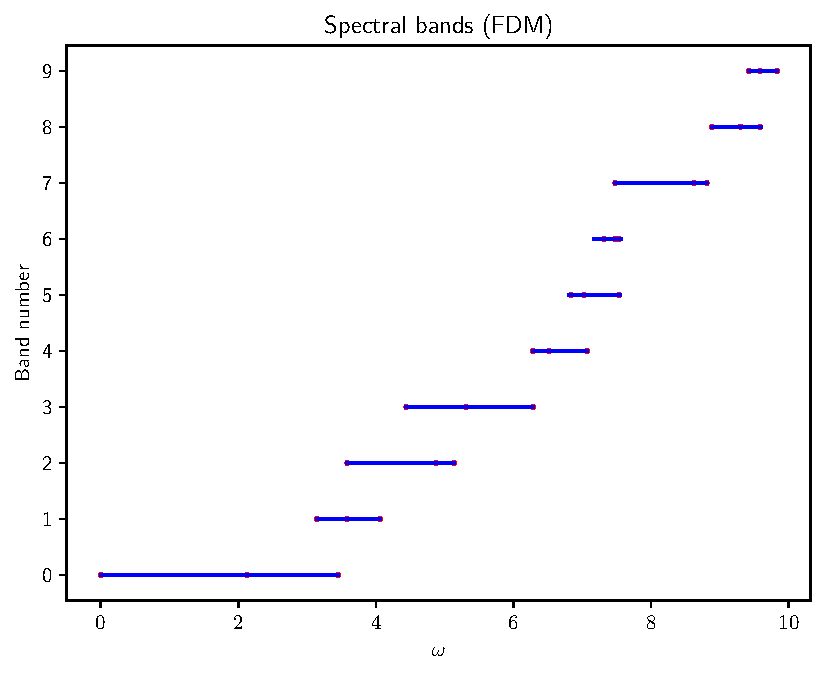
\includegraphics[scale=0.45]{CompositeCross-FDM-SpectralBands-alpha0.pdf}
		\caption[]{\label{fig:CompositeCross-FDM-SpectralBands-alpha0} Spectral bands when $\alpha=0$.}
	\end{subfigure}
	~
	\begin{subfigure}[t]{0.45\textwidth}
		\centering
		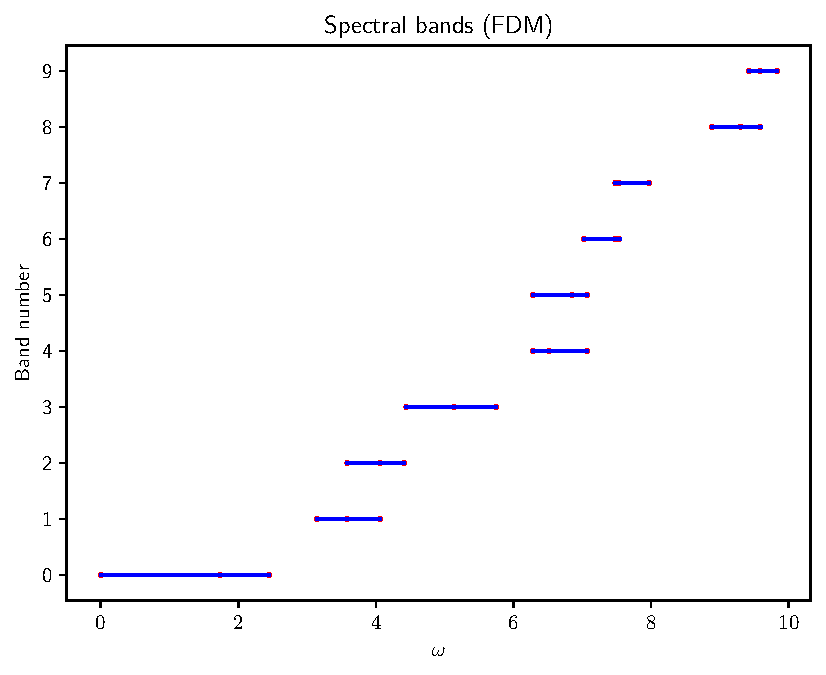
\includegraphics[scale=0.45]{CompositeCross-FDM-SpectralBands-alpha1.pdf}
		\caption[]{\label{fig:CompositeCross-FDM-SpectralBands-alpha1} Spectral bands when $\alpha=1$.}
	\end{subfigure}
	\caption[Spectral bands of \eqref{eq:SI-WaveEqn}, computed via solution of the problem \eqref{eq:SI-StrongForm}.]{\label{fig:CompositeCross-FDM-SpectralBands} The approximate eigenvalues computed by the finite-difference scheme, sorted into spectral bands for the cross-in-the-plane geometry. Eigenvalues corresponding to the extremities of the quasi-momentum are plotted in red.}
\end{figure}
Those points plotted in red correspond to eigenvalues that were computed at quasi-momentum values of $\bracs{0,0}^\top$, $\bracs{-\pi,0}^\top$, $\bracs{0,-\pi}^\top$, $\bracs{-\pi,-\pi}^\top$, from which we can observe that these points typically form the endpoints of each of the spectral bands.
Much like the quantum graph case, we do not expect this to occur for general geometries --- there even appears to be a notable example of this in band 6, for which the eigenvalues at the extremities of the band are not obtained at any of these quasi-momentum values.
However by examining the eigenvalues in this band as functions of $\qm$, as in figure \ref{fig:FDM_2022-01-28-09-33_AllBands}, it can be noticed that these extreme eigenvalues occur at quasi-momentum values where one of the components is either 0 (for the minimum values) or $-\pi$ (for the maximum values).
\begin{figure}[b!]
	\centering
	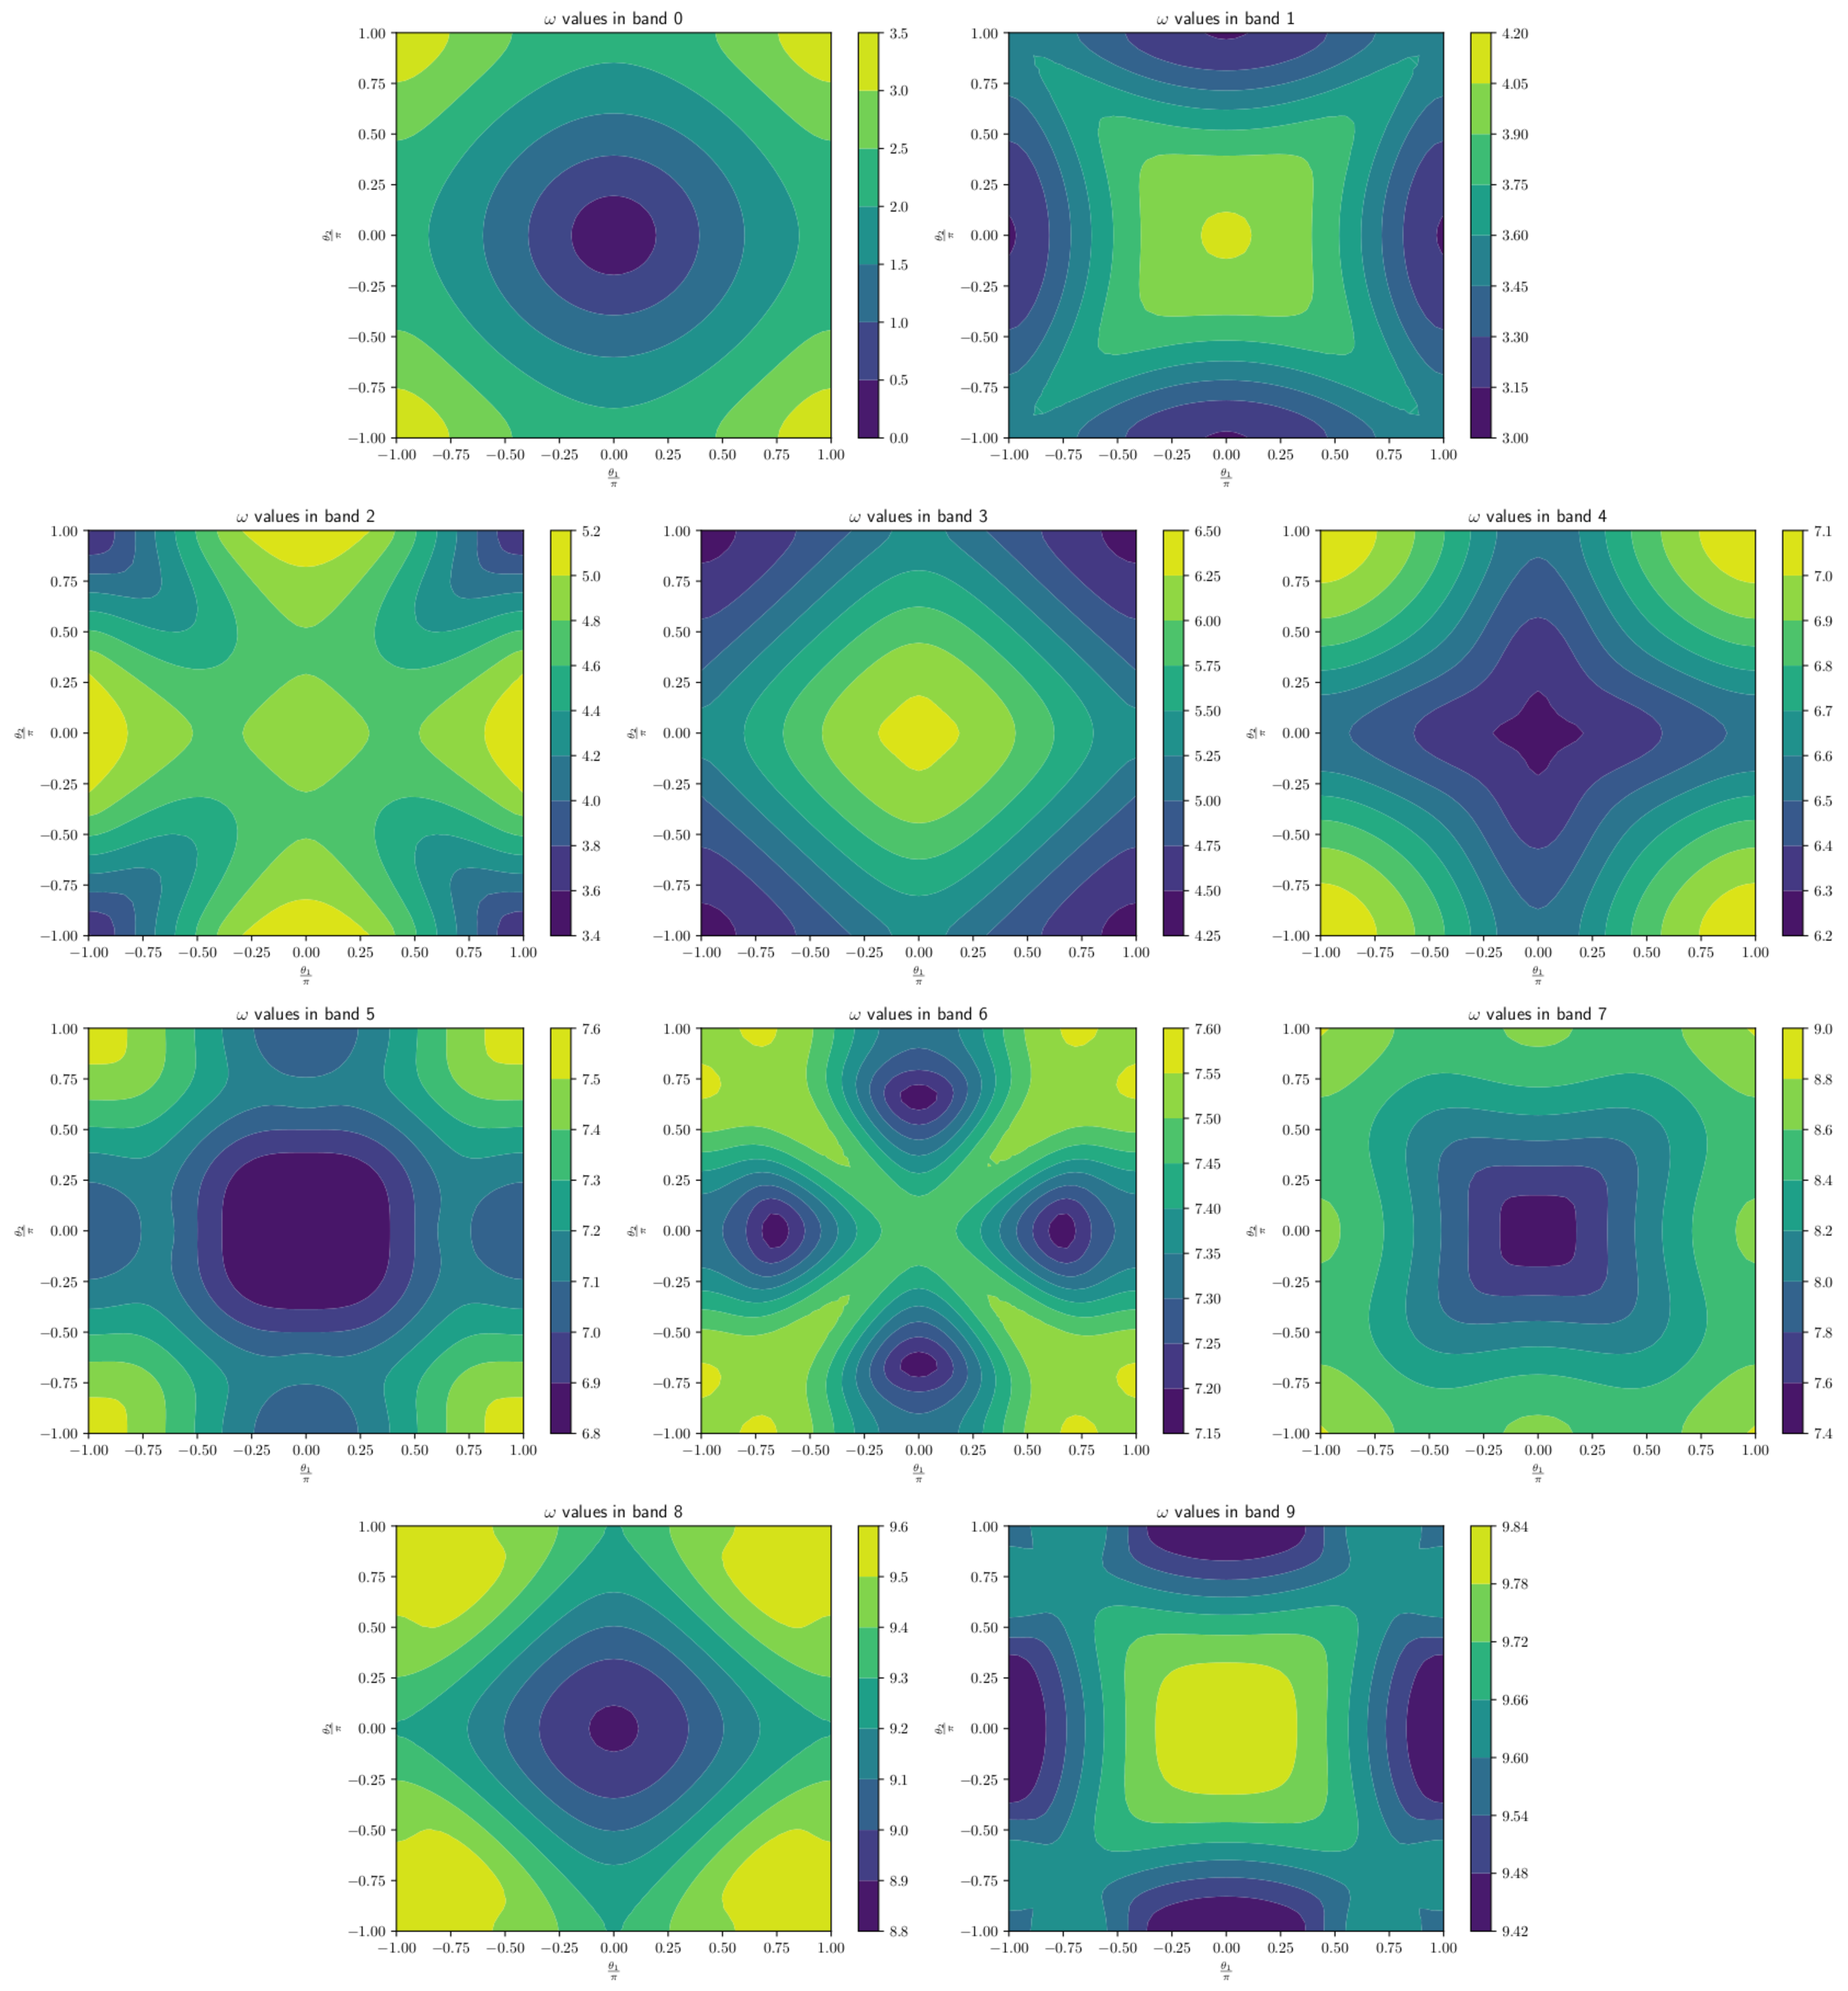
\includegraphics[width=\textwidth]{FDM_2022-01-28-09-33_AllBands.pdf}
	\caption[Dispersion relations for the first 10 spectral bands of \eqref{eq:SI-WaveEqn}, computed via solution of \eqref{eq:SI-StrongForm} with $\alpha=0$.]{\label{fig:FDM_2022-01-28-09-33_AllBands} The eigenvalues $\omega$ in each spectral band, plotted as functions of the quasi-momentum $\qm$. Observe the symmetries that are expected from proposition \ref{prop:CrossInPlaneSymmetries}.}
\end{figure}
Similarly to our approach via \eqref{eq:SI-VarProb}, the eigenvalues within each band obey the symmetries expected from proposition \ref{prop:CrossInPlaneSymmetries}.
We also note that the presence of non-zero $\alpha$, that is \emph{geometric contrast} in our material, has been sufficient to open spectral gaps.
We additionally note that the Dirichlet eigenvalues $\omega_{n,m}^2=\bracs{n^2+m^2}\pi^2$ remain a part of the spectrum, as expected (since the corresponding eigenfunctions have $u_{n,m}(v_j)=0$).

A distinct advantage of using this method over that for solving problem \ref{prob:DiscVarProb} is that, once the finite difference matrix $\mathcal{F}$ is assembled, we can use matrix-eigenvalue solvers to examine the eigenvalues near to any positive number that we choose, without needing to compute \emph{all} the previous eigenvalues (and eigenfunctions) up to this value.
This allows us to easily test the rate of convergence of the numerical scheme to the eigenvalues $\omega_{n,m}^2 = \bracs{n^2+m^2}\pi^2$.
In these cases, we expect that the error in the approximate eigenvalue is of the order of $N^{-2}$, since our scheme makes use of centred differences in the bulk region, and on the skeleton the eigenfunction should be identically zero.
This is what we observe numerically, and is illustrated in figure \ref{fig:CompositeCross-FDM-DEV} for $n\leq m\in\clbracs{1,2,3}$ (the cases $n>m$ are similar due to the aforementioned symmetry).
\begin{figure}[b!]
	\centering
	\begin{subfigure}[t]{0.45\textwidth}
		\centering
		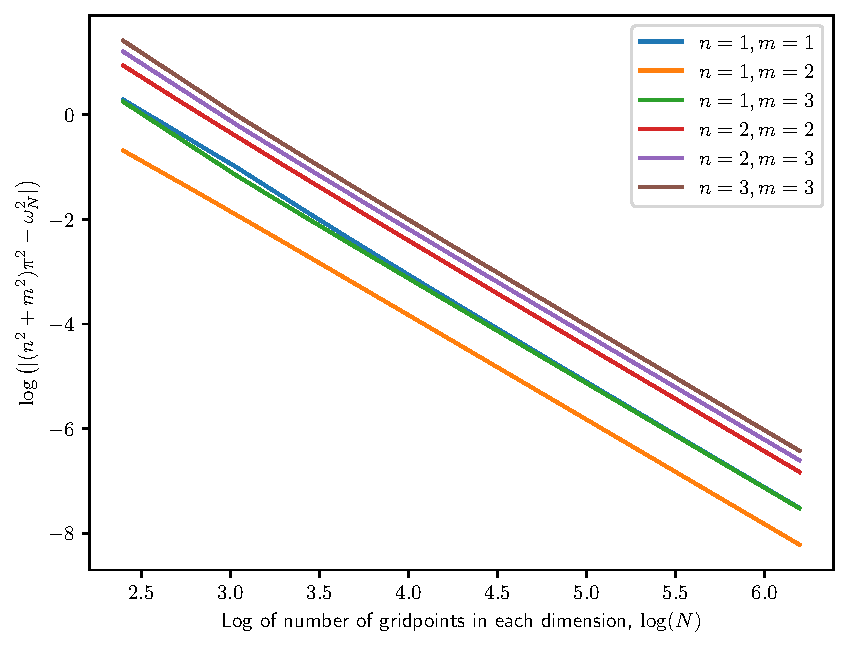
\includegraphics[scale=0.45]{CompositeCross-FDM-DEV-LogError.pdf}
		\caption[]{\label{fig:CompositeCross-FDM-DEV-LogError} Logarithm of the error in the eigenvalue against $\log(N)$, for a selection of $n,m$ values.}
	\end{subfigure}
	~
	\begin{subfigure}[t]{0.45\textwidth}
		\centering
		\begin{tabular}[b]{| c | c | c |}
			\hline
			$\bracs{n,m}$ & Intercept & Gradient \\
			\hline
			$\bracs{1, 1}$ & $5.14236963$ & $-2.04617746$ \\
			\hline
			$\bracs{1, 2}$ & $4.14218510$ & $-1.99442370$ \\
			\hline
			$\bracs{1, 3}$ & $4.96573274$ & $-2.01780686$ \\
			\hline
			$\bracs{2, 2}$ & $5.70851785$ & $-2.02509086$ \\
			\hline
			$\bracs{2, 3}$ & $5.95893392$ & $-2.03031478$ \\
			\hline
			$\bracs{3, 3}$ & $6.14879571$ & $-2.03187802$ \\
			\hline
		\end{tabular}
		\caption[]{\label{fig:CompositeCross-FDM-DEV-LoBF} Line of best fit (via least squares regression) for each pair $\bracs{n,m}$.}
	\end{subfigure}
	\caption[Error in the eigenvalue approximation as a function of mesh size, for the cross-in-the-plane geometry.]{\label{fig:CompositeCross-FDM-DEV} Convergence rate for the FDM method to the analytic eigenvalues shared with the Dirichlet laplacian. Observe that the estimated gradient, hence convergence rate with $N$, is approximately $-2$ as expected.}
\end{figure}
Regrettably, we do not have to hand any analytic solutions to \eqref{eq:SI-WaveEqn} beyond those shared with the Dirichlet laplacian and so we cannot test the rate of convergence for solutions which are non-constant along the skeleton.

Our example using the cross-in-the-plane geometry illustrates the principle behind this approach; use finite differences to approximate $u$ in each $\ddom_i$ and along each $I_{jk}$, and tie approximations from adjacent bulk regions together through the nodal values along the common edge of the skeleton.
Compared to the variational approach in section \ref{sec:SI-VarProbMethod}, this approach avoids working with $\ccompMes$ directly and instead allows us to work solely in terms of classical derivatives, approximating them through Taylor's theorem.
However by choosing to approximate our function within each region and then ``stitch" these approximations together, we must choose our mesh in such a way as to abide by this decision, which can lead to some further considerations.
Let us begin by considering the requirements of the placement of nodes within the bulk regions --- each node must have neighbours in each of the coordinate directions that lie within the (closure of) the bulk region.
Now, consider a bulk region like that in figure \ref{fig:Diagram_FDMMeshIssue}, where a part of the skeleton is not aligned to the coordinate axes.
\begin{figure}[t]
	\centering
	\begin{subfigure}[t]{0.3\textwidth}
		\centering
		\includegraphics[scale=1.0]{Diagram_FDMMeshIssue-a.pdf}
		\caption[]{\label{fig:Diagram_FDMMeshIssue-a} A uniform mesh does not ensure that nodes in the bulk regions have neighbouring nodes which will provide us with a $C^2$-approximation, nor that every vertex has a node placed at it.}
	\end{subfigure}
	~
	\begin{subfigure}[t]{0.3\textwidth}
		\centering
		\includegraphics[scale=1.0]{Diagram_FDMMeshIssue-b.pdf}
		\caption[]{\label{fig:Diagram_FDMMeshIssue-b} Placing additional nodes along the skeleton edges, ensuring nodes in the bulk region have neighbours that lie within that same bulk region or on its boundary.}
	\end{subfigure}
	~
	\begin{subfigure}[t]{0.3\textwidth}
		\centering
		\includegraphics[scale=1.0]{Diagram_FDMMeshIssue-c.pdf}
		\caption[]{\label{fig:Diagram_FDMMeshIssue-c} The nearest nodes in the directions $\pm n_{jk}$ from the skeleton may be far from the edge or not exist at all (left highlighted node). Interpolation (right highlighted node) offers a solution, provided the bulk region is meshed well.}
	\end{subfigure}
	\caption[Considerations for the placement of mesh nodes when handling arbitrary skeleton geometries.]{\label{fig:Diagram_FDMMeshIssue} An illustration of the complications encountered and considerations to be made when setting up a finite difference based approach for a general skeleton.}
\end{figure}
As we can quickly realise, uniform mesh will not be sufficient in this case, nor in general when the skeleton has edges that are not aligned to the coordinate axes. 
In figure \ref{fig:Diagram_FDMMeshIssue-a}, the highlighted node in the bulk region has no neighbour ``below" that lies within the same bulk region or its boundary, so a centred difference approximation to $\laplacian_{\qm}u$ at this node cannot be used.
One could argue that a suitable value for $u$ ``below" the highlighted node could be read off from interpolating values between nodes along the edge (then applying the knowledge that $u$ is continuous across the skeleton).
However there is no assurance that this interpolation will produce an accurate value for $u$, particularly if we are in the situation in figure \ref{fig:Diagram_FDMMeshIssue-a} where there are only two nodes along the diagonal edge, and the lower-left vertex doesn't even have a node placed at it.
To address this meshing complication, one can introduce additional nodes along the skeleton (and at the vertices) where necessary, as in figure \ref{fig:Diagram_FDMMeshIssue-b} (highlighted in blue).
This results in every node in the bulk regions having suitable neighbours in the coordinate directions, and has the additional bonus of improving the approximation of the derivative of $u$ along the skeleton.
Our expense is that we have given up a uniform distance between all nodes, which will require us to take slightly care when deriving difference equations at each node and assembling the matrix $\mathcal{F}$, and the rate of convergence will likely scale with some power of the \emph{greatest} such inter-nodal distance.

We also may end up compounding another issue when we come to approximate the normal derivative traces in \eqref{eq:SI-FDMSkeleton}, which we highlight in figure \ref{fig:Diagram_FDMMeshIssue-c} --- if an edge is not aligned with the coordinate axes, where are the nearest nodes in the directions $\pm n_{jk}$ from the edge?
There is the possibility that such a node is far from the edge, again resulting in a poor approximation to the trace of the normal derivative, or that such a node may not even exist (see the leftmost highlighted node in figure \ref{fig:Diagram_FDMMeshIssue-c}).
We again have the option of interpolating a value for $u$ in the bulk regions, schematically illustrated at the right highlighted node in figure \ref{fig:Diagram_FDMMeshIssue-c} --- the values at the orange points can be interpolated from nodes in the bulk region, provided we have already made sensible mesh choices within the adjacent bulk regions\footnote{Note that we cannot simply decide to make the mesh in the bulk region finer, so that a node is placed in the position we want to interpolate. In general, doing so will end up in us requiring more nodes on the skeleton through the issue in figure \ref{fig:Diagram_FDMMeshIssue-a}, sending us in circles!}.
These issues arise due to how the skeleton (or more precisely, each edge of the skeleton) is effectively using a different coordinate system (for its derivatives) to the bulk regions, which is why this issue disappears when the edges of the skeleton are aligned to the coordinate axes --- the ``neighbouring" nodes we need on the skeleton are in the directions $e_{jk}, n_{jk}$ rather than the coordinate directions $x_1, x_2$.
Whilst the complications this brings can be combatted in the manners discussed above, it does highlight the need for care when setting up and implementing this approach for general skeleton geometries.
Contrastingly, the approach via \eqref{eq:SI-VarProb} does not run into these issues since (in that approach) we have made the choice to work with $\ccompMes$ directly and approximate the related gradients globally (over the whole domain) rather than utilising their properties on sub-regions.

% Ideas for numerical solution of the problem
%\section{Numerical Approach to the Variational Problem and Strong Formulation} \label{sec:SI-VPandFDM}
\tstk{fix this section's name once you decide what makes the cut. Also make a proper introduction here, or at least a lead-in.}

In this section we turn to numerical schemes for handling the variational problem \eqref{eq:SI-VarProb} and the strong formulation \eqref{eq:SI-BulkEqn}-\eqref{eq:SI-VertexCondition}.
For each formulation, we will outline the numerical scheme we have chosen to pursue and, importantly, the methods in which we can handle the non-standard integrals and gradients with respect to $\compMes$ numerically.
Where appropriate we will use the "cross-in-the-plane" geometry from the example in section \tstk{ref!!}, now equipped with $\compMes$, to illustrate the results of these methods.

\subsection{Variational Problem} \label{ssec:SI-VP}
We begin by examining the variational problem \eqref{eq:SI-VarProb},
\begin{align*} 
	\omega_n^2 &:= \min_{u}\clbracs{ \integral{\ddom}{ \abs{\tgrad_{\compMes}u}^2 }{\compMes} \setVert \norm{u}_{\ltwo{\ddom}{\compMes}}=1, \ u\perp u_l \ \forall 1\leq l\leq n-1 }. \tag{\eqref{eq:SI-VarProb} restated}
\end{align*}
Our interest is in determining the eigenvalues $\omega_n^2$, however we also need to determine the eigenfunctions $u_n$ since we need $u_n$ to be orthogonal to each of $u_l, 1\leq l\leq n-1$.
Given that we can obtain the eigenvalue $\omega_n^2$ from the eigenfunction $u_n$ by evaluating the integral in \eqref{eq:SI-VarProb}, we will focus our discussion on the approximation (and computation) of the eigenfunctions.
We also drop the explicit subscript $n$, and just consider the problem of determining the function $u\in\tgradSob{\ddom}{\compMes}$ which solves the optimisation problem
\begin{subequations} \label{eq:SI-MinProblem}
	\begin{align}
		\text{Minimise} \quad & \quad \integral{\ddom}{ \abs{\tgrad_{\compMes}u}^2 }{\compMes} \\
		\text{Subject to} \quad & \quad \integral{\ddom}{ \abs{u}^2 }{\compMes} = 1, \\
		& \quad \integral{\ddom}{ u\cdot\overline{u}_l }{\compMes} = 0, \ 1\leq l\leq n-1,
	\end{align}
\end{subequations}
where $n\in\naturals$, $u_l, 1\leq l\leq n-1$ are given (pairwise) orthogonal functions.
The traditional idea when attempting to approximate a minimising function is to represent the minimising function $u$ in a basis $\clbracs{\varphi_m}_{m\in\naturals_0}\subset\tgradSob{\ddom}{\compMes}$, truncate the basis expansion at some index $M$,
\begin{align} \label{eq:SI-VPTruncatedBasis}
	u &\approx \sum_{m=0}^M u_m \varphi_m,
\end{align}
and solve the minimisation problem (that arises from substituting \eqref{eq:SI-VPTruncatedBasis} into \eqref{eq:SI-MinProblem}) in the coefficients of the basis expansion that remain --- the choice of $M$ determines the accuracy in the approximate eigenfunction (and hence eigenvalue).
This minimisation problem will be discrete (solving for the $M+1$ independent variables $u_m$), and can be handled using optimisation methods.

None of the steps above are prohibited for the problem \eqref{eq:SI-MinProblem}, and so we can proceed with the aforementioned ideas.
We will illustrate this implementation for the "cross-in-the-plane" geometry first introduced in \tstk{example reference}\footnote{For convenience, we have translated the period cell by $\bracs{\recip{2},\recip{2}}$ with regards to how this geometry was handled in \tstk{ref}. This just allows us to avoid carrying additional constant terms around in our computations, and we would obtain the same results as if we didn't apply any translation.}; we take $\ddom=\left[0,1\right)^2$, and let $\graph$ be the period graph with a single vertex $v_0=\bracs{0,0}^\top$, and two ``looping" edges $I_h = \sqbracs{0,1}\times\clbracs{0}$, $I_v=\clbracs{0}\times\sqbracs{0,1}$.
Our first task is to decide on the basis functions $\varphi_m$ that we want to use to approximate $u$.
From the standpoint of accuracy (and typically speed) of the numerical solution there are several properties that it is desirable for this basis to have; orthonormality between the $\varphi_m$, similar shape to that expected of $u$, and of course periodicity.
This is where problems concerning the unfamiliar nature of our space $\tgradSob{\ddom}{\compMes}$ begin to arise, as the choice of basis is considerably more complex --- as choosing the behaviour of $\varphi_m$ in the bulk regions then restricts what $\varphi_m$ can do on the skeleton, and vice-versa. 
The geometry of the skeleton can also compound this issue, particularly if there are a large number of bulk regions $\ddom_i$, if they have irregular shapes, or if their shapes are significantly different (in terms of size or shape) from each other.
As a general approach, one can choose a basis in similar fashion to how this is done for finite element schemes; mesh $\ddom$ into a union of simplexes (usually triangles) by placing nodes $\tau_i$, ensuring that none of the simplexes straddle any parts of the skeleton (that is, the interior of a simplex never has non-empty intersection with part of the skeleton).
Then, use ``tent" or ``hat" functions centred on each node $\tau_i$ for the truncated basis functions $\varphi_m$.
This allows sufficient flexibility in the behaviour of $u$ on the edges and in the bulk regions, at the expense of requiring a new mesh for every new graph geometry.

Fortunately, the geometry of our ``cross-in-the-plane" example is rather simple, since the two edges $I_h, I_v$ are aligned with the coordinate axes.
This makes computing integrals on the skeleton much simpler, and traces from the bulk region can be computed with relative ease, so we can avoid taking the approach of meshing $\ddom$ as described above.
Instead, we can opt to choose a basis in a way more akin to spectral methods --- by choosing ``global" basis functions rather than the ``local" tent-basis functions that meshing $\ddom$ would utilise.
Combined with the fact that we only have one bulk region that spans the entire period cell, the natural candidate for our basis functions would be the 2D Fourier basis $\e^{2\pi\rmi(\alpha x + \beta y)}$.
These functions are orthogonal in $\ltwo{\ddom}{\compMes}$, have period cell $\ddom$, and on each of the edges of $\graph$ reduce to a 1D-Fourier series.
However, these functions also possess a continuous (in the sense of matching traces) normal derivative across the skeleton, which functions in $\tgradSob{\ddom}{\compMes}$ are not required to have, and so we cannot use the Fourier basis.
Instead, we will look to use 2D polynomials to approximate our function $u$, by taking $M\in\naturals$ and setting
\begin{align} \label{eq:2DPolyBasisDef}
	\varphi_m(x,y) &= x^{i_m} y^{j_m}, \quad m = j_m + Mi_m, \ i,j\in\clbracs{0,...,M-1}.
\end{align}
These functions are not periodic by definition, so we are required to add the additional constraints
\begin{align*}
	u\bracs{0,y} = u\bracs{1,y}, \ \forall y\in\sqbracs{0,1}, 
	\qquad 
	u\bracs{x,0} = u\bracs{x,1}, \ \forall x\in\sqbracs{0,1},
\end{align*}
to our minimisation problem to account for this.
With this choice of basis, and writing $U = \bracs{u_0,...,u_{M^2-1}}^\top$, we are tasked with solving the following problem.
\begin{problem}[Discrete Variational Problem] \label{prob:DiscVarProb}
	Let $M,N\in\naturals$ and $\varphi_m$ be as in \eqref{eq:2DPolyBasisDef}.
	Given coefficients $U_l=\bracs{u^l_0,...,u^l_{M^2-1}}^\top$ for $1\leq l\neq N-1$, find values $U=\bracs{u_0,...,u_{M^2-1}}^\top$ that:
	\begin{subequations} \label{eq:SI-ExampleMinProb}
		\begin{align}
			\text{Minimise} \quad & \quad J\sqbracs{U} := \sum_{m=0}^{M^2-1}\sum_{n=0}^{M^2-1}u_m\overline{u}_n\ip{\tgrad_{\compMes}\varphi_m}{\tgrad_{\compMes}\varphi_n}_{\ltwo{\ddom}{\compMes}^2} 
			\label{eq:SI-EMPObjectiveFn} \\
			\text{Subject to} \quad & \quad \sum_{m=0}^{M^2-1}\sum_{n=0}^{M^2-1}u_m\overline{u}_n\ip{\varphi_m}{\varphi_n}_{\ltwo{\ddom}{\compMes}} = 1, 
			\label{eq:SI-EMPNormConstraint} \\
			& \quad \sum_{i_m=1}^{M-1}u_{j_m+Mi_m} = 0, \ \forall j_m\in\clbracs{0,...,M-1}, 
			\label{eq:SI-EMPxPeriodicity} \\
			& \quad \sum_{j_m=1}^{M-1}u_{j_m+Mi_m} = 0, \ \forall i_m\in\clbracs{0,...,M-1},
			\label{eq:SI-EMPyPeriodicity} \\
			& \quad \sum_{m=0}^{M^2-1}\sum_{n=0}^{M^2-1}u_m\overline{u}^l_n\ip{\varphi_m}{\varphi_n}_{\ltwo{\ddom}{\compMes}} = 0, \ \forall 1\leq l\leq N-1.
			\label{eq:SI-EMPOrthogonality}
		\end{align}
	\end{subequations}
\end{problem}
The minimiser $U$ of problem \ref{prob:DiscVarProb} then provides our approximation of $u$, and we have that $\omega^2 \approx J[U]$.
Equation \eqref{eq:SI-EMPNormConstraint} is the norm constraint on the eigenfunction $u$, \eqref{eq:SI-EMPxPeriodicity} (respectively \eqref{eq:SI-EMPyPeriodicity}) are the constraints that ensure periodicity of the eigenfunction in the $x$ (respectively $y$) directions, and \eqref{eq:SI-EMPOrthogonality} forces $u$ to be orthogonal to the previously computed eigenfunctions $u^l$.
Due to the finite dimension of our problem (through the truncation at order $M$ for the functions $\varphi_m$), we are only ever able to compute approximations to the lowest $M^2 - \bracs{2M + 1} + 1$ eigenvalues due to the number of constraints in the problem \ref{prob:DiscVarProb}.

\tstk{time to display some nice figures, maybe some comparisons between the two methods etc? Could also do a run of this with $\alpha_3\neq0$ just to see what on earth happens!}

\subsection{Finite Difference Scheme} \label{ssec:FDMSingInc}
\tstk{This is the content summary of \texttt{CompositeMedium\_PeriodicFDM.ipynb}}
As an alternative to working directly from the variational problem \ref{prob:DiscVarProb}, we can instead choose to work from our ``strong formulation" \eqref{eq:SI-BulkEqn}-\eqref{eq:SI-VertexCondition}.
Before we do so, it is convenient to notice that we can move the ``trace" terms in \eqref{eq:SI-InclusionEqn} to the left-hand-side to obtain the slightly nicer (in terms of the numerics that follow) looking system
\begin{subequations} \label{eq:SI-FDMEquationsToDisc}
	\begin{align}
		-\laplacian_\qm u 
		&= \omega^2 u 
		&\text{in } \ddom_i, \label{eq:SI-FDMBulk} \\
		- \bracs{\diff{}{y} + \rmi\qm_{jk}}^2u^{(jk)}  - \bracs{\bracs{\grad u\cdot n_{jk}}^+ - \bracs{\grad u\cdot n_{jk}}^-}
		&= \omega^2 u^{(jk)},
		&\text{in } I_{jk}, \label{eq:SI-FDMSkeleton} \\
		\sum_l \bracs{\pdiff{}{n}+\rmi\qm_{jk_l}} u^{(jk_l)}(v_j) 
		&= 0 
		&\text{at } v_j\in\vertSet. \label{eq:SI-FDMVertex}
	\end{align}
\end{subequations}
We have now placed everything except terms involving the spectral parameter on the left hand side of \eqref{eq:SI-FDMEquationsToDisc}, and our goal now is to devise a numerical scheme to approximate the action of the ``operators" on the left-hand-side, and from that approximate the spectrum of the problem.

Our idea is as follows; we recognise that $u$ is twice differentiable (in the familiar, classical sense) in each of the bulk regions and along each of the skeleton edges, so we can look to to approximate the spectrum of our problem by approximating $u$ through a (somewhat n{\"i}ave) finite-difference approximation in each of the bulk regions and skeleton edges, and tying these ``region-wise" approximations together.
To this end, we take each of the bulk regions $\ddom_i$, and place nodes $\tau_j\in\overline{\ddom}_{i}$ appropriately, so as to write finite difference approximations for $\laplacian_{\qm}u$ at each node $\tau_j\in\ddom_i$.
Note that, since $u$ is not required to be differentiable (in the classical sense) across the skeleton, it is important that any finite difference approximation at $\tau_j$ only uses the values of $u$ at other nodes in $\overline{\ddom}_{i}$.
In placing nodes in $\overline{\ddom}_{i}$, we will also end up with nodes placed on the portion of the skeleton (and vertices) that form part of $\partial\ddom_i$.
Since $u$ is twice differentiable along the skeleton, the placement of these nodes allows us to derive finite-difference approximations for the derivatives in \eqref{eq:SI-FDMSkeleton}.
The traces of the normal derivates (in \eqref{eq:SI-FDMSkeleton}) can also be approximated via one-sided differences using suitable nodes from each of the adjacent bulk regions.
Finally, an approximation for \eqref{eq:SI-FDMVertex} can be derived for nodes that lie at vertices $v_j\in\vertSet$, using the nodes that lie on edges that connect to $v_j$.
We will come to highlight some of the difficulties with this procedure \tstk{where?}, but assuming we have approximations for the gradient- and derivative-like objects, we can then approximate the action of the left-hand-side of \eqref{eq:SI-FDMEquationsToDisc} via the action of a matrix $\mathcal{F}$ on the vector $U = \bracs{u_j}^\top$, where $u_j:=u\bracs{\tau_j}$.
As a result, we can then approximate the system \eqref{eq:SI-FDMEquationsToDisc} by the matrix-eigenvalue problem involving $\mathcal{F}$.

\tstk{once you have the plots ready, rephrase this to something like ``we will begin by demonstrating this idea for the X-in-plane geometry, and it's coincidence with the results from the previous VP method".}
Let us begin by illustrating this approach using the ``Cross in the plane" geometry \tstk{section ref}.
We first discretise $\ddom$ into a uniform mesh consisting of $N\times N$ nodes $\tau_{p,q} = \bracs{(p-1)h,(q-1)h}$ for $p,q\in\clbracs{1,...,N}$, with a mesh width of $h = \recip{N-1}$, and write $u_{p,q} = u\bracs{\tau_{p,q}}$.
It is important to note at this early stage that we can utilise a uniform mesh thanks to the rather simple geometry of the skeleton, and in general the meshing process will be more complex (which we will address \tstk{where? soon? after this description?})
Note that there is no need to place nodes along both of the periodic edges of $\ddom$, so long as we keep track of which nodes are connected by periodicity, but for notational purposes it is convenient to include such nodes in our description.
Proceeding with the discretisation of the above equations, $u$ is twice differentiable in the bulk region $\ddom^{\circ}$, and so at points $\tau_{p,q}\not\in\graph$ we can discretise as
\begin{align*}
	-\laplacian_\qm u\bracs{\tau_{p,q}} &\approx 
	\bracs{\abs{\qm}^2 + 4h^{-2}}u_{p,q}
	-h^{-1}\bracs{h^{-1} + \rmi\qm_1}u_{p+1,q}
	-h^{-1}\bracs{h^{-1} - \rmi\qm_1}u_{p-1,q} \\
	&\qquad -h^{-1}\bracs{h^{-1} + \rmi\qm_2}u_{p,q+1}
	-h^{-1}\bracs{h^{-1} - \rmi\qm_2}u_{p,q-1}, \labelthis\label{eq:SI-FDMBulkDiscretise}
\end{align*}
using centred differences.
One can also use forward (also known as left) or backward (a.k.a right) differences to approximate the $\laplacian_{\qm}$ operator --- this will likely be necessary for more complex skeleton geometries as was hinted at previously.
Also worth noting is that, should one choose not to use (or be unable to use) a uniform mesh, one will still obtain a similar expression to \eqref{eq:SI-FDMBulkDiscretise} for the approximation of $\laplacian_\qm u$ at a node $\tau\not\in\graph$, but in terms of the values of $u$ at, and the distances to, the ``nearest neighbour" nodes to $\tau$.

For nodes $\tau_{p,q}\in I_{jk}$ (for either $I_{jk}=I_h$ or $I_v$), our finite difference approximations become slightly more complex as we are forced to consider the nearest nodes to $\tau_{p,q}$ that lie in the directions $e_{jk}$ and $n_{jk}$.
This is because $u$ is twice differentiable \emph{along the skeleton}, so we must approximate $\bracs{\diff{}{y} + \rmi\qm_{jk}}^2u^{(jk)}$ through finite differences along the edge $I_{jk}$, which will involve the values of $u$ at the nodes ``adjacent" to $\tau_{p,q}$ in the $e_{jk}$ and $-e_{jk}$ directions.
For the normal-derivative trace terms, we use one-sided finite differences to approximate these values at $\tau_{p,q}$, which involves the values of $u$ at the nodes ``adjacent" to $\tau_{p,q}$ in the $n_{jk}$ and $-n_{jk}$ directions.
In general, these requirements will contribute to the complications with meshing the domain as discussed in \tstk{where?!}, but since the edges are aligned with the coordinate axes in the cross-in-the-plane geometry, the vectors $e_{jk}$ and $n_{jk}$ are also aligned with the coordinate axes and the discretisation proceeds easily.
Those $\tau_{p,q}$ that lie on the horizontal edge $I_h$ have $q=\frac{N-1}{2}$ and $p\neq\frac{N-1}{2}$, so our finite difference approximation is
\begin{align*}
	- \bracs{\diff{}{y} + \rmi\qm_{jk}}^2u_{p,q} - \bracs{\bracs{\grad u_{p,q}\cdot n_{jk}}^+ - \bracs{\grad u_{p,q}\cdot n_{jk}}^-}
	& \approx \bracs{\qm_1^2 + 2h^{-1} + 2h^{-2}}u_{p,q} \\
	& \quad - h^{-1}\bracs{h^{-1} + \rmi\qm_1}u_{p+1,q} \\
	& \quad - h^{-1}\bracs{h^{-1} - \rmi\qm_1}u_{p-1,q} \\
	& \quad - h^{-1}u_{p,q+1} - h^{-1}u_{p,q-1}, \labelthis\label{eq:SI-FDMHorzEdgeDiscretise}
\end{align*}
(where we reiterate $q=\frac{N-1}{2}$ and $p\neq\frac{N-1}{2}$).
Here we have used centred differences along the edge $I_h$, identifying that the nodes $\tau_{p-1,q}, \tau_{p+1,q}$ are the adjacent nodes in the $x_1 (= e_h)$ direction.
The traces cause the introduction of the terms $u_{p,q-1}$ and $u_{p,q+1}$, since $-x_2 = n_h$.
Analogously, nodes $\tau_{p,q}$ on the vertical edge $I_v$ have $p=\frac{N-1}{2}$ and $q\neq\frac{N-1}{2}$, and the finite difference approximation is
\begin{align*}
	- \bracs{\diff{}{y} + \rmi\qm_{jk}}^2_{p,q} - \bracs{\bracs{\grad u_{p,q}\cdot n_{jk}}^+ - \bracs{\grad u_{p,q}\cdot n_{jk}}^-}
	& \approx \bracs{\qm_2^2 + 2h^{-1} + 2h^{-2}}u_{p,q} \\
	& \quad - h^{-1}\bracs{h^{-1} + \rmi\qm_2}u_{p,q+1} \\
	& \quad - h^{-1}\bracs{h^{-1} - \rmi\qm_2}u_{p,q-1} \\
	& \quad - h^{-1}u_{p+1,q} - h^{-1}u_{p-1,q}. \labelthis\label{eq:SI-FDMVertEdgeDiscretise}
\end{align*}

Finally, we come to the node $\tau_{\frac{N-1}{2},\frac{N-1}{2}}$ placed at the vertex $v_0$.
Our finite difference approximation already enforces that $u$ be continuous at $v_0$, so we just have to enforce the vertex condition at this node.
Here we again approximate each (signed) normal derivative by a one-sided finite difference from the adjacent edges, giving us
\begin{align} \label{eq:SI-FDMVertCond}
	\sum_{j\con k}\bracs{ \pdiff{}{n} + \rmi\qm_{jk} }u_{\frac{N-1}{2},\frac{N-1}{2}}
	&\approx h^{-1} \bracs{ 4u_{p,q} - u_{p+1,q} - u_{p-1,q} - u_{p,q+1} - u_{p,q-1} },
\end{align}
where $p = q = \frac{N-1}{2}$.
We now insert these finite difference approximations \eqref{eq:SI-FDMBulkDiscretise}-\eqref{eq:SI-FDMVertCond} into \eqref{eq:SI-FDMEquationsToDisc}, which provides the following system in the $\bracs{N-1}^2$ nodal values $u_{p,q}$;
\begin{subequations} \label{eq:SI-FDMDiscreteEqns}
	\begin{align*}
		\bracs{\abs{\qm}^2 + 4h^{-2}}u_{p,q} \\
		-h^{-1}\bracs{h^{-1} + \rmi\qm_1}u_{p+1,q}
		-h^{-1}\bracs{h^{-1} - \rmi\qm_1}u_{p-1,q} & & \\
		\quad -h^{-1}\bracs{h^{-1} + \rmi\qm_2}u_{p,q+1}
		-h^{-1}\bracs{h^{-1} - \rmi\qm_2}u_{p,q-1}
		& = \omega^2 u_{p,q}, &\quad p,q\neq\frac{N-1}{2}, \labelthis\label{eq:SI-FDMBulkDiscEqns} \\
		\bracs{\qm_1^2 + 2h^{-1} + 2h^{-2}}u_{p,q} \\
		- h^{-1}\bracs{h^{-1} + \rmi\qm_1}u_{p+1,q}
		- h^{-1}\bracs{h^{-1} - \rmi\qm_1}u_{p-1,q} & & \\
		\quad - h^{-1}u_{p,q+1} - h^{-1}u_{p,q-1}
		&= \omega^2 u_{p,q}, &\quad p\neq\frac{N-1}{2}, q=\frac{N-1}{2}, \labelthis\label{eq:SI-FDMHEdge} \\
		\bracs{\qm_2^2 + 2h^{-1} + 2h^{-2}}u_{p,q} \\
		- h^{-1}\bracs{h^{-1} + \rmi\qm_2}u_{p,q+1}
		- h^{-1}\bracs{h^{-1} - \rmi\qm_2}u_{p,q-1} & & \\
		- h^{-1}u_{p+1,q} - h^{-1}u_{p-1,q}
		&= \omega^2 u_{p,q}, &\quad p=\frac{N-1}{2}, q\neq\frac{N-1}{2}, \labelthis\label{eq:SI-FDMVEdge} \\
		h^{-1} \bracs{ 4u_{p,q} - u_{p+1,q} - u_{p-1,q} - u_{p,q+1} - u_{p,q-1} }
		&= 0, & p=q=\frac{N-1}{2}, \labelthis\label{eq:SI-FDMDiscVertex}
	\end{align*}
\end{subequations}
where $p,q\in\clbracs{0,...,N-1}$.
This system can then be written in matrix form as 
\begin{align} \label{eq:SI-FDMMatrixEqn}
	\mathcal{F}U &= \omega^2 B U,
\end{align}
where $B=\mathrm{diag}\bracs{1,...,1,0,1,...,1}$ is a (negative semi-definite) diagonal matrix with the zero in the row corresponding to the equation \eqref{eq:SI-FDMDiscVertex}.
The equation \eqref{eq:SI-FDMMatrixEqn} can then be solved using a generalised eigenvalue solver to recover the approximate eigenvalues $\omega^2$ and eigenvectors $U$.

\tstk{this gives us the numerical results in the file \texttt{CompositeMedium\_PeriodicFDM.ipynb} - I can export the results we want to pdfs and import them as images here.
Things to note are that the finite-difference matrix $\mathcal{F}$ is not Hermitian, but the eigenvalues appear to all be real.
The eigenfunction plots are also quite nice, but we don't have anything to compare them to (true values, etc).
Comparison with the ``spectral" method is also a must, certainly for the results we have obtained --- maybe give the difference in spectral values found for a fixed theta, and varying the mesh width and $M$ (in VP)?
Also need to mention how we have wasted a lot of our effort in solving in the bulk regions, when in reality we don't actually need the form of the function here...}

\tstk{now reflections on how this method might get much more complicated}
Our example using the cross-in-the-plane geometry illustrates the principle behind this approach; use finite differences to approximate $u$ in each $\ddom_i$ and along each $I_{jk}$, and tie approximations from adjacent bulk regions together through the nodal values along the common edge of the skeleton.
Compared to the variational approach in section \ref{ssec:SI-VP}, this approach avoids working with $\compMes$ directly and instead allows us to work solely in terms of classical derivatives, approximating them through Taylor's theorem.
However by choosing to approximate our function within each region and then ``stitch" these approximations together, we must choose our mesh in such a way as to abide by this decision, which can lead to some further considerations.
Let us begin by considering the requirements of the placement of nodes within the bulk regions --- each node must have neighbours in each of the coordinate directions that lie within the (closure of) the bulk region.
Now, consider a bulk region like that in figure \ref{fig:Diagram_FDMMeshIssue}, where a part of the skeleton is not aligned to the coordinate axes.
\begin{figure}[t]
	\centering
	\begin{subfigure}[t]{0.3\textwidth}
		\centering
		\includegraphics[scale=1.0]{Diagram_FDMMeshIssue-a.pdf}
		\caption{\label{fig:Diagram_FDMMeshIssue-a} A uniform mesh does not ensure that nodes in the bulk regions have neighbouring nodes which will provide us with a $C^2$-approximation, nor that every vertex has a node placed at it.}
	\end{subfigure}
	~
	\begin{subfigure}[t]{0.3\textwidth}
		\centering
		\includegraphics[scale=1.0]{Diagram_FDMMeshIssue-b.pdf}
		\caption{\label{fig:Diagram_FDMMeshIssue-b} Placing additional nodes along the skeleton edges, ensuring nodes in the bulk region have neighbours that lie within that same bulk region or on its boundary.}
	\end{subfigure}
	~
	\begin{subfigure}[t]{0.3\textwidth}
		\centering
		\includegraphics[scale=1.0]{Diagram_FDMMeshIssue-c.pdf}
		\caption{\label{fig:Diagram_FDMMeshIssue-c} The nearest nodes in the directions $\pm n_{jk}$ from the skeleton may be far from the edge or not exist at all (left highlighted node). Interpolation (right highlighted node) offers a solution, provided the bulk region is meshed well.}
	\end{subfigure}
	\caption{\label{fig:Diagram_FDMMeshIssue} An illustration of the complications encountered and considerations to be made when setting up a finite difference based approach for a general skeleton.}
\end{figure}
As we can quickly realise, uniform mesh will not be sufficient in this case, nor in general when the skeleton has edges that are not aligned to the coordinate axes. 
In figure \ref{fig:Diagram_FDMMeshIssue-a}, the highlighted node in the bulk region has no neighbour ``below" that lies within the same bulk region or its boundary, so a centred difference approximation to $\laplacian_{\qm}u$ at this node cannot be used.
One could argue that a suitable value for $u$ ``below" the highlighted node could be read off from interpolating values between nodes along the edge (then applying the knowledge that $u$ is continuous across the skeleton).
However there is no assurance that this interpolation will produce an accurate value for $u$, particularly if we are in the situation in figure \ref{fig:Diagram_FDMMeshIssue-a} where there are only two nodes along the diagonal edge, and the lower-left vertex doesn't even have a node placed at it.
To address this meshing complication, one can introduce additional nodes along the skeleton (and at the vertices) where necessary, as in figure \ref{fig:Diagram_FDMMeshIssue-b} (highlighted in blue).
This results in every node in the bulk regions having suitable neighbours in the coordinate directions, and has the additional bonus of improving the approximation of the derivative of $u$ along the skeleton.
Our expense is that we have given up a uniform distance between all nodes, which will require us to take slightly more care when deriving difference equations at each node and assembling the matrix $\mathcal{F}$.
We also may end up compounding another issue when we come to approximate the normal derivative traces in \eqref{eq:SI-FDMSkeleton}, which we highlight in figure \ref{fig:Diagram_FDMMeshIssue-c} --- if an edge is not aligned with the coordinate axes, where are the nearest nodes in the directions $\pm n_{jk}$ from the edge?
There is the possibility that such a node is far from the edge, again resulting in a poor approximation to the trace of the normal derivative, or that such a node may not even exist (see the leftmost highlighted node in figure \ref{fig:Diagram_FDMMeshIssue-c}).
We again have the option of interpolating a value for $u$ in the bulk regions, schematically illustrated at the right highlighted node in figure \ref{fig:Diagram_FDMMeshIssue-c} --- the values at the orange points can be interpolated from nodes in the bulk region, provided we have already made sensible mesh choices within the adjacent bulk regions\footnote{Note that we cannot simply decide to make the mesh in the bulk region finer, so that a node is placed in the position we want to interpolate. In general, doing so will end up in us requiring more nodes on the skeleton through the issue in figure \ref{fig:Diagram_FDMMeshIssue-a}, sending us in circles!}.
These issues arise due to how the skeleton (or more precisely, each edge of the skeleton) is effectively using a different coordinate system (for its derivatives) to the bulk regions, which is why this issue disappears when the edges of the skeleton are aligned to the coordinate axes --- the ``neighbouring" nodes we need on the skeleton are in the directions $e_{jk}, n_{jk}$ rather than the coordinate directions $x_1, x_2$.
Whilst the complications this brings can be combatted in the manners discussed above, it does highlight the need for care when setting up and implementing this approach for general skeleton geometries.
Contrastingly, the variational approach in \ref{ssec:SI-VP} does not run into these issues since (in that approach) we have made the choice to work with $\compMes$ directly and approximate the related gradients globally (over the whole domain) rather than utilising their properties on sub-regions.

\tstk{could have a final paragraph or two commenting on a finite element based approach, which is a middle ground between the two approaches discussed here. It uses the variational form, but the basis functions that we'll be using would be local...}

% Derivation of a non-local quantum graph problem
\section{Reformulation of \eqref{eq:SI-WaveEqn} as a Non-Local Quantum Graph Problem} \label{sec:SI-NonLocalQG}
Both of the methods employed in sections \ref{sec:SI-VarProbMethod} and \ref{ssec:SI-FDMMethod} force us to handle the interaction between the bulk regions and skeleton in some way; either through the global approximation we use (if working from \eqref{eq:SI-VarProb}) or through how we tie the various approximations in the bulk regions and skeleton together (in the approach of section \ref{ssec:SI-FDMMethod}).
The question we ask here is whether we can take this one step further; can we entirely remove the equations in the bulk regions from our formulation, replacing them with a suitable term (or terms) in the equations along the skeleton?
Our objective is to arrive at a quantum graph problem, which are relatively well understood when compared to the measure-theoretic formulation \eqref{eq:SI-WaveEqn} that we begun with.
We also expect to see some kind of reward in dimension or complexity reduction, as a quantum graph is ultimately a set of one-dimensional intervals.

\subsection{Reduction to a Quantum Graph Problem} \label{ssec:SI-ToQG}
In order to investigate how to reduce \eqref{eq:SI-WaveEqn} to a quantum graph problem, we should look at how the behaviour of an eigenfunction in the bulk regions affects the behaviour of said eigenfunction on the skeleton.
We already know that the eigenfunction itself is continuous across the skeleton, so the function values on the boundary of each bulk region coincide with the function values on the skeleton.
Furthermore, we also observe that the normal derivative of the eigenfunction from the adjacent regions affects the behaviour along the skeleton.
So, the question is whether we can express the (traces of the) normal derivatives from the adjacent regions in terms of the values of our function on the skeleton, given that we know \eqref{eq:SI-BulkEqn} is satisfied in each bulk region?
This draws our attention to the Dirichlet-to-Neumann map for the Helmholtz equation on $\ddom_i$: we are asking whether we can determine the Neumann data of a function that satisfies \eqref{eq:SI-BulkEqn}, given its Dirichlet values on the boundary.

For each bulk region $\ddom_i$ and $\omega^2>0$ that is \emph{not} an eigenvalue of the Dirichlet laplacian on $\ddom_i$\footnote{That is, an eigenvalue of Laplace's equation on $\ddom_i$ satisfying homogeneous boundary conditions on $\partial\ddom_i$.}, define the set $D_i$ by
\begin{align*}
	D^i_\omega = \{ \bracs{g,h}\in\ltwo{\partial\ddom_i}{S}\times\ltwo{\partial\ddom_i}{S} \ \vert \
	& \exists v\in\gradgradSob{\ddom_i}{\lambda_2} \text{ s.t. } \\
	&\quad \bracs{\laplacian_\qm + \omega^2}v = 0, \\
	&\quad v\vert_{\partial\ddom_i}=g, \ \left.\bracs{\tgrad v\cdot n}\right\vert_{\partial\ddom_i} = h \}.
	\labelthis\label{eq:SI-DtNMapRegion}
\end{align*}
The Dirichlet to Neumann map $\dtn^i_\omega$ for the operator $\laplacian_{\qm}+\omega^2$ in the bulk region $\ddom_i$ is then the operator $\dtn^i_\omega$ where
\begin{align*}
	\dom\bracs{\dtn^i_\omega} = D^i_\omega, \qquad
	\dtn^i_\omega g = h,
\end{align*}
where $g,h$ are related as in \eqref{eq:SI-DtNMapRegion}.
Notice that it is imperative that $\omega^2$ is not an eigenvalue of the Dirichlet laplacian on $\ddom_i$, as otherwise $\dtn_{\omega}^i$ is ill-defined (the zero function can be mapped to infinitely many other functions).
Now suppose we have a solution $u, \omega^2$ to \eqref{eq:SI-StrongForm}, with $\omega^2$ not being an eigenvalue of the Dirichlet laplacian on any of the bulk regions.
Then for every bulk region $\ddom_i$, $u\in\gradSob{\partial\ddom_i}{S}$ and there exists a $v$ as in \eqref{eq:SI-DtNMapRegion} (that $v$ \emph{being} $u$).
Given continuity of $u$ across the skeleton, we thus have that
\begin{align*}
	\bracs{\tgrad u\cdot n_{jk}}^+ = -\bracs{\dtn^+_\omega u}\vert_{I_{jk}},
	&\quad
	\bracs{\tgrad u\cdot n_{jk}}^- = \bracs{\dtn^-_\omega u}\vert_{I_{jk}},
\end{align*}
where we have used $\pm$ to denote the Dirichlet-to-Neumann maps for the regions $\ddom^{\pm}_{jk}$.
Substituting into \eqref{eq:SI-InclusionEqn} gives us the new equation
\begin{align*}
	- \bracs{\diff{}{y} + \rmi\qm_{jk}}^2u^{(jk)} 
	&= \omega^2 u^{(jk)} - \bracs{ \dtn^+_\omega u + \dtn^-_\omega u },
\end{align*}
on each $I_{jk}$.

Conversely, consider an eigenpair $\omega^2>0, u\in H^2\bracs{\graph}$ of the problem
\begin{subequations} \label{eq:SI-NonLocalQG}
	\begin{align}
		- \bracs{\diff{}{y} + \rmi\qm_{jk}}^2u^{(jk)} 
		&= \omega^2 u^{(jk)} - \bracs{ \dtn^+_\omega u^{(jk)} + \dtn^-_\omega u^{(jk)}},
		&\qquad\text{on } I_{jk}, \label{eq:SI-NonLocalQGEdgeEquation}  \\
		\sum_{j\con k} \bracs{\pdiff{}{n}+\rmi\qm_{jk}} u^{(jk)}(v_j) &= 0,
		&\qquad\text{at every } v_j\in\vertSet, \label{eq:SI-NonLocalQGVertexDeriv} \\
		u \text{ is continuous,} & 
		&\qquad\text{at every } v_j\in\vertSet. \label{eq:SI-NonLocalQGVertexCont}
	\end{align}
\end{subequations}
It can be demonstrated that this eigenpair of \eqref{eq:SI-NonLocalQG} also defines a solution $\omega^2, \tilde{u}$ to \eqref{eq:SI-StrongForm}; take $\tilde{u}=u$ on $\graph$, and in the bulk regions assign $\tilde{u}$ the values of the function $v$ in \eqref{eq:SI-DtNMapRegion} for $g=u$ (which exists since we assume $u$ solves \eqref{eq:SI-NonLocalQG} in the first place).
Therefore, up to possibly the eigenvalues of the Dirichlet laplacian in the bulk regions, \eqref{eq:SI-NonLocalQG} shares the same eigenvalues as \eqref{eq:SI-StrongForm}.

The problem \eqref{eq:SI-NonLocalQG} is inherently non-local --- notice that (for each edge $I_{jk}$) the terms $\dtn^{\pm}_\omega u$ require information about the function $u$ on edges that form the boundary of one of the adjacent region $\ddom_{jk}^{\pm}$, which are not necessarily (directly) connected to $I_{jk}$ itself.
The Dirichlet-to-Neumann map is the tool that allows us to encode this non-local effect that arises due to the dynamics that are occurring in the (now removed) bulk regions, and its appearance in \eqref{eq:SI-NonLocalQGEdgeEquation} can be thought of as the price we have to pay in order to move to the purely quantum graph problem \eqref{eq:SI-NonLocalQG}.
Our previous approaches via the $M$-matrix (section \ref{sec:ScalarDiscussion}) largely depended upon determining an explicit form for the entries of the $M$-matrix, something which is currently unfeasible here as there is no closed form for the Dirichlet-to-Neumann map.
This lack of a closed form also has serious implications when we attempt to solve \eqref{eq:SI-NonLocalQG} numerically, which is the subject of section \ref{ssec:SI-GraphMethod}.

When $\omega^2$ lies on the spectrum of the Dirichlet laplacian on one of the bulk regions $\ddom_i$, we cannot use $\dtn^i_{\omega}$ to reduce \eqref{eq:SI-BulkEqn}-\eqref{eq:SI-VertexCondition} to a quantum graph problem.
Intuitively, with $\omega^2$ on the Dirichlet spectrum there are multiple possible behaviours for $u$ in $\ddom_i$ which cannot be distinguished from one another by examining the Dirichlet boundary values of $u$ and the equation it satisfies in the bulk.
Thus, we also cannot deduce what the Neumann data for $u$ on $\partial\ddom_i$ should be without looking at what $u$ is explicitly doing in the bulk region $\ddom_i$, and hence can never ``remove" $\ddom_i$ from our formulation.
Phrased more precisely, the eigenfunctions of the Dirichlet laplacian on $\ddom_i$ would satisfy \eqref{eq:SI-BulkEqn} in $\ddom_i$, and all would have zero trace onto $\partial\ddom_i$ but different Neumann data.
As a result, $\dtn^i_\omega 0$ would be many-valued and (by linearity) $\dtn^i_\omega g = \dtn^i_\omega\bracs{g+0}$ is also undefined for any $g\in\gradSob{\partial\ddom}{S}$.

Of course, it is worth briefly exploring what we can do if we happen to land on a value $\omega_i^2$ which \emph{is} an eigenvalue of the Dirichlet laplacian in one of the bulk regions $\ddom_i$.
Let $\varphi^{(i)}_n$ be the eigenfunctions corresponding to this eigenvalue (where the index $n$ ranges over the multiplicity of $\omega_i^2$), and write $S_i = \mathrm{span}_n\clbracs{\varphi^{(i)}_n}$.
Clearly, we can add linear combinations of these $\varphi^{(i)}_n$ to a function $u$ that satisfies \eqref{eq:SI-BulkEqn} in $\ddom_i$ and still end up with a function $\tilde{u} := u + \sum_{n}c_n\varphi^{(i)}_n$ that satisfies \eqref{eq:SI-BulkEqn}, $c_n\in\complex$.
Clearly $\tilde{u}\vert_{\partial\ddom_i} = u\vert_{\partial\ddom_i}$, but the traces of the normal derivatives no longer match.
As such, we gain some additional ``freedom" in \eqref{eq:SI-InclusionEqn} when the edge $I_{jk}$ forms part of the boundary of $\ddom_i$.
Therefore, if there exists a $\phi\in S_i$ such that $u$ satisfies
\begin{subequations}
	\begin{align*}
		-\laplacian_{\qm}u &= \omega_i^2 u, &\text{in every } \ddom_j, \\
		-\bracs{\diff{}{y} + \rmi\qm_{jk}}^2u^{(jk)}  
		&= \omega_i^2 u^{(jk)} + \bracs{\bracs{\grad u\cdot n_{jk}}^+ - \bracs{\grad u\cdot n_{jk}}^-} + \mathrm{T}\phi,
		&\text{on } I_{jk}, \\
		\sum_{k} \bracs{\pdiff{}{n}+\rmi\qm_{jk}} u^{(jk)}(v_j) 
		&= 0 
		&\text{at each } v_j\in\vertSet,
	\end{align*}
\end{subequations}
where
\begin{align*}
	\mathrm{T}\phi &=
	\begin{cases}
		0, & \ddom_i\neq\ddom_{jk}^{\pm}, \\
		\bracs{\grad\phi\cdot n_{jk}}^+, & \ddom_i = \ddom_{jk}^+, \\
		-\bracs{\grad\phi\cdot n_{jk}}^-, & \ddom_i = \ddom_{jk}^-, \\
		\bracs{\grad\phi\cdot n_{jk}}^+ -\bracs{\grad\phi\cdot n_{jk}}^-, & \ddom_i = \ddom_{jk}^+ \text{ and } \ddom_i = \ddom_{jk}^-,
	\end{cases}
\end{align*}
then $u, \omega_i^2$ will be a solution to \eqref{eq:SI-StrongForm}.
The $\mathrm{T}\phi$ term encodes this aforementioned freedom that comes from our ability to add eigenfunctions of the Dirichlet laplacian to $u$ in $\ddom_i$, and the knock-on affect on the equations on the skeletons.
We also clearly see why the Dirichlet-to-Neumann map cannot be used in these cases, as both $\tgrad\bracs{u+\phi}\cdot n$ and $\tgrad u\cdot n$ are possible Neumann data for the Dirichlet data $u\vert_{\partial\ddom_i}$.

\subsection{``Spectral Method" on the Inclusions} \label{ssec:SI-GraphMethod}
In this section we discuss some of the considerations and ideas for a numerical method for solving \eqref{eq:SI-NonLocalQG}.
Compared to sections \ref{sec:SI-VarProbMethod} and \ref{ssec:SI-FDMMethod}, the problem \eqref{eq:SI-NonLocalQG} is posed on the one-dimensional domain $\graph$, rather than our original two-dimensional domain $\ddom$, but we have to overcome non-locality in the ODEs themselves.
This non-locality rules out a finite difference approach along the edges of $\graph$, as we have no way of expressing the action of the Dirichlet-to-Neumann map \emph{soley} in terms of nearby function values.
It also rules out our previous approach involving the $M$-matrix since we can no longer make use of the same idea as before and reconstruct the entries of the $M$-matrix just from the knowledge of the function values at the vertices\footnote{There is also the more pressing theoretical question as to whether \eqref{eq:SI-NonLocalQG} admits a boundary triple.}.
Indeed, the handling of the Dirichlet-to-Neumann map term is the main problem with any numerical approach to solving \eqref{eq:SI-NonLocalQG}.

We have to accept this non-locality, and so it does not make sense for us to consider numerical methods that rely on local approximations.
Instead we must use the ideas from spectral methods; decide on a finite-dimensional subspace $V$ in which to approximate the solution to $u$, determine a suitable basis for this space, the expand our approximate solution in terms of this basis and choose the coefficients of the basis expansion to satisfy the problem \eqref{eq:SI-NonLocalQG} in $V$.
A spectral method on the other hand looks to use basis functions that are non-zero over the whole domain.
For the time being, we will simply let $V\subset\htwo{\graph}$ be a finite-dimensional subspace with dimension $M$ and basis functions $\clbracs{\psi_m}_{m=1}^{M}$.
Write the approximate solution $u_V\in V$ to \eqref{eq:SI-NonLocalQG} as
\begin{align*}
	u_V &= \sum_{m=1}^M u_m\psi_m, \qquad u_m\in\complex,
\end{align*}
for basis coefficients $u_m$ to be determined.
We then write the problem \eqref{eq:SI-NonLocalQG} in the (``weak") form
\begin{align*}
	\sum_{v_j\in\vertSet}\sum_{j\conLeft k} 
	\clbracs{ 
	\integral{I_{jk}}{\tgrad_{\lambda_{jk}}u\cdot\overline{\tgrad_{\lambda_{jk}}\phi}}{\lambda_{jk}} 
	+ \integral{I_{jk}}{\overline{\phi}\dtn^+_{\omega}u + \overline{\phi}\dtn^-_{\omega}u}{\lambda_{jk}} 
	}
	&= \omega^2 \sum_{v_j\in\vertSet}\sum_{j\conLeft k}\integral{I_{jk}}{u\overline{\phi}}{\lambda_{jk}},
\end{align*}
which holds for each $\phi$ in a suitable space of test functions.
From here, we replace $u$ with $u_V$, substitute the basis expansion, and choose $\phi=\psi_n$ for each $n\in\clbracs{1,...,M}$ to obtain
\begin{align*}
	0 &= 
	\sum_{m=1}^{M} u_m \bracs{ A_{n,m} + L_{n,m} - \omega^2 B_{n,m} }, \\
	A_{n,m} &= \sum_{v_j\in\vertSet}\sum_{j\conLeft k} \ip{\tgrad_{\lambda_{jk}}\psi_m}{\tgrad_{\lambda_{jk}}\psi_n}_{L^2\bracs{I_{jk}}}, \\
	L_{n,m}\bracs{\omega} &= \sum_{v_j\in\vertSet}\sum_{j\conLeft k} \ip{\dtn^+_{\omega}\psi_m + \dtn^-_{\omega}\psi_m}{\psi_n}_{L^2\bracs{I_{jk}}}, \\
	B_{n,m} &= \sum_{v_j\in\vertSet}\sum_{j\conLeft k} \omega^2\ip{\psi_m}{\psi_n}_{L^2\bracs{I_{jk}}}.
\end{align*}
Letting $M\bracs{\omega^2}$ be the matrix-valued function with entries
\begin{align} \label{eq:SI-NonLocalQGNumericalDisc}
	\bracs{M\bracs{\omega^2}}_{n,m} &= A_{n,m} + L_{n,m}\bracs{\omega} - \omega^2 B_{n,m},
\end{align}
our coefficients $u_m$ and approximate eigenvalues $\omega^2$ are then determined by the solution to the generalised eigenvalue problem
\begin{align*}
	M\bracs{\omega^2}U &= 0,
	\qquad
	U = \bracs{u_1, u_2, ... , u_M}^{\top}.
\end{align*}
Insofar we have done nothing different to a standard spectral or finite element method, with the only non-standard terms appearing in our matrix $M\bracs{\omega^2}$ being the $L_{n,m}$ terms coming from the Dirichlet to Neumann map.
These depend in a non-trivial way on the spectral parameter $\omega^2$, and form the major obstacle to the implementation of any numerical scheme.
In order to evaluate $L_{n,m}$, we need to know the action of $\dtn_{\omega}^i$ (for every bulk region $\ddom_i$) on \emph{every} basis function $\psi_m$, or at the least be able to approximate this.
Asking for an analytic expression is a tall order, especially given the wide variety of shapes that the bulk regions $\ddom_i$ can take --- in general, $\ddom_i$ could be any bounded, polygonal domain.
On the numerical approximation side, our obvious option for computing $\dtn^i_\omega\psi_m$ is solving the equation \eqref{eq:SI-BulkEqn} subject to the boundary conditions $u=\psi_m$, and reading off the Neumann data.
However this forces us back to numerically solving each of the problems
\begin{align*}
	-\laplacian_{\qm}v &= \omega^2 v &\text{on } \ddom_i, \\
	v\vert_{\partial\ddom_i} &= \psi_m,
\end{align*}
for every $m=1,...,M$ and bulk region $\ddom_i$, and then reading off the Neumann data of the computed solution.
Furthermore, we will have to perform these computations every time we want to evaluate $M(\omega^2)$ whilst solving the generalised eigenvalue problem.
Ultimately, short of obtaining an analytic expression (or an expression that can be easily approximated numerically) for the action of $\dtn^i_{\omega}$ in terms of $\omega$, there is no simple way to deal with
the inherent influence of \eqref{eq:SI-BulkEqn} on \eqref{eq:SI-NonLocalQGEdgeEquation}.
Possible ideas for alternatives include expressing $L_{n,m}$ in terms of the eigenvalues and eigenfunctions of the $\dtn^i_\omega$, or exploring whether the Dirichlet-to-Neumann map admits an ``expansion" --- these are briefly elaborated on in section \ref{sec:SIApp-NonLocalSolve}.
Ultimately however, a deeper understanding of the properties of $\dtn_\omega^i$ are required to make any further progress without falling back to solving a two-dimensional problem in the bulk regions.

% Concluding remarks and future work
\section{Conclusions and Further Exploration} \label{sec:SI-Conc}
We conclude our investigation into the various formulations of \eqref{eq:SI-WaveEqn}, our attempts to access the spectrum, and the insights we have obtained with a summary and survey of open questions motivated by this work.
Recall that the motivation for studying \eqref{eq:SI-WaveEqn} was \tstk{many-fold};
\begin{itemize}
	\item Study the ``intuitive" limit of thin-structure problems, with a view to motivating rigorous analysis and further generalisations to problems in electromagnetism
	\item Perform preliminary investigations into the effects introduced by the presence of geometric contrast
	\item Investigate numerical approaches to the solution of such problems
\end{itemize} 

Each of the sections \ref{sec:SI-VarProbMethod}, \ref{sec:SI-StrongDerivation}, and \ref{sec:SI-NonLocalQG} has provided us with an alternative formulation of \eqref{eq:SI-WaveEqn}.
We demonstrated in section \ref{sec:SI-VarProbMethod} that we can attempt to solve \eqref{eq:SI-WeakWaveEqn} directly through use of the min-max principle, appealing only to the understanding of $\tgradSob{\ddom}{\ccompMes}$ that we gained from section \ref{sec:CompSobSpaces}.
Whilst approximation of the eigenvalues, eigenfunctions, and dispersion relations was possible using this method, the formulation itself does not provide us with any explicit insights into the interactions between the skeleton and the bulk, nor the effect of the coupling constants $\alpha_j$.
We also highlighted that the lack of a priori knowledge concerning the explicit functions that live in $\tgradSob{\ddom}{\ccompMes}$, and the subset of these that are solutions to \eqref{eq:SI-WaveEqn}, forces us to use inefficient choices for our basis functions.
Indeed, having to hand an explicit orthonormal basis for $\tgradSob{\ddom}{\ccompMes}$, or some a priori information about the form of the eigenfunctions would go a number of ways towards fixing this issue.
We also highlight that if one is intent on solving \eqref{eq:SI-WaveEqn} directly from the variational problem, one might wish to consider a finite element based approach.
There would still be a number of issues surrounding explicitly determining a suitable basis to use in computations, however \eqref{eq:SI-WeakWaveEqn} is already in the form $b_{\qm}(u,\phi)=\ip{u}{\phi}$, so already invites solution via finite elements after checking the bilinear form $b_{\qm}$ is suitably well-behaved\footnote{That is, $b_{\qm}$ is bounded and elliptic on $\tgradSob{\ddom}{\ccompMes}$ so that one has convergence of such a scheme guaranteed.}.

The difficulties we came across when working in $\tgradSob{\ddom}{\ccompMes}$ lead us to the decision to derive a formulation of \eqref{eq:SI-WaveEqn} that does not involve the rather unfamiliar tangential gradients with respect to $\ccompMes$.
This lead us to the ``strong" formulation \eqref{eq:SI-StrongForm}, which clarifies the interactions between the bulk regions, skeleton, and vertices.
We observe that the inclusion of a background material causes a coupling between the solution in the bulk regions and on the skeleton through the \tstk{Ventcel'?} condition \eqref{eq:SI-InclusionEqn}, and bears additional similarities to effective problems derived in the context of elasticity (without geometric contrast between the edges and vertices).
Furthermore, the geometric contrast provided by the coupling constants $\alpha_j$ is again present in a non-classical Kirchoff condition at the vertices.
Whilst the physical material that we have been considering does not possess any material contrast between the bulk and skeleton, we highlight that we may ``add mass" to the measure $\lambda_2$ to capture the effects of such contrast in our strong formulation too.
The observations justify our approach via singular measures and physically motivated variational problems as a useful tool for providing an insight into the effective problems one can expect to obtain from the study of composite materials with geometric and/or material contrast.
However, the question is still open in the literature as to whether the (operator whose spectral problem is the) strong formulation \eqref{eq:SI-StrongForm} is the limit (either in the spectral or norm-resolvent sense) of a sequence of operators on a composite, periodic medium with both geometric and material contrast.
On the numerical side, we can exploit the additional information gained from \eqref{eq:SI-StrongForm} to approximate the action of the operator (that defines the left hand side of \eqref{eq:SI-FDMEquationsToDisc}) on $u$ in each of the bulk regions and on each edge of the skeleton, then couple the various ``regional" approximations via the flux across the edges and the non-classical Kirchoff condition at the vertices.
Such a scheme allows us to avoid the problems surrounding the space $\tgradSob{\ddom}{\ccompMes}$ that we ran into previously, albeit not without introducing a number of other considerations in setting up such a scheme.
Our example concerning the cross-in-the-plane geometry also demonstrates that the introduction of geometric contrast (that is, ensuring that $\alpha_j\neq0$) is sufficient to cause band-gaps to emerge in the spectrum of $-\bracs{\tgrad_{\ccompMes}}^2$. \tstk{alpha going to infinity causes Dirichlet decoupling maybe? do some more runs...}
There also appears to be good agreement with the approximations obtained from solution to \eqref{eq:SI-VarProb}, and convergence to the eigenfunctions and eigenvalues shared with the Dirichlet Laplacian.

The final step in our investigation looks into whether there is anything to be gained by attempting by attempting to ``remove" the bulk regions from our formulation entirely.
In light of chapter \ref{ch:ScalarSystem}, we already have a solid understanding quantum graph problems and how to analyse them, and additionally expect that solving a system of ODEs on the edges will be less complex than a system of PDEs coupled to ODEs (that themselves obey a non standard condition at the vertices).
It is possible for us to make such a reduction, provided that we stay away from those $\omega^2$ that are eigenvalues of the Dirichlet Laplacian on one of the bulk regions $\ddom_i$.
This is not ideal as the cross in the plane geometry demonstrates that such eigenvalues can form part of the spectrum of $-\bracs{\tgrad_{\ccompMes}}^2$.
For the eigenvalues that remain, we can realise \eqref{eq:SI-WaveEqn} as a quantum graph problem.
However this comes at the expense of introducing a non-local term involving Dirichlet-to-Neumann maps into the resulting system of edge ODEs.
Unfortunately, solution to such a problem numerically requires us to have the ability to evaluate (at least approximately) these Dirichlet-to-Neumann maps, the only reliable way being to return to solving PDEs in the bulk regions.
With a deeper understanding of the action of these Dirichlet-to-Neumann maps, a numerical approach to this non-local quantum graph problem might become tractable.
However at present, price we pay for removing the PDEs in the bulk regions from our formulation is not worth the complexity introduced by the non-local effects in the resulting ODEs on the skeleton.

In summary, the strong formulation \eqref{eq:SI-StrongFrom} provides a clear picture of how the bulk regions, skeleton, and geometric contrast each interact with one another.
We also observe that by adding mass to the relevant measures in our formulation, effects from other forms of contrasts in the material being modelled also appear in the resulting system modelled by \eqref{eq:SI-WaveEqn}.
As such, our ``intuition-motivated" variational problems have provided us with a useful tool for predicting the effective problems for composite materials under contrast.
In pursuit of methods to numerically obtain the eigenvalues $\omega^2$, one can work with either \eqref{eq:SI-VarProb}, or through finite difference approximations in each of the bulk regions coupled along the skeleton.
Each method has a number of considerations to take into account, discussed in the respective sections.
And whilst it is possible to reduce \eqref{eq:SI-WaveEqn} to a problem on the skeleton, it is not possible to do so to recover all values of $\omega^2$ (those that correspond to Dirichlet eigenvalues) nor numerically solve the resulting system without a deeper understanding of the Dirichlet-to-Neumann map.

\subsection{Extensions: Limits of Materials Under Contrast}

\subsection{Extensions: Curl-of-the-curl and the Maxwell System}

%
%\subsection{Non-Zero Coupling Constants, and the Relation Between \eqref{eq:SI-WeakWaveEqn} and \eqref{eq:SI-NonLocalQG}} \label{ssec:SI-Strauss}
%
%\tstk{copy-paste from ExtendedSpaceAlready.tex}
%Let $\ddom=\left[0,1\right)^2$ be our usual domain filled with a singular structure $\graph$, separated by $\graph$ into the pairwise-disjoint connected components $\ddom_i, i\in\Lambda$ for some finite index set $\Lambda$.
%Set $N = \abs{\vertSet}$ to be the number of vertices, and $L=\abs{\Lambda}$ be the number of bulk regions.
%Also denote by $\compMes = \lambda_2 + \ddmes$, and for coupling constants $\alpha_j>0$ at the vertices $v_j$ let $\nu = \sum_{v_j\in\vertSet}\alpha_j\delta_{v_j}$ be a weighted sum of point-mass measures centred at the vertices.
%On an edge $I_{jk}$, we denote by $\ddom_+$ the bulk region in the direction $n_{jk}$ from $I_{jk}$, and $\ddom_-$ the bulk region in the direction $-n_{jk}$ from $I_{jk}$.
%Denote by $n^{\pm}$ the unit exterior normal to $\ddom_{\pm}$ (noting that $n^{\pm}=\mp n_{jk}$), and write $\pdiff{u^{\pm}}{n^{\pm}}$ to be the normal derivative on $\partial\ddom_{\pm}$ of the function $u$ restricted to $\ddom_{\pm}$.
%
%The ``strong formulation" of our composite medium problem is
%\begin{subequations} \label{eq:StrongForm}
%	\begin{align}
%		-\laplacian_{\qm}u &= \omega^2 u, &\qquad\text{in } \ddom_i, \ \forall i\in\Lambda, \\
%		-\bracs{\diff{}{y}+\rmi\qm_{jk}}^2 u_{jk} - \bracs{\pdiff{u^+}{n^+} + \pdiff{u^-}{n^-}} &= \omega^2 u_{jk},  &\qquad\text{on every } I_{jk}\in\edgeSet, \\
%		\sum_{j\con k}\bracs{\pdiff{}{n}+\rmi\qm_{jk}}u_{jk}(v_j) &= 0, &\qquad\text{at every } v_j\in\vertSet,
%	\end{align}
%\end{subequations}
%where the function $u$ is $\gradgradSob{\ddom_i}{\lambda_2}$ for every $i$, $H^2(I_{jk})$ for every $I_{jk}$, is continuous (in the sense of traces) across $I_{jk}$, and is continuous at the vertices $v_j$.
%Recall that this problem was derived from the variational problem of finding $u\in\tgradSob{\ddom}{\compMes}$ such that
%\begin{align} \label{eq:WeakForm}
%	\integral{\ddom}{ \tgrad_{\compMes}u\cdot\overline{\tgrad_{\compMes}} }{\compMes} &=
%	\omega^2\integral{\ddom}{ u\overline{\phi} }{\compMes}, \quad\forall\phi\in\smooth{\ddom}.
%\end{align}
%
%We are interested in constructing an extended space $\mathcal{H}$ in which the problem \eqref{eq:StrongForm} reads as a standard eigenvalue problem $\mathcal{A} u = \omega^2 u$ for some operator $\mathcal{A}$ on $\mathcal{H}$.
%With this in mind, consider the space
%\begin{align*}
%	\mathcal{H} &= \bracs{\bigoplus_{i\in\Lambda}\gradgradSob{\ddom_i}{\lambda_2}} \oplus H^2\bracs{\graph} \oplus \ltwo{\ddom}{\nu},
%\end{align*}
%viewed as a subspace of
%\begin{align*}
%	\mathcal{L} := \bracs{\bigoplus_{i\in\Lambda}\ltwo{\ddom_i}{\lambda_2}} \oplus L^2\bracs{\graph} \oplus \ltwo{\ddom}{\nu},
%\end{align*}
%where we denote an element $u$ of $\mathcal{L}$ by the $\bracs{L+\abs{\edgeSet}+N}$-``vector"
%\begin{align*}
%	u &= \bracs{\clbracs{u_{\ddom_i}}_{i\in\Lambda}, \clbracs{u_{jk}}_{I_{jk}\in\edgeSet}, \clbracs{u(v_j)}_{v_j\in\vertSet}}^\top.
%\end{align*}
%Note that $\ltwo{\ddom}{\nu}\cong\complex^N$.
%Define the operator $\mathcal{A}$ by
%\begin{align*}
%	\dom\bracs{\mathcal{A}} &= \mathcal{H}, \\
%	\mathcal{A} u &= 
%	\begin{pmatrix}	
%	\clbracs{-\laplacian_{\qm}u_{\ddom_i}}_{i\in\Lambda} \\
%	\clbracs{-\bracs{\diff{}{y}+\rmi\qm_{jk}}^2 u_{jk} - \bracs{\tgrad u_{\ddom_+}\cdot n^+ + \tgrad u_{\ddom_-}\cdot n^-} }_{I_{jk}\in\edgeSet} \\
%	\clbracs{\sum_{j\con k}\bracs{\pdiff{}{n}+\rmi\qm_{jk}}u_{jk}(v_j)}_{v_j\in\vertSet}
%	\end{pmatrix}
%	\in\mathcal{L},
%\end{align*}
%and (setting aside questions about the nature of the spectrum, etc) consider the eigenvalue problem
%\begin{align*}
%	\mathcal{A} u = \omega^2 u,
%\end{align*}
%which without much effort can be shown to be equivalent to
%\begin{subequations} \label{eq:aopEvalProb}
%	\begin{align}
%		-\laplacian_{\qm}u &= \omega^2 u, &\qquad\text{in } \ddom_i, \ \forall i\in\Lambda, \\
%		-\bracs{\diff{}{y}+\rmi\qm_{jk}}^2 u_{jk} - \bracs{\tgrad u_{\ddom_+}\cdot n^+ + \tgrad u_{\ddom_-}\cdot n^-} &= \omega^2 u_{jk},  &\qquad\text{on every } I_{jk}\in\edgeSet, \\
%		\sum_{j\con k}\bracs{\pdiff{}{n}+\rmi\qm_{jk}}u_{jk}(v_j) &= \omega^2\alpha_j u(v_j), &\qquad\text{at every } v_j\in\vertSet.		
%	\end{align}
%\end{subequations}
%Here, we denote by $\tgrad u_{\ddom_+}\cdot n^+$ the trace of the $\qm$-shifted gradient $\tgrad$ of the function $u_{\ddom_{\pm}}\cdot n^{\pm}$ onto $I_{jk}$.
%
%Note that \eqref{eq:aopEvalProb} is not equivalent to \eqref{eq:StrongForm}, as functions in $\mathcal{H}$ are not required to adhere to continuity across the skeleton (hence the $\tgrad$ terms rather than just normal derivatives) nor continuity at the vertices (the notation $u(v_j)$ is just some value in $\complex$ that $u\in\mathcal{H}$ takes at each $v_j$).
%We can then ask if there is a form from which $\mathcal{A}$ can be defined, with this in mind, notice that
%\begin{align*}
%	\ip{\mathcal{A} u}{\phi}_{\mathcal{L}} &= \sum_{i\in\Lambda}\integral{\ddom_i}{ \tgrad u_{\ddom_i}\cdot\overline{\tgrad\phi} }{\lambda_2}
%	+ \sum_{v_j\in\vertSet}\sum_{j\conLeft k}\integral{\ddom}{ \bracs{\diff{}{y}+\rmi\qm_{jk}}u\overline{\bracs{\diff{}{y}+\rmi\qm_{jk}}\phi} }{\lambda_{jk}} \\
%	&= \sum_{i\in\Lambda}\ip{ \tgrad u }{ \tgrad\phi }_{\ltwo{\ddom_i}{\lambda_i}}
%	+ \sum_{v_j\in\vertSet}\sum_{j\conLeft k}\ip{ \bracs{\diff{}{y}+\rmi\qm_{jk}}u }{ \bracs{\diff{}{y}+\rmi\qm_{jk}}\phi }_{\ltwo{I_{jk}}{\lambda_{jk}}},
%\end{align*}
%so if we define (for $u\in\mathcal{H}$)
%\begin{align*}
%	\tgrad_{\mathcal{H}} u &:= \bracs{\clbracs{\tgrad u_{\ddom_i}}_{i\in\Lambda}, \clbracs{\bracs{\diff{}{y}+\rmi\qm_{jk}}u_{jk}}_{I_{jk}\in\edgeSet}, \clbracs{0}_{v_j\in\vertSet}}^\top,
%\end{align*}
%we have that
%\begin{align*}
%	\ip{\mathcal{A} u}{\phi}_{\mathcal{L}} &= \ip{\tgrad_{\mathcal{H}} u}{\tgrad_{\mathcal{H}}\phi}_{\mathcal{L}}.
%\end{align*}
%Thus, we can define $\mathcal{A}$ from the bilinear form $b(u,v) = \ip{\tgrad_{\mathcal{H}} u}{\tgrad_{\mathcal{H}}\phi}_{\mathcal{L}}$ for $u,v\in\mathcal{H}$, and write the eigenvalue problem for $\mathcal{A}$ as
%\begin{align} \label{eq:aopWeakEvalProb}
%	\ip{\tgrad_{\mathcal{H}} u}{\tgrad_{\mathcal{H}}\phi}_{\mathcal{L}} &= \omega^2\ip{u}{\phi}_{\mathcal{L}}.
%\end{align}
%
%The similarities between \eqref{eq:StrongForm} and \eqref{eq:aopEvalProb} are apparent --- if we take $\alpha_j=0$ for every $j$, then \eqref{eq:WeakForm} and \eqref{eq:aopWeakEvalProb} are the same problem, and our ``definition" of $\tgrad_{\mathcal{H}} u$ for $u\in\mathcal{H}$ coincides with $\tgrad_{\compMes}u$ for $u\in\tgradSob{\ddom}{\compMes}$.
%We even have that the set of $u\in\tgradSob{\ddom}{\compMes}$ that solve \eqref{eq:WeakForm} is a subset of $\mathcal{H}$.
%
%Furthermore, if we then ``switch on" the $\alpha_j>0$, then $\tgrad_{\mathcal{H}} u$ still coincides with what we expect the tangential gradient in $\tgradSob{\ddom}{(\compMes+\nu)}$ to be.
%The equations \eqref{eq:WeakForm} (replacing $\compMes$ with $\compMes+\nu$) and \eqref{eq:aopWeakEvalProb} are identical, and the problem \eqref{eq:aopEvalProb} (restricted to $\tgradSob{\ddom}{(\compMes+\nu)}$) reduces to what my current ``guess" at the analogue of \eqref{eq:StrongForm} with the point masses included would be.

% Chapter appendix begins
\begin{subappendices}

% Compite measure Sobolev space
\section{The Space $\tgradSob{\ddom}{\ccompMes}$} \label{sec:CompSobSpaces}
Our analysis of the relevant Sobolev spaces in this section follows a similar approach to that we performed in chapter \ref{ch:ScalarSystem}.
However, we now have to worry about the behaviour of our approximating sequences on the bulk regions --- previously we did not have to pay particular care to what they were doing in these regions, since $\lambda_2$ was not present in the problem.

Throughout this section, let $\xi:\reals\rightarrow\reals$ be a smooth function such that
\begin{align*}
	\supp\bracs{\xi} = \sqbracs{-1,1}, \quad -1\leq\xi(y)\leq1 \ \forall y\in\sqbracs{-1,1}, \quad \xi(0)=0, \quad \xi'(0)=1.
\end{align*}
Note that we can choose $\xi$ such that there exists a $c>0$ s.t. $\abs{\xi'(y)}\leq c$ for all $y\in\sqbracs{-1,1}$ (and given the support of $\xi$, all $y\in\reals$).
For some of the estimates we want to make below, we also need the following notation.
\begin{definition}[Width in direction]
	Let $\ddom\subset\reals^2$ and $\clbracs{n, e}$ be a pair of orthonormal vectors in $\reals^2$.
	For each $\alpha\in\reals$, let $L_{\alpha} = \clbracs{x\in\ddom \setVert x = \alpha n + \beta e, \beta\in\reals}$ be the segment parallel to $e$ a ``signed distance" $\alpha$ from the diagonal $e$.
	Let $\lambda_{\alpha}$ be the singular measure that supports $L_{\alpha}$.
	Then the \emph{width of $\ddom$ in the direction $e$}, denoted $\ddom_e$, is defined to be $\ddom_e := \sup_{\alpha}\clbracs{\lambda_{\alpha}(L_{\alpha})}$.
\end{definition}
Note that $\ddom$ is always assumed bounded so the supremum exists, and if $\ddom$ is closed then is is a maximum and is attained for some $\alpha'$.
Furthermore, for $\alpha\in\reals$ let $\mathbf{I}^{\alpha} = \cup_{\abs{\alpha'}\leq\abs{\alpha}}L_{\alpha'}$.

\begin{lemma} \label{lem:SI-SmoothFunctionsResults}
	Let $I_{jk}\in\edgeSet$, and for $n\in\naturals$ define the function 
		\begin{align*}
			\xi_n:\ddom\rightarrow\reals, \qquad \xi_n(x) = \recip{n}\xi\bracs{n\bracs{x-v_j}\cdot n_{jk}}
		\end{align*}
		Then $\xi_n\in\psmooth{\ddom}\cap\csmooth{\ddom}$ for any\footnote{It may be required that we discard all  $n$ less than or equal to some $N\in\naturals$ for this to hold, depending on the geometry of the edge $I_{jk}$. Regardless, the result concerning the limit holds, and we can just use the subsequence $\bracs{\xi_n}_{n>N}$.} $n\in\naturals$.
	\begin{enumerate}[(i)]
		\item  We have that
		\begin{align*}
			\xi_n \lconv{\ltwo{\ddom}{\lcompMes}} 0, \qquad
			\grad\xi_n \lconv{\ltwo{\ddom}{\lcompMes}^2} n_{jk}\charFunc{jk},
		\end{align*}
		$\toInfty{n}$.
		\item For every $v_j\in\vertSet$, the functions $\eta_n^j$ defined in \eqref{eq:SmoothEtaDef} are such that
		\begin{align*}
			\eta_n^j \lconv{\ltwo{\ddom}{\compMes}} 1,
			&\qquad
			\eta_n^j \lconv{\ltwo{\ddom}{\ccompMes}} \charFunc{\ddom\setminus\clbracs{v_j}} := \begin{cases} 1 & x\neq v_j, \\ 0 & x=v_j. \end{cases}
		\end{align*}
	\end{enumerate}
\end{lemma}
\begin{proof}
	\begin{enumerate}[(i)]
		\item The $\xi_n$ are clearly smooth by construction, so we move onto establishing the convergences.
		Note that for any $x\in I_{jk}$, we have that $x = v_j + \beta e_{jk}$ for some $\beta\geq0$, and thus $\bracs{x-v_j}\cdot n_{jk} = 0$.
		Therefore, $\xi_n(x) = \recip{n}\xi(0) = 0$ whenever $x\in I_{jk}$.
		Additionally for $x\in I_{jk}$, we have that$\grad\xi_n(x) = n_{jk}\xi'\bracs{n\bracs{x-v_j}\cdot n_{jk}}$ so $\grad\xi_n(x) = n_{jk}$.
		Now,
		\begin{align*}
			\integral{\ddom}{ \abs{\xi_n(x)}^2 }{\lcompMes}
			&= \integral{\ddom}{ \recip{n^2}\abs{\xi\bracs{n\bracs{x-v_j}\cdot n_{jk}}}^2 }{\lambda_2}
			+ \integral{\ddom}{ \abs{\xi_n(0)}^2 }{\lambda_{jk}} \\
			&= \recip{n^2}\integral{\mathbf{I}^{1/n}}{ \abs{\xi\bracs{n\bracs{x-v_j}\cdot n_{jk}}}^2 }{\lambda_2}
			\leq \recip{n^2}\integral{\mathbf{I}^{1/n}}{ }{\lambda_2} \\
			&= \frac{2\ddom_{e_{jk}}}{n^3} \rightarrow 0,
		\end{align*}
		so we have that the $\xi_n$ converge to 0 in $\ltwo{\ddom}{\lcompMes}$.
		Since $n_{jk}\charFunc{jk}=0$ $\lambda_2$-almost-everywhere, we also have the estimate
		\begin{align*}
			\integral{\ddom}{ \abs{ \grad\xi_n(x) - n_{jk}\charFunc{jk} }^2 }{\lambda_2}
			&= \integral{\ddom}{ \abs{ \grad\xi_n(x) }^2 }{\lambda_2}
			= \integral{\ddom}{ \abs{n_{jk}}^2\abs{\xi'\bracs{n\bracs{x-v_j}\cdot n_{jk}}}^2 }{\lambda_2} \\
			&\leq \integral{\mathbf{I}^{1/n}}{ c^2 }{\lambda_2} 
			= \frac{2c^2\ddom_{e_{jk}}}{n},
		\end{align*}
		since $\abs{\xi'(y)}\leq c$ for all $y\in\reals$.
		We also have that
		\begin{align*}
			\integral{\ddom}{ \abs{ \grad\xi_n(x) - n_{jk}\charFunc{jk} }^2 }{\lambda_{jk}}
			&= \integral{I_{jk}}{ \abs{n_{jk}}^2\abs{ \xi'(0)-1 }^2 }{\lambda_{jk}} = 0,
		\end{align*}
		and so
		\begin{align*}
			\integral{\ddom}{ \abs{ \grad\xi_n(x) - n_{jk}\charFunc{jk} }^2 }{\lcompMes}
			&\leq \frac{2c^2\ddom_{e_{jk}}}{n} \rightarrow 0 \toInfty{n},
		\end{align*}
		and we are done.
		\item For these results we can observe that
		\begin{align*}
			\integral{\ddom}{\abs{ \eta_n^j - 1 }^2}{\lambda_2}
			&\leq \integral{B_{1/n}(v_j)}{}{\lambda_2} = \frac{\pi}{n^2}, \\
			\integral{\ddom}{\abs{ \eta_n^j - 1 }^2}{\lambda_{jk}}
			&\leq \integral{I_{jk} \cap B_{1/n}(v_j)}{}{\lambda_{jk}} = \frac{1}{n}, \\
			\integral{\ddom}{\abs{ \eta_n^j - 1 }^2}{\ddmes}
			&= \sum_{j\con k} \integral{\ddom}{\abs{ \eta_n^j - 1 }^2}{\lambda_{jk}} \leq \frac{\abs{\edgeSet}}{n},
		\end{align*}
		which demonstrate that $\eta_n^j \lconv{\ltwo{\ddom}{\compMes}} 1$.
		For the other convergence, observe that for $n \geq 2d$ where $d$ is as in \eqref{eq:HalfMinDistBetweenVertsDef}, we have that $\eta_n^j(v_k) = 1$ when $k\neq j$.
		Thus for $n \geq 2d$ we have
		\begin{align*}
			\integral{\ddom}{\abs{ \eta_n^j - \charFunc{\ddom\setminus\clbracs{v_j}} }^2}{\nu}
			&= \sum_{\substack{v_k\in\vertSet, \\ k\neq j}}\alpha_k\abs{\eta_n^j(v_k) - 1}^2
			+ \alpha_j\abs{ \eta_n^j(v_j) - 0 }^2
			= 0,
		\end{align*}
		and hence
		\begin{align*}
			\integral{\ddom}{\abs{ \eta_n^j - \charFunc{\ddom\setminus\clbracs{v_j}} }^2}{\ccompMes}
			&= \integral{\ddom}{\abs{ \eta_n^j - 1 }^2}{\lambda_2}
			+ \integral{\ddom}{\abs{ \eta_n^j - 1 }^2}{\ddmes}
			+ \integral{\ddom}{\abs{ \eta_n^j - \charFunc{\ddom\setminus\clbracs{v_j}} }^2}{\nu} \\
			&\leq \frac{\pi}{n^2} + \frac{1}{n} + 0 \qquad\text{when } n\geq 2d, \\
			&\rightarrow 0 \toInfty{n},
		\end{align*}
		providing the other convergence result.
	\end{enumerate}
\end{proof}

Lemma \ref{lem:SI-SmoothFunctionsResults} demonstrates to us that, similarly to the case in chapter \ref{ch:ScalarSystem}, the measure $\compMes$ cannot see changes ``across" the edges $I_{jk}$.
\begin{lemma} \label{lem:SI-SmoothGradZero}
	Suppose that $\phi\in\psmooth{\ddom}$, and let $I_{jk}\in\edgeSet$.
	Then the function
	\begin{align*}
		\tilde{g} &= \begin{cases} 0 & x\in\ddom\setminus I_{jk}, \\ \phi n_{jk} & x\in I_{jk}, \end{cases}
		\in\gradZero{\ddom}{\lcompMes}.
	\end{align*}
\end{lemma}
\begin{proof}
	Take $\xi_n$ to be the sequence in lemma \ref{lem:SI-SmoothFunctionsResults}, and set $\phi_n(x) = \phi(x)\xi_n(x)$ for each $n\in\naturals$.
	Note that
	\begin{align*}
		\grad\phi_n(x) &= \xi_n(x)\grad\phi(x) + \phi(x)\xi'\bracs{n\bracs{x-v_j}\cdot n_{jk}}n_{jk},
	\end{align*}
	so $\phi_n(x) = 0$ and $\grad\phi_n(x) = \phi(x)n_{jk}$ when $x\in I_{jk}$, due to the properties of $\xi_n$.
	Then $\phi_n\rightarrow0$ and $\grad\phi_n\rightarrow\tilde{g}$ by lemma \ref{lem:SI-SmoothFunctionsResults}(i).
\end{proof}

Our next result demonstrates that we gradients of zero with respect to $\lambda_{jk}$ can be elevated to be gradients of zero with respect to $\lcompMes$.
\begin{lemma} \label{lem:SI-GradZeroEdgeToComposite}
	Let $I_{jk}\in\edgeSet$, and $g\in\gradZero{\ddom}{\lambda_{jk}}$.
	Then the function
	\begin{align*}
		\tilde{g} = \begin{cases} 0 & x\in\ddom\setminus I_{jk}, \\ g & x\in I_{jk}, \end{cases}
	\end{align*}
	is an element of $\gradZero{\ddom}{\lcompMes}$.
\end{lemma}
\begin{proof}
	By the characterisation proposition \ref{prop:3DGradZeroRotated} we can write $g = g_{jk}n_{jk}$ for some $g_{jk}\in\ltwo{\ddom}{\lambda_{jk}}$.
	Let $\phi_n$ be an approximating sequence for $g$, and notice that since $\grad\phi_n\rightarrow g$, we have that
	\begin{align*}
		\grad\phi_n\cdot n_{jk} \rightarrow g\cdot n_{jk} = g_{jk}, 
		&\implies
		\bracs{ \grad\phi_n\cdot n_{jk} }n_{jk} \rightarrow g_{jk}n_{jk} = g,
	\end{align*}
	in $\ltwo{\ddom}{\lambda_{jk}}^2$.
	Each of the functions $\grad\phi_n\cdot n_{jk}$ are smooth, and thus by lemma \ref{lem:SI-SmoothGradZero} we have that the functions
	\begin{align*}
		\tilde{g}_n &= \begin{cases} 0 & x\in\ddom\setminus I_{jk}, \\ \bracs{ \grad\phi_n\cdot n_{jk} }n_{jk} & x\in I_{jk}, \end{cases}
	\end{align*}
	are all elements of $\gradZero{\ddom}{\lcompMes}$.
	Furthermore, we can observe that
	\begin{align*}
		\integral{\ddom}{\abs{ \tilde{g}_n - \tilde{g} }^2}{\lcompMes}
		&= \integral{\ddom}{\abs{ \tilde{g}_n - \tilde{g} }^2}{\lambda_{jk}}
		= \integral{I_{jk}}{\abs{ \bracs{ \grad\phi_n\cdot n_{jk} }n_{jk} - g }^2}{\lambda_{jk}} \\
		&\rightarrow 0 \toInfty{n},
	\end{align*}
	and so $\tilde{g}_n\lconv{\ltwo{\ddom}{\lcompMes}^2}\tilde{g}$.
	Since $\gradZero{\ddom}{\lcompMes}$ is closed, and $\tilde{g}_n\in\gradZero{\ddom}{\lcompMes}$ for every $n\in\naturals$, we thus conclude that the limit $\tilde{g}\in\gradZero{\ddom}{\lcompMes}$, and we are done.
\end{proof}

Now that we can ``lift" (via lemma \ref{lem:SI-GradZeroEdgeToComposite}) gradients of zero on an edge up to a gradients of zero with respect to the composite measure $\lcompMes$, and that all gradients of zero with respect to $\lambda_2$ are zero, this effectively gives us our characterisation of $\gradZero{\ddom}{\lcompMes}$.
\begin{cory}[Characterisation of $\gradZero{\ddom}{\lcompMes}$.] \label{cory:SI-GradZeroEdgeChar}
	The following characterisations hold:
	\begin{enumerate}[(i)]
		\item Let $I_{jk}\in\edgeSet$, suppose that $g\in\ltwo{\ddom}{\lambda_{jk}}$ and $\tilde{g}\in\ltwo{\ddom}{\lcompMes}$ where
		\begin{align*}
			\tilde{g} = \begin{cases} 0 & x\in\ddom\setminus I_{jk}, \\ g & x\in I_{jk}. \end{cases}
		\end{align*}
		Then
		\begin{align*}
			\tilde{g}\in\gradZero{\ddom}{\lcompMes} \quad\Leftrightarrow\quad 
			& g\in\gradZero{\ddom}{\lambda_{jk}}.
		\end{align*}
		\item
		\begin{align*}
			\gradZero{\ddom}{\lcompMes} 
			&= \clbracs{ \tilde{g}\in\ltwo{\ddom}{\lcompMes} \setVert \exists g\in\gradZero{\ddom}{\lambda_{jk}} \text{ s.t. } \tilde{g} = \begin{cases} 0 & x\in\ddom\setminus I_{jk}, \\ g & x\in I_{jk}. \end{cases}}
		\end{align*}
	\end{enumerate}
\end{cory}
\begin{proof}
	\begin{enumerate}[(i)]
		\item ($\Rightarrow$) The right-directed implication holds since any approximating sequence for $\tilde{g}$ in $\ltwo{\ddom}{\lcompMes}$ also serves as an appropriate approximating sequence for $g$ in $\ltwo{\ddom}{\lambda_{jk}}$. \newline
		($\Leftarrow$) The left-directed implication is simply the result of lemma \ref{lem:SI-GradZeroEdgeToComposite}.
		\item The ``$\supset$" inclusion holds by part (i) above.
		For the ``$\subset$" inclusion, take $\tilde{g}\in\gradZero{\ddom}{\lcompMes}$.
		Then $\tilde{g}\in\gradZero{\ddom}{\lambda_2}$ and $\tilde{g}\in\gradZero{\ddom}{\lambda_{jk}}$ since any approximating sequence for $\tilde{g}$ in $\ltwo{\ddom}{\lcompMes}$ also serves as the approximating sequence in the other two spaces.
		However, $\tilde{g}\in\gradZero{\ddom}{\lambda_2}$ implies that $\tilde{g}=0$ $\lambda_2$-almost-everywhere,	and thus $\tilde{g}$ has the form
		\begin{align*}
			\tilde{g} = \begin{cases} 0 & x\in\ddom\setminus I_{jk}, \\ g & x\in I_{jk}, \end{cases}
		\end{align*}
		where $g = \tilde{g}$ $\lambda_{jk}$-almost-everywhere.
		Since $g = \tilde{g}\in\gradZero{\ddom}{\lambda_{jk}}$, have shown the desired inclusion.
	\end{enumerate}
\end{proof}

Now we look to demonstrate that the set $\gradZero{\ddom}{\compMes}$ is constructed from sums of edge functions belonging to $\gradZero{\ddom}{\lcompMes}$, and that the edge functions of elements of $\gradZero{\ddom}{\ccompMes}$ are also elements of $\gradZero{\ddom}{\lcompMes}$.
\begin{prop} \label{prop:SI-GradZeroExtensionAndChar}
	
	\begin{enumerate}[(i)]
		\item Fix $I_{jk}\in\edgeSet$.
		Suppose that $g_{jk}\in\gradZero{\ddom}{\lcompMes}$ with
		\begin{align*}
			g_{jk} = \begin{cases} 0 & x\in\ddom\setminus I_{jk}, \\ g^{(jk)} & x\in I_{jk}, \end{cases}
		\end{align*}
		and $\supp(g_{jk})\subset I_{jk}^n$ (where $I_{jk}^n$ is as in \eqref{eq:ShortenedEdgeDef}).
		Define the functions
		\begin{align} \label{eq:SI-GradZeroChar-ExtendedFunctions}
			g(x) := \begin{cases} 0 & x\in\ddom\setminus\graph, \\ 0 & x\in\graph\setminus I_{jk}, \\ g_{jk}(x) & x\in I_{jk}, \end{cases}
			&\qquad
			\widetilde{g}(x) := \begin{cases} 0 & x\in\ddom\setminus\graph, \\ 0 & x\in\graph\setminus I_{jk}, \\ g_{jk}(x) & x\in I_{jk}, \\ 0 & x\in\vertSet. \end{cases}			
		\end{align}
		Then $g\in\gradZero{\ddom}{\compMes}$ and $\widetilde{g}\in\gradZero{\ddom}{\ccompMes}$.
		\item Now only assume that $g_{jk}\in\gradZero{\ddom}{\lcompMes}$ with
		\begin{align*}
			g = \begin{cases} 0 & x\in\ddom\setminus I_{jk}, \\ g^{(jk)} & x\in I_{jk}. \end{cases}
		\end{align*}
		Then the functions $g$ and $\widetilde{g}$ defined in \eqref{eq:SI-GradZeroChar-ExtendedFunctions} are elements of $\gradZero{\ddom}{\compMes}$ and $\gradZero{\ddom}{\ccompMes}$ respectively.
		\item Let $g\in\ltwo{\ddom}{\compMes}^2$ where
	\begin{align*}
		g = \begin{cases} g_{\lambda_2} & x\in\ddom\setminus\graph, \\ g_{\ddmes} & x\in\graph, \end{cases}
	\end{align*}
	Then 
	\begin{align*}
		g\in\gradZero{\ddom}{\compMes}
		\quad\Leftrightarrow\quad &
		g_{\lambda_2} = 0 \text{ and } g_{\ddmes}\in\gradZero{\ddom}{\ddmes}.
	\end{align*}
	\end{enumerate}
\end{prop}
\begin{proof}
	\begin{enumerate}[(i)]
		\item Take an approximating sequence $\phi_l$ for $g_{jk}$, and set $\psi_l = \chi_{jk}^n\phi_l\in\psmooth{\ddom}$ for each $l\in\naturals$, where $\chi_{jk}^n$ is as in \eqref{eq:SmoothChiDef}.
		We then have that $\grad\psi_l = \chi_{jk}^n\grad\phi_l + \phi_l\grad\chi_{jk}^n$, and immediately see that $\psi_l\lconv{\ltwo{\ddom}{\compMes}}0$ since
		\begin{align*}
			\integral{\ddom}{\abs{ \psi_l }^2}{\compMes}
			&\leq \integral{\ddom}{\abs{ \phi_l }^2}{\lcompMes}.
		\end{align*}
		Additionally, we have the estimates
		\begin{align*}
			\recip{2}\integral{\ddom}{\abs{ \grad\psi_l - g }^2}{\ddmes}
			&= \recip{2}\integral{I_{jk}}{\abs{ \chi_{jk}^n\grad\phi_l - g^{(jk)}  + \phi_l\grad\chi_{jk}^n }^2}{\lambda_{jk}} \\
			&\leq \integral{I_{jk}}{\abs{ \chi_{jk}^n\grad\phi_l - g^{(jk)} }^2}{\lambda_{jk}}
			+ \integral{I_{jk}}{\abs{ \phi_l\grad\chi_{jk}^n }^2}{\lambda_{jk}} \\
			&\leq \integral{I_{jk}}{\abs{ \grad\phi_l - g^{(jk)} }^2}{\lambda_{jk}}
			+ \sup_{\ddom}\abs{\grad\chi_{jk}^n}^2 \integral{I_{jk}}{\abs{ \phi_l }^2}{\lambda_{jk}}, \\
			\recip{2}\integral{\ddom}{\abs{ \grad\psi_l - g }^2}{\lambda_2}
			&\leq \integral{\ddom}{\abs{ \chi_{jk}^n\grad\phi_l - g }^2}{\lambda_2}
			+ \sup_{\ddom}\abs{\grad\chi_{jk}^n}^2 \integral{\ddom}{\abs{ \phi_l }^2}{\lambda_2} \\
			&\leq \integral{\ddom}{\abs{ \grad\phi_l }^2}{\lambda_2}
			+ \sup_{\ddom}\abs{\grad\chi_{jk}^n}^2 \integral{\ddom}{\abs{ \phi_l }^2}{\lambda_2}.
		\end{align*}
		Therefore (since $g=0$ $\lambda_2$-almost-everywhere),
		\begin{align*}
			\recip{2}\integral{\ddom}{\abs{ \grad\psi_l - g }^2}{\compMes}
			&\leq \integral{\ddom}{\abs{ \grad\phi_l }^2}{\lambda_2}
			+ \integral{I_{jk}}{\abs{ \grad\phi_l - g^{(jk)} }^2}{\lambda_{jk}} \\
			&\quad + \sup_{\ddom}\abs{\grad\chi_{jk}^n}^2 
			\bracs{ \integral{\ddom}{\abs{ \phi_l }^2}{\lambda_2} 	+ \integral{I_{jk}}{\abs{ \phi_l }^2}{\lambda_{jk}} } \\
			&= \integral{\ddom}{\abs{ \grad\phi_l - g }^2}{\lcompMes}
			+ \norm{\phi_l}_{\ltwo{\ddom}{\lcompMes}}^2 \sup_{\ddom}\abs{\grad\chi_{jk}^n}^2 \\
			&\rightarrow 0 \toInfty{l},
		\end{align*}
		and we conclude that $g\in\gradZero{\ddom}{\compMes}$.
		Noticing that $\psi_l=0$ and $\grad\psi_l=0$ at every vertex $v_j$ and for every $l\in\naturals$ then implies that $\widetilde{g}\in\gradZero{\ddom}{\ccompMes}$ too.
		\item The function $g_{jk}\in\gradZero{\ddom}{\lambda_{jk}}$ by corollary \ref{cory:SI-GradZeroEdgeChar}, and thus for any $n\in\naturals$ the function $\eta_n^j\eta_n^k g_{jk}$ is an element of $\gradZero{\ddom}{\lambda_{jk}}$.
		By lemma \ref{lem:SI-GradZeroEdgeToComposite}, the functions
		\begin{align*}
			g_{jk,n} := \begin{cases} 0 & x\in\ddom\setminus I_{jk}, \\ \eta_n^j\eta_n^k g^{(jk)} & x\in I_{jk} \end{cases}
		\end{align*}
		are elements of $\gradZero{\ddom}{\lcompMes}$ too.
		By part (i), we then have that
		\begin{align*}
			g_n := 	\begin{cases} 0 & x\in\ddom\setminus\graph, \\ 0 & x\in\graph\setminus I_{jk}, \\ \eta_n^j\eta_n^k g_{jk} & x\in I_{jk}, \end{cases}
			\qquad
			\widetilde{g}_n := 	\begin{cases} 0 & x\in\ddom\setminus\graph, \\ 0 & x\in\graph\setminus I_{jk}, \\ \eta_n^j\eta_n^k g_{jk} & x\in I_{jk}, \\ 0 & x\in\vertSet, \end{cases}
		\end{align*}
		are elements of $\gradZero{\ddom}{\compMes}$ and $\gradZero{\ddom}{\ccompMes}$ respectively, $\forall n\in\naturals$.
		Given the result of lemma \ref{lem:SI-SmoothFunctionsResults}(ii), we have that $\widetilde{g}_n\rightarrow\widetilde{g}$ and $g_n\rightarrow g$, so by closure of the spaces of gradients of zero, we have the result.
%		\item The ``$\subset$" inclusion is simply a result of any approximating sequence for $\tilde{g}$ also serving as an approximating sequence in $\ltwo{\ddom}{\lcompMes}$ for each edge $I_{jk}$. \newline
%		The ``$\supset$" inclusion follows from part (ii) and linearity of the space $\gradZero{\ddom}{\compMes}$; each $\tilde{g}^{(jk)}\in\gradZero{\ddom}{\lcompMes}$ can be extended by zero (using part (ii)) to a function in $\gradZero{\ddom}{\compMes}$.
%		Summing up these extended functions then yields the function $\tilde{g}$ again, which is an element of $\gradZero{\ddom}{\compMes}$ by linearity of the subspace.
		\item ($\Leftarrow$) The left-directed implication follows from proposition \ref{prop:3DGradZeroChar}, corollary \ref{cory:SI-GradZeroEdgeChar}(ii), and part (ii). \newline
	($\Rightarrow$) The right-directed implication is simply a result of any approximating sequence for $\tilde{g}$ also serving as an approximating sequence for $g_{\lambda_2}$ and $g_{\ddmes}$.
	This also implies that $g_{\lambda_2} = 0$ (being a gradient of zero with respect to the Lebesgue measure), which completes the proof.
	\end{enumerate}
\end{proof}

We cannot conclude proposition \ref{prop:SI-GradZeroExtensionAndChar}(iii) with a characterisation of $\gradZero{\ddom}{\ccompMes}$, since we have not yet established what the contribution of the measure $\massMes$ is to $\gradZero{\ddom}{\ccompMes}$.
However proposition \ref{prop:NuGradZeroChar} makes this contribution relatively obvious --- gradients of zero with respect to $\massMes$ can take any value at the vertices.
\begin{prop} \label{prop:SI-MassMesGradZeroExtension}
	For any $c\in\complex^2$ and vertex $v_j\in\vertSet$, we have that the function
	\begin{align} \label{eq:MassMesExtension-VertexFunction}
		c\charFunc{v_j} = \begin{cases} c & x=v_j, \\ 0 & \text{otherwise}, \end{cases}
	\end{align}
	is an element of $\gradZero{\ddom}{\ccompMes}$.
\end{prop}
\begin{proof}
	Fix $v_j\in\vertSet$, and let $E = \clbracs{e_{jk} \setVert I_{jk}\in J(v_j) }$.
	Let $w\in\reals^2$ be a unit vector\footnote{Given any finite set of vectors in $\reals^2$, we can always find a vector that is not orthogonal to any of them. In fact, almost every vector in $\reals^2$ will satisfy this requirement!} that is \emph{not} perpendicular to any of the vectors in $E$, and let $w^{\perp}\in\reals^2$ be a unit vector such that $w\cdot w^{\perp}=0$. 
	%Existence of such vectors: https://math.stackexchange.com/questions/3413569/find-a-vector-not-perpendicular-to-a-given-set-of-vectors
	Let $\varphi:\reals\rightarrow\sqbracs{0,1}$ be a smooth function with support contained in $\sqbracs{-1,1}$ and with $\varphi(0)=1$, $\varphi'(0)=0$.
	Take $\gamma>0$, and consider the function
	\begin{align*}
		\xi_n^j(x) = \recip{n}\xi\bracs{n\bracs{x-v_j}\cdot w}\varphi\bracs{\gamma\bracs{x-v_j}\cdot w^{\perp}},
	\end{align*}
	the support of which is the set
	\begin{align*}
		S := \supp\bracs{\xi_n^j} =
		\clbracs{ x=v_j+aw+bw^{\perp} \setVert -\recip{n}\leq a\leq\recip{n}, \ -\gamma^{-1}\leq b\leq\gamma^{-1} }.
	\end{align*}
	Without loss of generality we can choose $\gamma, N$ such that for every $n\geq N$ we have that $S\subset\mathcal{J}(v_j)\setminus\vertSet$, and additionally that $\xi_n^j\in\csmooth{\ddom}$ so after extending by periodicity, $\xi_n^j\in\psmooth{\ddom}$.
	From this construction, we note that $\abs{\xi_n^j(x)}\leq\recip{n}$ for every $x\in\ddom$, and in particular $\xi_n^j(v_j)=0$.
	Additionally,
	\begin{align*}
		\grad\xi_n^j(x) &= \xi'\bracs{n\bracs{x-v_j}\cdot w}\varphi\bracs{\gamma\bracs{x-v_j}\cdot w^{\perp}}w + \recip{n\gamma}\xi\bracs{n\bracs{x-v_j}\cdot w}\varphi'\bracs{\gamma\bracs{x-v_j}\cdot w^{\perp}}w^{\perp},
	\end{align*}
	so
	\begin{align*}
		\abs{\grad\xi_n^j}^2 \leq \sup\abs{\xi'}^2 + \gamma^2\sup\abs{\varphi'}^2 =: C < \infty,
	\end{align*}
	and $\grad\xi_n^j(v_j)=w$.
	We now have that
	\begin{align*}
		\integral{\ddom}{\abs{\xi_n^j}^2}{\ccompMes}
		&= \integral{S}{\abs{\xi_n^j}^2}{\ccompMes}
		\leq \recip{n^2}\integral{S}{}{\compMes} + \alpha_j\xi_n^j(v_j) \\
		&= \recip{n^2}\integral{S}{}{\compMes} \rightarrow 0 \toInfty{n}.
	\end{align*}
	so $\xi_n^j\rightarrow0$ in $\ltwo{\ddom}{\ccompMes}$.
	For convergence of the gradients, we note that
	\begin{align*}
		\integral{\ddom}{\abs{\grad\xi_n^j}^2}{\lambda_2}
		&\leq C\integral{S}{}{\lambda_2} = \frac{4C}{\gamma}\recip{n},
	\end{align*}
	since $\lambda_2(S)\leq 4\bracs{n\gamma}^{-1}$.
	Additionally, we clearly have that
	\begin{align*}
		\integral{\ddom}{\abs{\grad\xi_n^j - w}^2}{\massMes} &= 0.
	\end{align*}
	Now consider any $I_{jk}\in J(v_j)$; since $e_{jk}\cdot w\neq 0$ there exists some angle $\beta_{jk}\neq\frac{\pi}{2},\frac{3\pi}{2}$ such that $\cos\beta_{jk}=e_{jk}\cdot w\neq 0$, and we have that
	\begin{align*}
		\lambda_{jk}\bracs{I_{jk}\cap S} &= \recip{n\abs{\cos\beta_{jk}}}.
	\end{align*}
	Therefore,
	\begin{align*}
		\integral{\ddom}{\abs{\grad\xi_n^j}^2}{\ddmes}
		&= \sum_{I_{jk}\in J(v_j)} \integral{I_{jk}}{\abs{\grad\xi_n^j}^2}{\lambda_{jk}} \\
		&\leq \sum_{I_{jk}\in J(v_j)} C\integral{I_{jk}\cap S}{}{\lambda_{jk}}
		= \frac{C}{n} \sum_{I_{jk}\in J(v_j)} \recip{\abs{\cos\beta_{jk}}},
	\end{align*}
	and so we have that
	\begin{align*}
		\integral{\ddom}{\abs{\grad\xi_n^j - w\charFunc{v_j}}^2}{\ccompMes}
		&\leq \frac{C}{n}\bracs{ 4\gamma^{-1} + \sum_{I_{jk}\in J(v_j)} \recip{\abs{\cos\beta_{jk}}} }
		\rightarrow0 \toInfty{n},
	\end{align*}
	where $w\charFunc{v_j}$ is as in \eqref{eq:MassMesExtension-VertexFunction} with $c=w$.
	This implies that we have the function $w\charFunc{v_j}\in\gradZero{\ddom}{\ccompMes}$.
	
	Now consider the set $E' = E \cup \clbracs{w^{\perp}, -w^{\perp}}$.
	There again exists some unit vector $\hat{w}\in\reals^2$ such that $\hat{w}$ is not perpendicular to any element of $E'$, and following the construction above we can conclude that $\hat{w}\charFunc{v_j}\in\gradZero{\ddom}{\ccompMes}$ too.
	Furthermore, we are guaranteed that $w$ and $\hat{w}$ are linearly independent in $\reals^2$, and in particular there exist constants $c_1,\hat{c}_1,c_2,\hat{c}_2\in\reals$ such that $\widehat{x}_1 = c_1 w + \hat{c}_1\hat{w}$ and $\widehat{x}_2 = c_2 + \hat{c}_2\hat{w}_2$.
	This informs us that $\widehat{x}_1\charFunc{v_j}, \widehat{x}_2\charFunc{v_j}\in\gradZero{\ddom}{\ccompMes}$ by linearity, and consequentially so is $c\charFunc{v_j}$.
\end{proof}

Armed with proposition \ref{prop:SI-MassMesGradZeroExtension}, we can now characterise $\gradZero{\ddom}{\ccompMes}$.
\begin{theorem}
	Let $g\in\ltwo{\ddom}{\ccompMes}$, where
	\begin{align*}
		g = \begin{cases} g_{\lambda_2} & x\in\ddom\setminus\graph, \\ g_{\ddmes} & x\in\graph\setminus\vertSet, \\ g_{\massMes} & x\in\vertSet. \end{cases}
	\end{align*}
	Then we have that
	\begin{align*}
		g\in\gradZero{\ddom}{\ccompMes}
		\quad\Leftrightarrow\quad &
		g_{\lambda_2} = 0 \text{ and } g_{\ddmes}\in\gradZero{\ddom}{\ddmes} \text{ and } g_{\massMes}\in\gradZero{\ddom}{\massMes}.
	\end{align*}
\end{theorem}
\begin{proof}
	($\Rightarrow$) The right directed implication is a consequence of approximating sequences in $\gradZero{\ddom}{\ccompMes}$ also serving as suitable approximating sequences in the other spaces.
	
	($\Leftarrow$) The left directed implication follows from propositions \ref{prop:NuGradZeroChar}, \ref{prop:SI-GradZeroExtensionAndChar}(iii), and \ref{prop:SI-MassMesGradZeroExtension}, along with linearity of $\gradZero{\ddom}{\ccompMes}$.
\end{proof}

Having understood the set of gradients of zero, we are now able to deduce some important properties of the functions that live in $\tgradSob{\ddom}{\compMes}$.
The most direct result that follows from proposition \ref{prop:SI-GradZeroExtensionAndChar}(iii) is that the tangential gradient $\tgrad_{\compMes}$ is the usual weak derivative (with respect to the Lebesgue measure) in the bulk regions, and equal to the tangential derivative with respect to $\ddmes$ on $\graph$.
\begin{cory}
	Suppose that $u\in\tgradSob{\ddom}{\compMes}$ and $\widetilde{u}\in\tgradSob{\ddom}{\ccompMes}$.
	Then 
	\begin{align*}
		\tgrad_{\compMes}u = \begin{cases} \grad u + \rmi\qm u & x\in\ddom\setminus\graph, \\ \tgrad_{\lambda_{jk}}u^{(jk)} & x\in I_{jk}, \ \forall I_{jk}\in\edgeSet, \end{cases}
		\qquad
		\tgrad_{\ccompMes}\widetilde{u} = \begin{cases} \grad\widetilde{u} + \rmi\qm\widetilde{u} & x\in\ddom\setminus\graph, \\ \tgrad_{\lambda_{jk}}\widetilde{u} ^{(jk)} & x\in I_{jk}, \ \forall I_{jk}\in\edgeSet \\ 0 & x\in\vertSet, \end{cases}
	\end{align*}
	where $\grad u$ (respectively $\grad\widetilde{u}$) denotes the weak derivative of $u\in\gradSob{\ddom}{\lambda_2}$ (respectively $\widetilde{u}\in\gradSob{\ddom}{\lambda_2}$).
\end{cory}
\begin{proof}
	The requirement that $\tgrad_{\compMes}u$ be orthogonal to $\gradZero{\ddom}{\compMes}$ and proposition \ref{prop:SI-GradZeroExtensionAndChar}(iii) implies that $\tgrad_{\compMes}u = \tgrad_{\lambda_{jk}}u^{(jk)}$ on $\graph$.
	For the bulk regions, we again notice that any approximating sequence $\phi_n$ for $u\in\tgradSob{\ddom}{\compMes}$ also serves as an approximating sequence in for $u\in\tgradSob{\ddom}{\lambda_2}$, and $\tgrad_{\lambda_2}u = \grad u + \rmi\qm u$.
	This implies that $\tgrad_{\compMes}u = \grad u + \rmi\qm u$ ($\lambda_2$-almost-everywhere) in $\ddom\setminus\graph$, completing the proof.
	Similar deductions can be made concerning $\widetilde{u}$.
\end{proof}

Functions in $\tgradSob{\ddom}{\compMes}$ also exhibit additional regularity when approaching the edges of $\graph$ from the bulk regions $\ddom_i$, analogously to how functions in $\ktgradSob{\ddom}{\ddmes}$ exhibit continuity on approach the the vertices.
This is not immediately obvious from the definition (by approximation of smooth functions) of $\tgradSob{\ddom}{\compMes}$; however now that we understand that our tangential gradients are essentially the familiar (weak) gradients with respect to $\lambda_2$ in the bulk and are equal to tangential gradients with respect to $\ddmes$ on $\graph$, we can establish this connection between the bulk and inclusions.
\begin{theorem} \label{thm:SI-SobFuncEdgeContinuity}
	Let $u\in\tgradSob{\ddom}{\compMes}$, and fix a bulk region $\ddom_i$.
	Take $I_{jk}\in\edgeSet$ such that $\partial\ddom_i\cap I_{jk}\neq\emptyset$.
	Denote the trace operator (that extends the classical trace of functions in $\smooth{\overline{\ddom}_i}\cap\gradSob{\ddom_i}{\lambda_2}$) on $\gradSob{\ddom_i}{\lambda_2}$ into $\ltwo{\partial\ddom_i}{S}$ by $\mathrm{Tr}_i$.
	Then $\mathrm{Tr}_i(u)$ exists and $\mathrm{Tr}_i(u) = u^{(jk)}$ on $I_{jk}$.
\end{theorem}
\begin{proof}
	Take an approximating sequence $\phi_n$ for $u\in\tgradSob{\ddom}{\compMes}$; clearly this sequence is also such that
	\begin{align*}
		\phi_n \lconv{\ltwo{\ddom_i}{\lambda_2}} u, &\qquad \grad\phi_n\lconv{\ddom_i}{\lambda_2}\grad u, \\
		\phi_n \lconv{\ltwo{\ddom}{\lambda_{jk}}} u, &\qquad \tgrad\phi_n\lconv{\ddom}{\lambda_{jk}}\ktgrad_{\lambda_{jk}} u.
	\end{align*}
	Furthermore, since $\phi_n\in\psmooth{\ddom}$ and $\overline{\ddom}_i\subset\ddom$ (since the boundary of $\ddom_i$ consists of a union of edges of $\graph\subset\ddom$), we have $\phi_n\in\smooth{\overline{\ddom}_i}$.
	The regions $\ddom_i$ are also Lipschitz so the trace operator
	\begin{align*}
		\mathrm{Tr}_i: \gradSob{\ddom_i}{\lambda_2} \rightarrow \ltwo{\partial\ddom_i}{S},
	\end{align*}
	is linear and continuous.
	Because $\phi_n\rightarrow u$ in $\gradSob{\ddom_i}{\lambda_2}$ and $\phi_n\in\smooth{\overline{\ddom}_i}\cap\gradSob{\ddom_i}{\lambda_2}$, we have that
	\begin{align*}
		u\vert_{\partial\ddom_i} := \mathrm{Tr}_i(u) = \lim_{n\rightarrow\infty}\phi_n\vert_{\partial\ddom_i},
	\end{align*}
	where the limit is taken in $\ltwo{\partial\ddom_i}{S}$.
	In particular, we have that $\phi_n\lconv{\ltwo{I_{jk}}{S}}u\vert_{\partial\ddom_i}$ since $I_{jk}\subset\partial\ddom_i$.
	However,
	\begin{align*}
		\norm{ \phi_n - u\vert_{\partial\ddom_i} }_{\ltwo{I_{jk}}{S}}
		&= \integral{I_{jk}}{\abs{ \phi_n - u\vert_{\partial\ddom_i} }^2}{S}
		= \int_0^{l_{jk}} \abs{ \phi_n - u\vert_{\partial\ddom_i} }^2 \ \md y \\
		&= \integral{\ddom}{\abs{ \phi_n - u\vert_{\partial\ddom_i} }^2}{\lambda_{jk}}
		= \norm{ \phi_n - u\vert_{\partial\ddom_i} }_{\ltwo{\ddom}{\lambda_{jk}}},
	\end{align*}
	and so $\phi_n\rightarrow u\vert_{\partial\ddom_i}$ in $\ltwo{\ddom}{\lambda_{jk}}$.
	But we know that $\phi_n\rightarrow u^{(jk)}$ in $\ltwo{\ddom}{\lambda_{jk}}$ too, so it must be the case that $u^{(jk)} = u\vert_{\partial\ddom_i}$, and we are done.
\end{proof}
Clearly theorem \ref{thm:SI-SobFuncEdgeContinuity} also implies that traces from any two bulk regions $\ddom_1$ and $\ddom_2$ onto a common inclusion (that is, a shared boundary) must coincide with each other, as they both coincide with the values of $u^{(jk)}$ on the shared edges.
Also worth noting is that $u$ (restricted to the graph $\graph$) is continuous at the vertices (see theorem \ref{thm:3DTangGradGraph}), and thus combined with the previous remark will be continuous in the vicinity of any graph edges too.
Much like how theorem \ref{thm:3DTangGradGraph} established continuity of a function at the vertices of a graph, theorem \ref{thm:SI-SobFuncEdgeContinuity} will play an important part in our reformulation of the problem \eqref{eq:SI-WeakWaveEqn}.

% On trying to get a numerical method working for the non-local problem
\section{On approximation of the action of $\dtn^i_\omega$} \label{sec:SIApp-NonLocalSolve}
This section elaborates on one of the ideas suggested at the end of section \ref{ssec:SI-GraphMethod} regarding computation of the action of $\dtn_\omega^i$.
Let us suppose that we can expand $u=\sum_{m=1}^{\infty}u_m\psi_m$ where $\psi_m$ is some suitable basis for $H^2\bracs{\graph}$.
We then look to compute the eigenfunctions $\varphi^{(i)}_n$ and eigenvalues $w^{(i)}_n$ of $\dtn_{\omega}^i$, then express each $\psi_m$ in terms of the $\varphi^{(i)}_n$.
This will enable us to approximate the expression $\dtn^i_\omega\psi_m$ in terms of inner products between the $\varphi^{(i)}$ and $\psi_m$.

To do so we need to assume the operator $\dtn_{\omega}^i$ is self-adjoint on $\ltwo{\ddom_i}{S}$ and has compact resolvent\footnote{Although the inverse is the Neumann to Dirichlet map, so these properties likely hold.}, so that the $\varphi^{(i)}_n$ also form a basis of the space $\ltwo{\partial\ddom_i}{S}$, and can be extended by zero to functions $\hat{\varphi}_n^{(i)}$ in $L^2\bracs{\graph}$.
This means that we can represent each $\psi_m\vert_{\partial\ddom_i}$ as a sum of the $\varphi_n^{(i)}$,
\begin{align*}
	\psi_m = \sum_{n=1}^{\infty} c_{m,n}^i \varphi_n^{(i)}, \quad c_{m,n}^i = \ip{\psi_m}{\varphi_n^{(i)}}_{\ltwo{\partial\ddom_i}{S}},
\end{align*}
and each of the $\hat{\varphi}_n^{(i)}$ as
\begin{align*}
	\hat{\varphi}_n^{(i)} = \sum_{n=1}^{\infty} \hat{c}_{n,m}^i \psi_m, \quad \hat{c}_{n,m}^i = \ip{\varphi_n^i}{\psi_m}_{L^2\bracs{\graph}}.
\end{align*}
Furthermore, extending $\varphi_n^{(i)}$ by zero implies that
\begin{align*}
	\hat{c}_{n,m}^i = \ip{\varphi_n^i}{\psi_m}_{L^2\bracs{\graph}} = \ip{\varphi_n^i}{\psi_m}_{\ltwo{\partial\ddom_i}{S}} = \overline{\ip{\psi_m}{\varphi_n^i}}_{\ltwo{\partial\ddom_i}{S}} = \overline{c}_{m,n}^i,
\end{align*}
which cuts down on the number of computations we need to perform.
Notice then that, for an edge $I_{jk}\subset\partial\ddom_i$,
\begin{align*}
	\dtn^i_\omega \psi_m
	&= \sum_{n=1}^{\infty} c_{m,n}^i w_n^{(i)} \varphi_n^{(i)},
\end{align*}
so we can write expressions such as
\begin{align*}
	\ip{\dtn^i_\omega \psi_m}{\psi_n}_{L^2\bracs{I_{jk}}}
	&= \sum_{p=1}^{\infty}c_{m,p}^i w^{(i)}_p \sum_{q=1}^{\infty} \hat{c}_{p,q}^i \ip{\psi_q}{\psi_n}_{L^2\bracs{I_{jk}}},
\end{align*}
where we have had to utilise two change of bases --- once changing $\psi_m$ to $\varphi^{(i)}_n$ to allow us to compute the action of $\dtn^i_\omega$, then back so that our approximation for $u$ is still in terms of the global basis $\clbracs{\psi_m}_{m\in\naturals}$.
If we had available suitable results concerning the rate of decay of the $c_{m,n}^i$ and $w_n^{(i)}$, we would then choose an appropriate ``truncation points" $N_i,M\in\naturals$ and utilise the approximation
\begin{align*}
	\ip{\dtn^i_\omega \psi_m}{\psi_n}_{L^2\bracs{I_{jk}}}
	&\approx \sum_{p=1}^{N_i}c_{m,p}^i w^{(i)}_p \sum_{q=1}^{M} \hat{c}_{p,q}^i \ip{\psi_q}{\psi_n}_{L^2\bracs{I_{jk}}},
\end{align*}
in some spectral method for approximating $u$ and the corresponding eigenvalue.
Of course, there are a number of questions that the above manipulations perform that require concrete justification.
The primary concern is whether truncating each of the basis expansions will still yield an accurate approximation, and the conditions one needs to adhere to in order to assure this happens.
There is still the issue of how one obtains the (Steklov) eigenfunctions and eigenvalues themselves --- we are still required to solve a differential equation on the bulk regions $\ddom_i$, unless analytic solutions are available.
Aside from the aforementioned questions, there is still the fundamental issue in the above method that the $c_{n,m}^i$ are still dependent on $\omega$ in a non-trivial manner, so it will still be required to recompute these constants if iteratively solving for $\omega$.

\end{subappendices}